%%%%%%%%%%%%%%%%%%%%%%%%%%%%%%%%%%%%%%%%%%%%%%%%%%%%%%%
%
%                                                       Example IS Template
%
% \documentclass{woosterthesis} must be at the beginning of every IS. Options are the same as
% for the report class with some additional options, abstractonly, blacklinks, code, kaukecopyright, palatino, picins,
% maple, index, verbatim, dropcaps, euler, gauss, alltt,  woolshort, colophon, woosterchicago, and
% achemso. The kaukecopyright option will put the arch symbol with the word mark on the
% copyright page. The woosterthesis class is based on the report class. One thing to note is that
% the ``%'' symbol comments out all characters that follow it on the line.
%
%%%%%%%%%%%%%%%%%%%%%%%%%%%%%%%%%%%%%%%%%%%%%%%%%%%%%%%

%Checked on 9/4/21 and compiles with no fatal errors. Users must have the latest version of the TeXLive software and have installed all available packages from CTAN to ensure this thesis class compiles with no fatal errors

%%%%%%%%%%%%%%%%%%%%%%%%%%%%%%%%%%%%%%%%%%%%%%%%%%%%%%%
% use this declaration for a draft  version of your IS
\documentclass[10pt,palatino,code,picins,kaukecopyright,openright,woolshort,dropcaps,verbatim,index,euler]{woosterthesis}
%\documentclass[10pt,code,picins,kaukecopyright,openright,woolshort,dropcaps,verbatim,euler,index,colophon,blacklinks,twoside]{woosterthesis}
% note that you can specify the woosterchicago option to use Chicago citation style and achemso to use the American Chemical Society citation format
%
%%%%%%%%%%%%%%%%%%%%%%%%%%%%%%%%%%%%%%%%%%%%%%%%%%%%%%%
%
% use this declaration for the print version of your IS
%\documentclass[12pt,code,palatino,picins,blacklinks,kaukecopyright,openright,twoside]{woosterthesis} % probably what most students would use
%
%%%%%%%%%%%%%%%%%%%%%%%%%%%%%%%%%%%%%%%%%%%%%%%%%%%%%%%
%
% use this declaration for the PDF version of your IS
%\documentclass[12pt,code,palatino,picins,kaukecopyright,openright,twoside]{woosterthesis}
%
%%%%%%%%%%%%%%%%%%%%%%%%%%%%%%%%%%%%%%%%%%%%%%%%%%%%%%%

%%%%%%%%%%%%%%%%%%%%%%%%%%%%%%%%%%%%%%%%%%%%%%%%%%%%%%%
%
%                                                       Load Packages
%
%   To load packages in addition to the ones that are loaded by default, please place your
%   usepackage commands in the packages.tex file in the styles folder.
%
%%%%%%%%%%%%%%%%%%%%%%%%%%%%%%%%%%%%%%%%%%%%%%%%%%%%%%%

%%%%%%%%%%%%%%%%%%%%%%%%%%%%%%%%%%%%%%%%%%%%%%%%%%%%%%%%%%%%%%%%%%%%%%%%%%%%%%%%%%%%%%%%%%%%%%
%
%                                                       Packages
%
% Do not add any other packages without consulting with Dr. Breitenbucher as they may break the functionality of the class.
%
%%%%%%%%%%%%%%%%%%%%%%%%%%%%%%%%%%%%%%%%%%%%%%%%%%%%%%%%%%%%%%%%%%%%%%%%%%%%%%%%%%%%%%%%%%%%%%

\ifxetex%
	\defaultfontfeatures{Mapping=tex-text}%
		\setmainfont[Numbers=OldStyle,BoldFont={* Semibold}]{Adobe Garamond Pro}% select the body font other choices would be Baskerville, Optima Regular, Didot, Georgia, Cochin
                      \setmathrm{Adobe Garamond Pro}
                      \setmathfont[Digits,Latin]{Adobe Garamond Pro}
		\setsansfont[Scale=.87,Fractions=On,Numbers=Lining]{Myriad Pro}% select the sans serif font other choices would be Skia, Arial, Helvetica, Helvetica Neue
%		\setmonofont[Scale=.88,Fractions=On]{Prestige Elite Std Bold}% set the mono font other choices would be Courier, Monaco, American Typewriter
	           \setmonofont[Scale=.9]{Courier Std}%
%	    \setromanfont[Fractions=On,Numbers=OldStyle, BoldFont={Warnock Pro Semibold}]{Warnock Pro}%
%	    \setsansfont[Scale=.95,Fractions=On,Numbers=Lining]{Myriad Pro}%
%	    \setmonofont[Scale=.91,Fractions=On]{Courier Std Medium}%
%	    \setmonofont[Scale=.88,Fractions=On]{American Typewriter}%
%		\setmonofont[Scale=.94,Fractions=On]{Prestige Elite Std Bold}
%    		\setromanfont[Fractions=On,Numbers=OldStyle]{Minion Pro}
 %    	\setsansfont[Scale=.9,Fractions=On,Numbers=Lining]{Myriad Pro}
%     	\setmonofont[Scale=.93,Fractions=On]{Courier Std Medium}
%     	\setromanfont[Fractions=On,Numbers=OldStyle]{Minion Pro}
%     	\setsansfont[Scale=.85,Fractions=On,Numbers=Lining]{News Gothic Std}
%    		\setmonofont[Scale=.93,Fractions=On]{Prestige Elite Std}
%		\setromanfont[Fractions=On,Numbers=OldStyle]{Minion Pro}
%		\setsansfont[Scale=.9,Fractions=On,Numbers=Lining]{Bell Gothic Std Bold}
%		\setmonofont[Scale=.95,Fractions=On]{Prestige Elite Std Bold}
\fi
\usepackage[notes,backend=biber]{biblatex-chicago}
\usepackage{dirtytalk}
\usepackage{url}
\usepackage{musicography}
\usepackage{graphicx}

%%%%%%%%%%%%%%%%%%%%%%%%%%%%%%%%%%%%%%%%%%%%%%%%%%%%%%%
%
%                                                       Load Personal commands
%                                                                    
%  There will be certain commands that you use frequently in the thesis. You can give these
%  commands new names which are easier for you to remember. You can also combine several
%  commands into a new command of your own. See The LaTeX Companion or Guide to LaTeX
%  for examples on defining your own commands. These are commands that I defined to cut
%  down on typing. You can enter your commands in the personal.tex file in the styles folder.
%
%%%%%%%%%%%%%%%%%%%%%%%%%%%%%%%%%%%%%%%%%%%%%%%%%%%%%%%

%%%%%%%%%%%%%%%%%%%%%%%%%%%%%%%%%%%%%%%%%%%%%%%%%%%%%%%%%%%%%%%%%%%%%%%%%%%%%%%%%%%%%%%%%%%%%%
%
%                                                       Personal Commands
%                                                                    
% There will be certain commands that you use frequently in the thesis. You can give these
% commands new names which are easier for you to remember. You can also combine several
% commands into a new command of your own. See The LaTeX Companion or Guide to LaTeX for
% examples on defining your own commands. These are commands that I defined to cut down on typing.
%
%%%%%%%%%%%%%%%%%%%%%%%%%%%%%%%%%%%%%%%%%%%%%%%%%%%%%%%%%%%%%%%%%%%%%%%%%%%%%%%%%%%%%%%%%%%%%%

% \newcommand{\fl}{\ell}
\newcommand{\lt}{\LaTeX\ }
\newcommand{\msw}{Word\texttrademark\ }
\newcommand{\xt}{\ifthenelse{\boolean{xetex}}{\XeTeX\ }{XeTeX} }
%\newcommand{\Cl}{\ensuremath{\textup{C}_\fl}}
%\newcommand{\bCl}{C$_{\ell}$}
%\newcommand{\Al}{\ensuremath{\textup{A}_\fl}}
%\newcommand{\msum}{{(m_1+\cdots+m_\ell)}}
%\newcommand{\Nsum}{{(N_1+\cdots+N_\ell)}}
%\newcommand{\ysum}{{(y_1+\cdots+y_\ell)}}
%\newcommand{\Nsub}{{N_1+\cdots+N_\ell}}
%\newcommand{\ysub}{{y_1+\cdots+y_\ell}}
%\newcommand{\xsub}{{x_1+\cdots+x_\ell}}
%\newcommand{\ysqsum}{{y_1^2+\cdots +y_{\fl}^2}}
%\newcommand{\msqsum}{{m_1^2+\cdots +m_{\fl}^2}}
%\newcommand{\ratio}{\left(\frac{\beta}{\alpha}\right)}
%\newcommand{\LT}{\ensuremath{\LaTeX{}}}

%%%%%%%%%%%%%%%%%%%%%%%%%%%%%%%%%%%%%%%%%%%%%%%%%%%%%%%%%%%%%%%%%%%%%%%%%%%%%%%%%%%%%%%%%%%%%%
% These commands have one argument and are entered as \commandname{argument}.
%%%%%%%%%%%%%%%%%%%%%%%%%%%%%%%%%%%%%%%%%%%%%%%%%%%%%%%%%%%%%%%%%%%%%%%%%%%%%%%%%%%%%%%%%%%%%%

%\newcommand{\bd}[1]{\textbf{#1}}
\newcommand{\mbd}[1]{{\mathbf{#1}}}
%\newcommand{\abs}[1]{\vert{#1}\vert}
\newcommand{\bvec}[1]{{\mbd{#1}}}
%\newcommand{\lvec}[1]{\abs{\bvec{#1}}}
%\newcommand{\nesmallprod}[1]{\prod_{\substack{#1=1\\
%#1\neq p}}^{\fl}}
%\newcommand{\esec}[1]{e_{2}({#1}_1,\ldots ,{#1}_\fl)}
%\newcommand{\smallprod}[1]{\prod_{#1=1}^{\fl}}
%\newcommand{\incsum}[1]{{#1}_2+2{#1}_3+\cdots +(\fl -1){#1}_\fl}
%\newcommand{\binomsum}[1]{\binom{{#1}_1}{2}+\cdots +\binom{{#1}_\fl}{2}}
%\newcommand{\imultsum}[1]{\multsum{{#1}_k\ge 0}{k=1,\ldots ,\fl}}
%\newcommand{\diagsum}[1]{\sum _{\substack{{#1}_k\ge 0\\
%k=1, \ldots ,\fl\\
%\lvec{#1}=m}}}
%\newcommand{\Mb}[1][\fl]{\ensuremath{\textup{\bd{M}}_b^{(#1)}}}
%\newcommand{\HLV}[1]{\ensuremath{\textup{\bd{H}}_{#1}}}
%\newcommand{\Rq}[1][p]{\ensuremath{\textup{R}_q^{(#1)}}}
\newcommand{\degree}[1]{\ensuremath{#1^{\circ}}}
\newcommand{\ip}[1]{\texttt{#1}\index{packages!#1}}
\newcommand{\ic}[1]{\texttt{$\backslash$#1}\index{commands!#1}}
\newcommand{\ie}[1]{#1\index{#1}}

%%%%%%%%%%%%%%%%%%%%%%%%%%%%%%%%%%%%%%%%%%%%%%%%%%%%%%%%%%%%%%%%%%%%%%%%%%%%%%%%%%%%%%%%%%%%%%
% These commands have 2 or more arguments some with default values for the first argument. You
% can learn a lot about constructing complicated equations by studying the commands in this %section.
%%%%%%%%%%%%%%%%%%%%%%%%%%%%%%%%%%%%%%%%%%%%%%%%%%%%%%%%%%%%%%%%%%%%%%%%%%%%%%%%%%%%%%%%%%%%%%

%\newcommand{\qbinom}[2]{\ensuremath{\left[{#1}\atop{#2}\right]_q}}
%\newcommand{\sqprod}[2]{\prod_{#1,#2=1}^{\fl}}
%\newcommand{\triprod}[2]{\prod_{1\le #1<#2\le \fl}}
%\newcommand{\nesqprod}[2]{\prod_{\substack{#1,#2=1\\
%#1,#2\neq p}}^{\fl}}
%\newcommand{\netriprod}[2]{\prod_{\substack{1\le #1<#2\le \fl\\
%#1,#2\neq p}}}
\newcommand{\qrfac}[3][\ ]{\left({#2}\right)_{#3}^{#1}}
%\newcommand{\multsum}[2]{\sum_{\substack{{#1}\\
%\\
%{#2}}}}
%\newcommand{\fmultsum}[2][N]{\multsum{0\le {{#2}_k}\le {{#1}_k}}{k=1,\ldots ,\fl}}
%\newcommand{\pq}[2]{\ _{#1}\varphi_{#2}}
%\newcommand{\mess}[2][y_k]{\frac{\qrfac{\alpha x_k}{#2}\qrfac{qx_k\beta^{-1}}{#2}}{\qrfac{\beta x_k}{#1}
%\qrfac{qx_k\alpha^{-1}}{#1}}}
%\newcommand{\MG}[7][\fl]{\ensuremath{\left[\textup{MG}\right]_{#2}^{(#1)}{#3}q;{#4};{#5}^{#6}{#7}}}

%%%%%%%%%%%%%%%%%%%%%%%%%%%%%%%%%%%%%%%%%%%%%%%%%%%%%%%%%%%%%%%%%%%%%%%%%%%%%%%%%%%%%%%%%%%%%%
% These commands define new environments
%%%%%%%%%%%%%%%%%%%%%%%%%%%%%%%%%%%%%%%%%%%%%%%%%%%%%%%%%%%%%%%%%%%%%%%%%%%%%%%%%%%%%%%%%%%%%%

\newcounter{unnumft}
\setcounter{unnumft}{0}
\newenvironment{unnumft}[2]{\renewcommand{\thefootnote}{}\footnote{#1}\footnote{#2}} {\addtocounter{footnote}{-2}}
\newenvironment{wooexample}{\small
\begin{singlespace}
\begin{example}}{\end{example}
\end{singlespace}}

\graphicspath{{./figures/}}% for setting where to look for figures
\citestyle{wooster}% change the style of citations. Math and CS people should leave this alone.






%%%%%%%%%%%%%%%%%%%%%%%%%%%%%%%%%%%%%%%%%%%%%%%%%%%%%%%
%
%                                                       Load Theorem formatting information
%
%  If you need to define an new theorem style or want to see what theorem like environments 
%  are available please look at the theorems.tex file in the styles folder.
%
%%%%%%%%%%%%%%%%%%%%%%%%%%%%%%%%%%%%%%%%%%%%%%%%%%%%%%%

%%%%%%%%%%%%%%%%%%%%%%%%%%%%%%%%%%%%%%%%%%%%%%%%%%%%%%%%%%%%%%%%%%%%%%%%%%%%%%%%%%%%%%%%%%%%%%%
%
% This is where one would tell \LaTeX{} how to format Theorems, Definitions, etc. and also
% indicate the environment names. You need the amsthm package (loaded in the woosterthesis %class) in order for these commands to work.
%
%%%%%%%%%%%%%%%%%%%%%%%%%%%%%%%%%%%%%%%%%%%%%%%%%%%%%%%%%%%%%%%%%%%%%%%%%%%%%%%%%%%%%%%%%%%%%%

% an example of defining your own theoremstyle
%\newtheoremstyle{break}% name
%  {\topsep}%      Space above
%  {\topsep}%      Space below
%  {\itshape}%         Body font
%  {}%         Indent amount (empty = no indent, \parindent = para indent)
%  {\bfseries}% Thm head font
%  {.}%        Punctuation after thm head
%  {\newline}%     Space after thm head: " " = normal interword space;
%        %       \newline = linebreak
%  {}%         Thm head spec (can be left empty, meaning `normal')
\newtheoremstyle{scthm}{\topsep}{\topsep}{\itshape}{}{\bfseries\scshape}{}{ }{}% small cap font for the heading
\newtheoremstyle{itdefn}{\topsep}{\topsep}{\itshape}{}{\bfseries}{.}{ }{}% italic definitions
\newtheoremstyle{scdefn}{\topsep}{\topsep}{\itshape}{}{}{}{ }{\thmname{\textbf{#1}}\thmnumber{ \textbf{#2}}\thmnote{ \scshape #3:}}% small cap headings and italic text.

\theoremstyle{break}% this theoremstyle will put the text of the theorem on a new line.
\newtheorem{thm}{Theorem}[chapter]%number theorems within chapters 
%\newtheorem{cor}[thm]{Corollary}%by using [thm] we are numbering these environments with the theorems.
\newtheorem{cor}{Corollary}[chapter]%number corollaries within chapters .
%\newtheorem{lem}[thm]{Lemma}
\newtheorem{lem}{Lemma}[chapter]
%\newtheorem{prop}[thm]{Proposition}
\newtheorem{prop}{Proposition}[chapter]

\theoremstyle{scdefn}
%\newtheorem{defn}[thm]{Definition}
\newtheorem{defn}{Definition}[chapter]
\theoremstyle{remark}
%\newtheorem{rem}[thm]{Remark}
\newtheorem{rem}{Remark}[chapter]
\renewcommand{\therem}{}
%\newtheorem{ex}[thm]{Example}
\newtheorem{ex}{Example}[chapter]

\theoremstyle{plain}
%\newtheorem{note}[thm]{Notation}
\newtheorem{note}{Notation}[chapter]
\renewcommand{\thenote}{}
%\newtheorem{nts}[thm]{Note to self}%use to remind yourself of things yet to do
\newtheorem{nts}{Note to self}[chapter]
\renewcommand{\thents}{}
%\newtheorem{terminology}[thm]{Terminology}
\newtheorem{terminology}{Terminology}[chapter]
\renewcommand{\theterminology}{}

\theoremstyle{itdefn}
\newtheorem{bdefn}{Definition}[chapter]
\newsavebox{\fmbox} 
\newenvironment{boxeddefn}[2] 
{\begin{lrbox}{\fmbox}\begin{minipage}{0.9 \linewidth }\begin{singlespace}\begin{bdefn}[{#1}]\label{#2}\vspace{0.2cm}} 
{\end{bdefn}\end{singlespace}\end{minipage}\end{lrbox}\fbox{\usebox{\fmbox}}}

\setcounter{secnumdepth}{5}% controls the numbering of sections
\setcounter{tocdepth}{6}% controls the number of levels in the Contents

%%%%%%%%%%%%%%%%%%%%%%%%%%%%%%%%%%%%%%%%%%%%%%%%%%%%%%%
%
%  This is where one enters the information about the thesis.
%
%%%%%%%%%%%%%%%%%%%%%%%%%%%%%%%%%%%%%%%%%%%%%%%%%%%%%%%

\title{Solo Piano Recital: From Baroque to Contemporary}
% \title{Senior Recital Program Notes \\ \small{The Well-Tempered Clavier Prelude and Fugue in C Minor, Book I, BWV 847 by Johann Sebastian Bach \\
% Piano Sonata in C Major, K. 330 by Wolfgang Amadeus Mozart \\
% Eleven Bagatelles, Op. 119, No. 1 by Ludwig van Beethoven \\
% Prelude, Opus 28, No. 5 by Frédéric Chopin \\
% June: Barcarolle from The Seasons, Opus 37A by Pyotr Ilyich Tchaikovsky \\
% Romanian Folk Dances, Sz 56, BB 68 by Béla Bartók}}
\thesistype{Independent Study Thesis} % you should make this Independent Study Thesis
\author{Margaret Jagger}
%\presentdegrees{Ph.D.} % you should comment this line
\degreetoobtain{Bachelor of Arts in Music}
\presentschool{The College of Wooster}
\academicprogram{Department of Music}
\gradyear{2022}
\advisor{Yuka Nakayama-Lewicki (Music)}
%\secondadvisor{Second Advisor}
%\reader{Reader}
\copyrighted   
%\copyrightdate{}                  
%\makeindex % comment this line if you do not have an index
\bibliography{references}

%%%%%%%%%%%%%%%%%%%%%%%%%%%%%%%%%%%%%%%%%%%%%%%%%%%%%%%
%
%  This is where the commands for the document begin. All \LaTeX{} documents must have a
%  \begin{document} text .... \end{document} structure.
%
%%%%%%%%%%%%%%%%%%%%%%%%%%%%%%%%%%%%%%%%%%%%%%%%%%%%%%%

\begin{document}

%%%%%%%%%%%%%%%%%%%%%%%%%%%%%%%%%%%%%%%%%%%%%%%%%%%%%%%
%
%  The front matter includes acknowledgments, dedications, vitas, list of tables, list of figures,
%  copyright, abstract, title page, and contents.
%
%%%%%%%%%%%%%%%%%%%%%%%%%%%%%%%%%%%%%%%%%%%%%%%%%%%%%%%

\frontmatter
\maketitle
\ClearShipoutPicture
\clearpage\thispagestyle{empty}\null\clearpage
\disscopyright 

%%%%%%%%%%%%%%%%%%%%%%%%%%%%%%%%%%%%%%%%%%%%%%%%%%%%%%%
%                                                                                       
%                                                       Abstract						
%                                                                                       
%%%%%%%%%%%%%%%%%%%%%%%%%%%%%%%%%%%%%%%%%%%%%%%%%%%%%%%

% \begin{abstract}
% Include a short summary of your thesis, including any pertinent results.  This section is \emph{not} optional for the Mathematics and Computer Science or Physics Department ISs, and the reader should be able to learn the meat of your thesis by reading this (short) section.
% \end{abstract}

%%%%%%%%%%%%%%%%%%%%%%%%%%%%%%%%%%%%%%%%%%%%%%%%%%%%%%%
%                                                                                       
%                                                       Dedications					
%                                                                                       
%%%%%%%%%%%%%%%%%%%%%%%%%%%%%%%%%%%%%%%%%%%%%%%%%%%%%%%

\dedication{A dedication may go here.}


%%%%%%%%%%%%%%%%%%%%%%%%%%%%%%%%%%%%%%%%%%%%%%%%%%%%%%%
%                                                                                       
%                                                       Acknowledgments					
%                                                                                       
%%%%%%%%%%%%%%%%%%%%%%%%%%%%%%%%%%%%%%%%%%%%%%%%%%%%%%%

\begin{acknowl}  

\end{acknowl}

%%%%%%%%%%%%%%%%%%%%%%%%%%%%%%%%%%%%%%%%%%%%%%%%%%%%%%%
%                                                                                       
%                                                       Vita					
%                                                                                       
%%%%%%%%%%%%%%%%%%%%%%%%%%%%%%%%%%%%%%%%%%%%%%%%%%%%%%%

%\begin{vita} 
% You talk about yourself and how you got to where you are now. There is a structured form for the Vita that can be used if you want, but I don't encourage it.

%%%%%%%%%%%%%%%%%%%%%%%%%%%%%%%%%%%%%%%%%%%%%%%%%%%%%%%
%
%  The list below is for a thesis that requires a more structured Vita such as a masters or Ph.D.
%
%%%%%%%%%%%%%%%%%%%%%%%%%%%%%%%%%%%%%%%%%%%%%%%%%%%%%%%

%\begin{datelist}
%\item[April 6, 1970]Born-Wooster, Ohio
%\item[August 11, 1990]Chosen to present an undergraduate paper at the 75th meeting of the MAA, Columbus, Ohio
%\item[August 1990--August 1991]President Wooster Student Chapter of the MAA, The College of Wooster, Wooster, Ohio
%\item[August 1991--May 1992]Secretary Wooster Student Chapter of the MAA, The College of Wooster, Wooster, Ohio
%\item[1992]\emph{Phi Beta Kappa} (on junior standing), The College of Wooster, Wooster, Ohio
%\item[1992]Elizabeth Sidwell Wagner Prize in Mathematics, The College of Wooster
%\item[1992]William H. Wilson Prize in Mathematics, The College of Wooster
%\item[May 11, 1992]B.A., Mathematics, The College of Wooster
%\item[1997]Finalist for Graduate Teaching Award, The Ohio State University, Columbus, Ohio
%\item[June 21-25, 1998]Participant in the AMS-IMS-SIAM Summer Research Conferences: q-Series, Combinatorics, and Computer Algebra, Mt. Holyoke, Massachusetts
%\item[October 1998--October 1999]Graduate student representative to The Ohio State University Department of Mathematics Graduate Studies Committee, Columbus, Ohio
%\item[January 1999]q-series seminar address, The Ohio State University, Columbus, Ohio
%\item[2000]Finalist for Departmental Teaching Award, The Ohio State University, Columbus, Ohio
%\item[2000]Nominated for Graduate Teaching Award, The Ohio State University, Columbus, Ohio
%\item[April 2000]Invited colloquium talk at The College of Wooster, Wooster, Ohio
%\item[1992-- present]Graduate Teaching and Research Associate, The Ohio State University
%\end{datelist}
%
%%%This is for any publications you might have.%%%%%

%\begin{publist}  
%\pubitem{\quad}
%\pubitem{\quad}
%\end{publist} 

%begin{fieldsstudy} 
%   \majorfield{Major}
%	\minorfield{Minor}
%   \specialization{Area of IS research}
%   %\begin{studieslist}
%  %\studyitem{Abstract Algebra}{Hampton}
%  %\end{studieslist}
% \end{fieldsstudy}
%end{vita}
 
%%%%%%%%%%%%%%%%%%%%%%%%%%%%%%%%%%%%%%%%%%%%%%%%%%%%%%%
%
%  We now create the contents page and if necessary the list of figures and list of tables.
%
%%%%%%%%%%%%%%%%%%%%%%%%%%%%%%%%%%%%%%%%%%%%%%%%%%%%%%%


\cleardoublepage
\phantomsection
\addcontentsline{toc}{chapter}{Contents}

\tableofcontents
\listoffigures %Use if you have a list of figures.
%\listoftables%Use if you have a list of tables.
%\lstlistoflistings% Use if you are using the code option

%%%%%%%%%%%%%%%%%%%%%%%%%%%%%%%%%%%%%%%%%%%%%%%%%%%%%%%

%!TEX root = ../username.tex
\chapter*{Preface}\label{pref}
\addcontentsline{toc}{chapter}{Preface}

Choosing the pieces which would make up my senior year recital was not the involved and difficult process that I had imagined it to be. In the summer before my senior year, I was tasked with finding pieces which would eventually make up my senior recital repertoire, and was encouraged to use a mixture of pieces I already knew, and pieces which were new. My ideal recital repertoire included pieces which I thought to be representative of the period of classical music in which the pieces originated. So, my journey to find pieces which represented the most notable features of the Baroque, Classical, Romantic, and Contemporary period began. This is the ``Big Four'' of sorts of the classical music periods (which entirely ignores the nuances between differences in sub-periods of classical music), and I found that there were a few key aspects of each period I wanted to emphasize in my repertoire. 

The Baroque period of music (1600-1750) was influenced by certain ideas from the Enlightenment: order, logic, and reasoning. This results in a sound that is mathematically sound, as it contains rhythms which are strict in adhering to the starting tempo of a piece, as well as a harmony and counterpoint technique. The harmony and counterpoint technique involves using multiple, simultaneous melodic lines which would move either together, or in separate directions, but always resolve to the tonic chord (the chord which is the key of the piece or movement). This culminates in a sound which lacks much emotion, and ultimately does not sound too complicated, as the music was written for the organ or harpsichord (the precursor to the modern-day piano and pianoforte). 

The Classical period (1730-1820) is also strict in rhythm, clearly adhering to the established tempo, but also contains passages which are repeated twice. Typically, the first time a passage is played, it will be played \textit{forte} (loud) and the second time is \textit{piano} (soft) or vice versa, or the passage will be played with some other articulation difference between the first and the second time. These dynamic differences are possible due to the invention of the pianoforte, a novel instrument of the time. Dynamics were varied in volume much more than on the harpsichord. However, like the Baroque period, the Classical period also contains little emotion, resulting in the dynamic level differences of the Classical period to sound understated. Other features of the Classical period include elaborate melodies which are decorated by trills or other articulative tools, which sound over a broken chord accompaniment. Thus, the Classical era of music may contain music which has a slight dainty and delicate feeling.

The Romantic period of music (1820-1910) is music that sounds much more emotive than the first two periods of music. Most often, this means that performers and composers interpret Romantic era music to include \textit{rubato}, and to not interpret music to be in strict time. There is also a wide range of dynamic contrast, in which the music can tell a clear story, as there was the introduction of \textit{program music} during this era as well. To tell this story, or to paint a picture with the music, full chords (chords with contain more notes than triads) feature very heavily in music from this time, as do arpeggios (broken up chords) and the sustain pedal. Music thus feels ``bigger'' than music in previous eras might have, due both to the wider spacing of chords used, and the varied dynamic ranges present. 

Finally, the Contemporary period (other names include Modern or 20th century, and generally is said to take place between 1910 and present day) of music rounds out the big four categories of classical music. This era of music often sounds quite dissonant, as other tuning methods and exploratory time and key signatures are used. Generally, Contemporary-era music sounds ``weird'' in comparison to other periods of music, with perhaps a jazz feeling to the music. Rhythms of Contemporary music are complicated, often with syncopation. 

The first piece of the program is Johann Sebastian Bach's \textit{Prelude and Fugue in C Minor}, from \textit{The Well-Tempered Clavier, Book I} BWV 847. The character of the prelude and fugue could not be more different, and this contrast caught my ear, as the \textit{Prelude in C Minor} begins fast with running sixteenth notes, and the \textit{Fugue in C Minor} has a lighter character beginning with only eighth notes. However, what drew me to this prelude and fugue pair the most was the clear demonstration of features which belonged to the Baroque period. I had a surface understanding that the Baroque period of music drew many ideas from mathematical concepts and logic, but ultimately did no in-depth research in playing pieces of the Baroque era. So, I was hesitant to fully commit to these pieces at first, due to the expectations I had subconsciously set for myself. Before this year, I had always been drawn to playing either Classical- or Romantic-era music, as pieces from these times were ``easy'' to interpret, and I could figure out the tricks to make a good performance. But for music from the Baroque period, there are no ``tricks'' to create a performance. I have grown to appreciate the relative simplicity of the Baroque period, in which the music is absolute and tells no extra-musical story; instead, I focus on ensuring that each voice, as if in a SATB voicing, is clear to sound.

The second piece of the program is Wolfgang Amadeus Mozart's \textit{Piano Sonata in C Major}, No. 10, K. 330. This piece has enthralled me for years, as I have always found myself going back to part of the first movement as a warm-up, or to simply play through for fun. Learning the second and third movements of the piece, and thus becoming able to move fluidly through the three movements, was an experience I enjoyed. Much of the dynamic variance and articulative tools which are typical of music composed during the Classical period become clear at various points when playing this piece. I was excited to be able to take my affinity for music from the Classical era and put it into performance. The \textit{Piano Sonata in C Major}, No. 10 K. 330 in its entirety contains the dainty feeling typical of the Classical era, and to me, will be the chance to play the piano as if it were a new creation of the past decade. 

The third piece of the program is Ludwig van Beethoven's \textit{Eleven Bagatelles}, Op. 119, No. 1. Beethoven as a composer straddles the line between the Classical period and the Romantic period, and so I believed that his work would serve as a respectable transition point between the rhythmically strict pieces of Bach and Mozart, and the free-flowing, expressive music of Chopin and Tchaikovsky. It is this uncertainty in placing Beethoven into one definitive category of Classical composer versus Romantic composer to which my ear was first drawn to when listening to the piece. First, this piece contains many of the features which make up the Classical era: strictness in tempo, passages are repeated twice, with some articulative differences in the second playback, and the use of trills to decorate the melody. But, the piece also contains aspects of the Romantic period, with an expressiveness that is rare to purely Classical-era music on display in the B section of the piece. Thus, I would be able to perform this piece as an ideal transition between two eras of music that have clear differences.

After the transition between the Classical and Romantic periods of music, I wanted to find pieces which were representative of the Romantic era. Many pieces of the time are grandiose in nature, and often reminiscent of other extra-musical ideas, with Edvard Grieg's \textit{In the Hall of the Mountain King} from Peer Gynt Suite No. 1, Op. 46, and Claude Debussy's ``Clair de lune,''\footnote{First composed in 1890, and published in 1905, Claude Debussy's ``Clair de lune'' often is categorized as both a piece of the Romantic era, and one of the Contemporary era. The struggle to place this piece in one era of music has often been met with resistance from scholars who disagree. Therefore, while it is still a debate whether ``Clair de lune'' is a Romantic period piece or a Contemporary period piece, it still contains many features typical of Romantic-era music. General audiences tend to be familiar with this piece, and so it will serve as an example of a piece which has features of Romantic-era music.} the third movement from Suite bergamasque, being two famous examples from the Romantic period. So, in searching for pieces which, I felt, were representative of the Romantic era (but that also were less well-known to the public, I stumbled upon Frédéric Chopin's Prelude, Op. 28, No. 15, otherwise known as the ``Raindrop Prelude.'' This is still a famous piece out of the Romantic period, but to non-classical music fans would be unfamiliar. As many pieces of the Romantic era strove to do, this piece is designed to pain the picture of an extra-musical story, meant to be performed as if rain, and a rainstorm, were happening live. 

Pyotr Ilyich Tchaikovsky does similar things in his June: Barcarolle, one of the twelve pieces out of \textit{The Seasons}, Op. 37a. Like with the Raindrop Prelude, this Romantic-era piece tells the story of an event beyond itself. For this barcarolle, we are treated to an experience similar to those physically floating down the canals of Venice, through several prominent Romantic period composition tools which drew my ear to it during my first listen, which include the chordal harmonies and a depth to the piece's texture. The ability to perform slightly less popular pieces from the Romantic era provides me the ability to bring my interpretation to the piece, regardless of how similar or different my interpretation may be from other performers. Thus, there is certain freedom that is allotted to me as I perform a piece to which the public, primarily composed of non-classical music fans, is unfamiliar. There is no comparison to how a piece is ``supposed'' to sound, as an audience may be prone to do if listening to pieces such as ``In the Hall of the Mountain King,'' or ``Clair de lune.''

The final piece of my senior recital program is Béla Bartók's \textit{Romanian Folk Dances}, Sz. 56, BB 68. Bartók is a composer out of the Contemporary period of classical music, and the final well-known period of classical music I wanted to be sure to include in my repertoire. Before undertaking this project, I had no exposure to composers nor pieces of the Contemporary period, having focused primarily on Baroque-, Classical-, and Romantic-era music, along with the sub-periods of classical music. In my study of Bartók's music, I have found that is it easy to identify pieces which were composed during the Contemporary period, and pieces which were not. As mentioned, Contemporary-era pieces are solely ``weird'' in comparison to pieces from the remaining periods of classical music, with syncopated rhythms and a sound which overall sounds like it ``clashes'' to a listener's ear. However, as I have played these dances more, I have grown an appreciation for the features which Contemporary music offers. The dissonances found within each of the six dances somehow makes the purpose of each dance make more sense, through a type of compositional technique not allowed to composers before the twentieth-century.  % most theses do not have a preface so this should be commented

%%%%%%%%%%%%%%%%%%%%%%%%%%%%%%%%%%%%%%%%%%%%%%%%%%%%%%%
\mainmatter

%%%%%%%%%%%%%%%%%%%%%%%%%%%%%%%%%%%%%%%%%%%%%%%%%%%%%%%
%
%                                                       Thesis Chapters
%
% This is where the main text of the thesis goes. I have written this template assuming that
% each chapter is a separate file. You do not have to do this but it makes things easier to find
% for editing. You can use the sample chapters to help you figure out how to type things into
% your thesis. To include a chapter just use the \include{chaptername} command. Chapters are
% included in the order listed.
%
%%%%%%%%%%%%%%%%%%%%%%%%%%%%%%%%%%%%%%%%%%%%%%%%%%%%%%%

%!TEX root = ../username.tex
\chapter[J.S. Bach and \textit{The Well-Tempered Clavier, Book I} BWV 847]{Johann Sebastian Bach – \textit{The Well-Tempered Clavier, Book I Prelude and Fugue in C Minor}, BWV 847 (1722 and 1740)}
 
 Johann Sebastian (J.S.) Bach (1685-1750) is a composer of the Baroque period, which is commonly approximated to be from about 1600 to 1750. He was born on March 31, 1685, in Leipzig, Germany, and is celebrated as the creator of influential works that include \textit{The Well-Tempered Clavier}, \textit{St. Matthew's Passion}, and \textit{Mass in B Minor}. His works are identified by their number in Wolfgang Schmeider's catalog, as Bach-Werke-Verzeichnis (BWV, or in English, \say{Bach's work catalog}). This catalog was first published in 1950, and groups compositions by genre. Das wohltemperierte Clavier (published as two books, the first in 1722 and the second in 1740) is one of Bach's best-known keyboard works. It is translated to English as \textit{The Well-Tempered Clavier}, and is commonly referred to as WTC \autocite{Lindley_2001}. %TODO: bar number vs bar 12

The two books in WTC consist of 24 prelude and fugue pairs, in alternative major and minor keys. The pairs start in C Major, and are arranged in a rising chromatic pattern, ending in B Minor. The first prelude and fugue pair is in C Major, the second pair is in C Minor, the third in C\musSharp{} Major, and so on until the last pair reaches B Minor. WTC was composed to demonstrate the possibilities of playing in every key in an equal-, or near-equal temperament, which was a new concept. 

Temperament is the name given to various tuning methods, in which consonant intervals, mainly the third and the fifth interval, are made to be more or less imperfect, which is to say they are made to be sharper or flatter than they are originally intended \autocite{Grove_1895}. The phrase \say{well-tempered} refers to the use of a tuning system which works equally well in all keys. An octave is divided into 12 semitones of exactly equal intervals \autocite{Whitcomb_2017}. With the use of equal-temperament, every key is equally useable, so the possibilities for musical organization allowed by this functional tonality\footnote{Functional tonality is defined as organizing chords based on their function, i.e., whether a chord is the tonic, predominant, or dominant chord.} is higher \autocite{Marshall_Emery_2019}. This system was opposite to the system more widely used in Bach's time: meantone temperament. Meantone temperament is characterized by the accidentals in a piece's key, and a key with many accidentals sounding out of tune \autocite{Grove_1895}. 

WTC is a combination of several popular musical forms, styles, and genres of Bach's time. These range from popular dance types such as arias\footnote{This is a dance defined as a solo song with an instrumental accompaniment.}\autocite{Marshall_Emery_2019}, motets\footnote{This is defined as a style of vocal composition for one or more soloists and an instrumental accompaniment. It may or may not include a choir.}\autocite{Marshall_Emery_2019}, and concerti. These forms, styles, and genres are then presented within the unified compositional technique: the fugue. A fugue is characterized by the systematic imitation of a main theme, known as the subject, and simultaneously sounding melodic lines, known as the countersubject, which produces counterpoint. \autocite{Marshall_Emery_2019}\footnote{Counterpoint is a term used to describe the combination of simultaneously sounding musical lines, according to a system of rule.}\autocite{Sachs_Dahlhaus_2001} The fugue's subject is normally introduced in the piece's opening bar (or measure) in one of the fugue's three or four voices. If written in three voices, the fugue's subject could be introduced in either the soprano voice (the top voice), the alto voice (the middle voice), or the bass voice (the lowest voice). If the fugue is written in four voices, we add a tenor voice (the second from the lowest voice), forming a SATB voice formation (soprano, alto, tenor, bass, in short). This subject is then restated in a second voice, while the first voice continues with a countersubject. The remaining voices, which have yet to be introduced, are treated similarly, establishing a contrapuntal system. This system will continue for the duration of the fugue.

\section{Prelude in C Minor}

A prelude is a piece based on improvisation, which examines a particular figuration, texture, melodic motif\autocite{Drabkin_2001}\footnote{This can be defined as a short musical idea, which could be melodic, harmonic, rhythmic, or any combination of the three. The motif may be of any size, and is commonly regarded to be the shortest subdivision of a theme or phrase which maintains its identity as an idea.}, rhythmic idea, or a combination of these, in a continuously unfolding manner. Bach's \textit{Prelude in C Minor} follows this convention, as it is a dramatic, yet mechanical, piece. Tempo and articulation are the primary interpretative tools available to the performer, and thus is one of the few pieces written by Bach which contains tempo indications. Simple chordal functions and plain thematic development highlight the importance of tempo and articulation. The various tempo markings, as seen in Figure \ref{fig:prelude-tempo-markings}\autocite{Henle_2009} must be clearly distinct and contrasted by the performer. This is especially important in the adagio and allegro sections, as in Figure \ref{fig:prelude-recitative}\autocite{Henle_2009},
as they form the piece's recitative.\footnote{A recitative can be defined as a type of vocal composition, notably for a single voice, which has the intent of mimicking dramatic speech in song. In reality, its nature varies by era, nationality, origin, and context.}\autocite{Monson_Westrup_Budden_2001} The performer must allow the recitative to have a greater sense of expression and movement than a section such as the presto may allow. The presto section is a fast section, with a series of quickly moving sixteenth notes, as seen in fig \ref{fig:prelude-tempo-markings}\autocite{Henle_2009}. This speed makes an expressive presto section hard to achieve, so the performer instead must allow the section after, the section in Figure \ref{fig:prelude-recitative}\autocite{Henle_2009}, to be musically varied. 
\begin{figure}
    \centering
    \includegraphics[width=0.75\textwidth]{figures/prelude-tempo-markings.jpg}
    \caption{Tempo markings, as seen in Bach's \textit{Prelude in C Minor}}
    \label{fig:prelude-tempo-markings}
\end{figure}

\begin{figure}
    \centering
    \includegraphics[width=0.5\textwidth]{figures/bach-prelude-adagio-allegro.jpg}
    \caption{The recitative as seen in Bach's \textit{Prelude in C Minor}}
    \label{fig:prelude-recitative}
\end{figure}

\begin{figure}
    \centering
    \includegraphics[width=0.5\textwidth]{figures/bach-prelude-motive-one.jpg}
    \caption{The first of several motives found in Bach's \textit{Prelude in C Minor}}
    \label{fig:bach-first-motive}
\end{figure}

The \textit{Prelude in C Minor} contains several important motifs, or motives. The first is the running eighth notes, as seen in the first four bars of the prelude, and in Figure \ref{fig:bach-first-motive}\autocite{Henle_2009}. A second motif is introduced in the coda, at the start of the adagio section, in bars 34-35 of Figure \ref{fig:prelude-recitative}\autocite{Henle_2009}.It is marked by a change in both the piece's texture and tempo. An arpeggiated chord is followed by a rapid succession of thirty-second note.\footnote{This is defined sounding of a chord's notes individually, such that they are sounded in succession, rather than simultaneously. Read more in \cite{Arpeggio_2001}} This new motif is repeated twice, after a succession of sixteenth notes ends the prelude on a Picardy third.\footnote{A Picardy third, as defined in Lantham, \textit{tierce de Picardie}, involves the usage of a major triad chord within a composition that is otherwise in a minor key.}

\section{Fugue in C Minor}

The \textit{Fugue in C Minor} is an example of a fugue written in three voices.
\begin{figure}
    \centering
    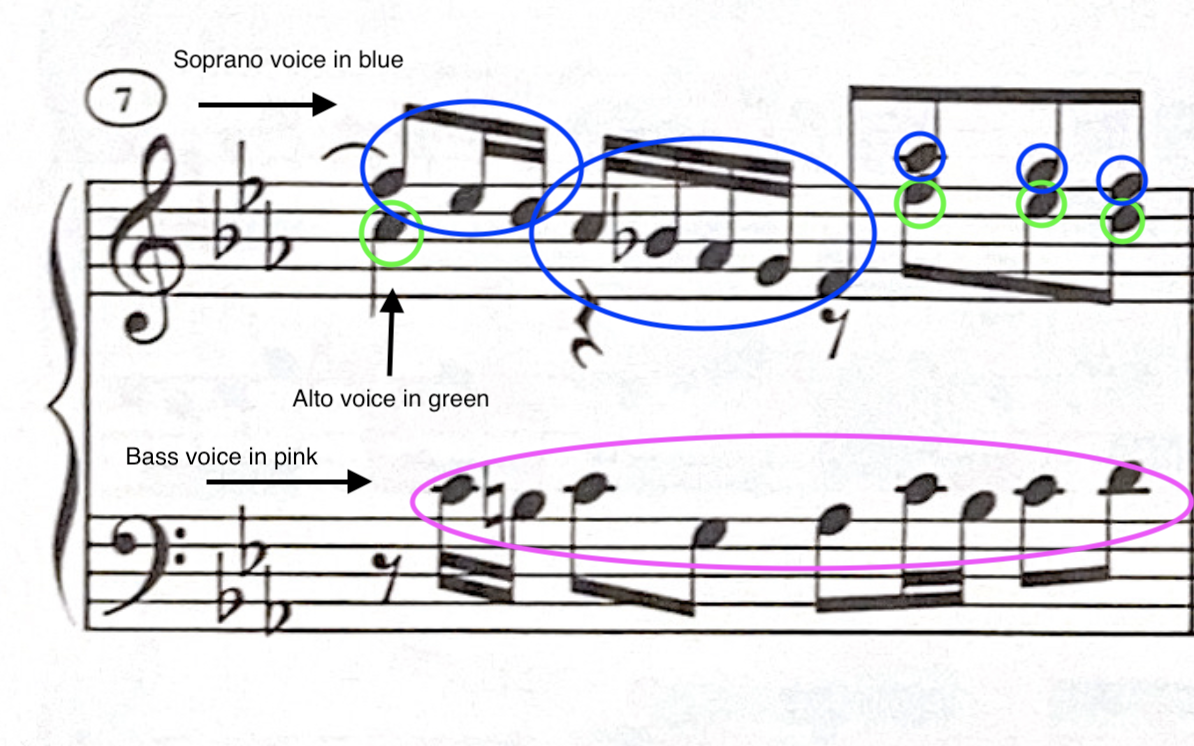
\includegraphics[width=.5\textwidth]{figures/fugue-three-voices.jpg}
    \caption{The three voices in Bach's \textit{Fugue in C Minor}}
    \label{fig:bach-fugue-three-voices}
\end{figure}
As seen in Figure \ref{fig:bach-fugue-three-voices}\autocite{Henle_2009}, there is a clear distinction between each voice. In the treble clef in the right hand, the top line whose stems face upwards make up the soprano line (the line and notes circled in blue), and the bottom line with stems faced downwards make up the alto line (the line and notes circled in green). The bass clef will only contain the bass voice (the bottom line, circled in pink), as this fugue is only in three voices. It is a balanced piece, with structure and interactions between the three voices, soprano, alto, and bass--or subject, and two countersubjects. Structurally, the fugue starts with an exposition which marks the introduction of the subject line in the alto voice, as in Figure \ref{fig:bach-fugue-subject}\autocite{Henle_2009}. This subject is then seen in the soprano and bass voices, as in Figures \ref{fig:bach-fugue-subject}\autocite{Henle_2009} and circled in pink in Figure \ref{fig:bach-fugue-three-voices}\autocite{Henle_2009}. The soprano voice is circled in blue, and the bass voice in pink, showcasing the subject in both voices.
\begin{figure}
    \centering
    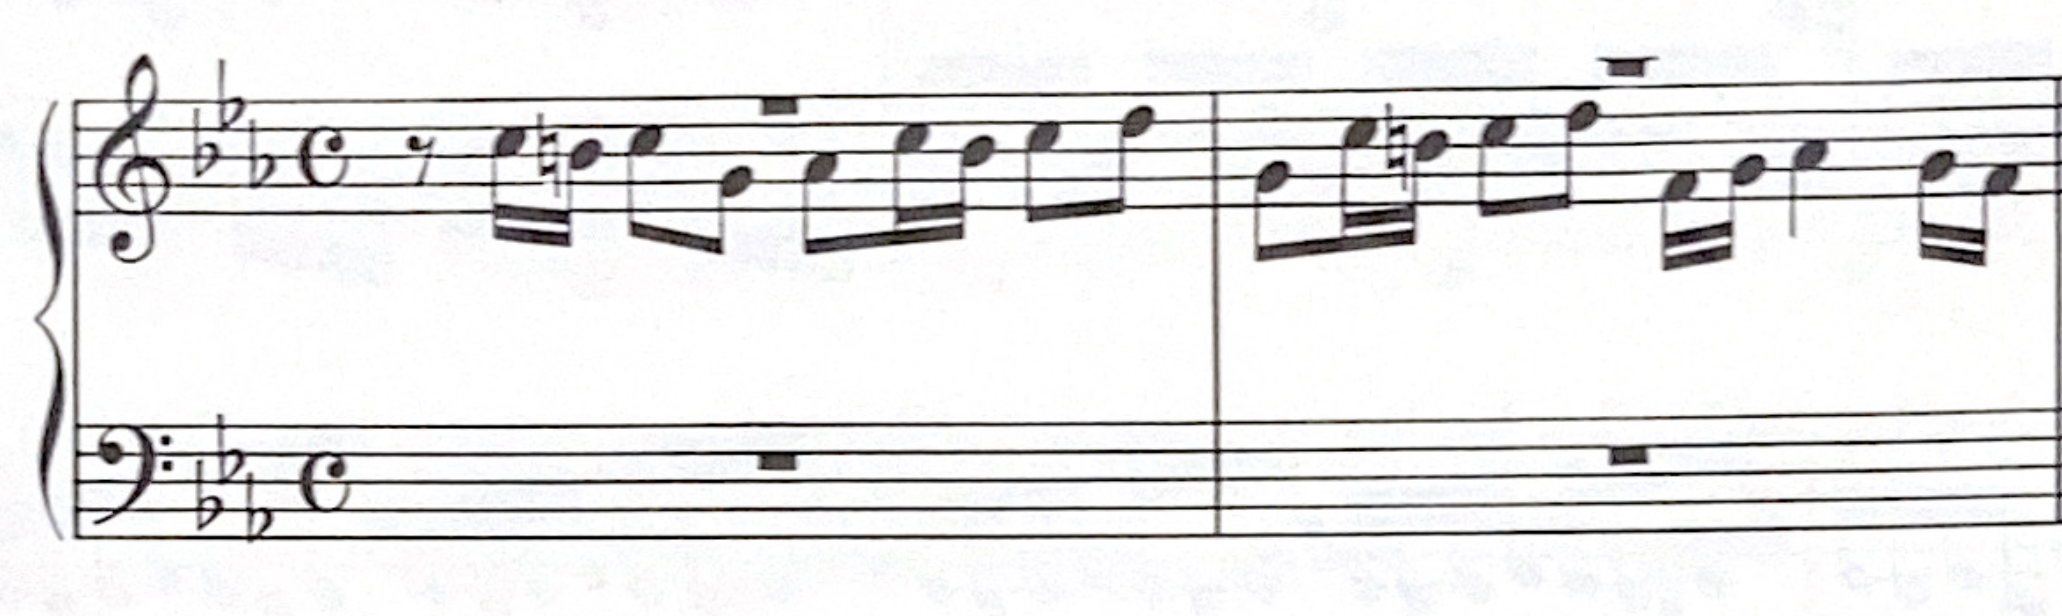
\includegraphics[width=\textwidth]{figures/bach-fugue-subject.jpg}
    \caption{The subject, in Bach's \textit{Fugue in C Minor}}
    \label{fig:bach-fugue-subject}
\end{figure}

The piece's third measure introduces the first countersubject in the alto voice, as in Figure \ref{fig:bach-fugue-first-countersubject}\autocite{Henle_2009}. Then, the second countersubject can be seen indicated rhythmically indicated in the second half of the first countersubject, before it is introduced on its own, as seen in Figure \ref{fig:bach-fugue-second-cs-indication}\autocite{Henle_2009}. The whole second countersubject then fully appears in the third and fourth beats of measure seven, circled in green, in Figure \ref{fig:bach-fugue-second-countersubject}\autocite{Henle_2009}.

\begin{figure}
    \centering
    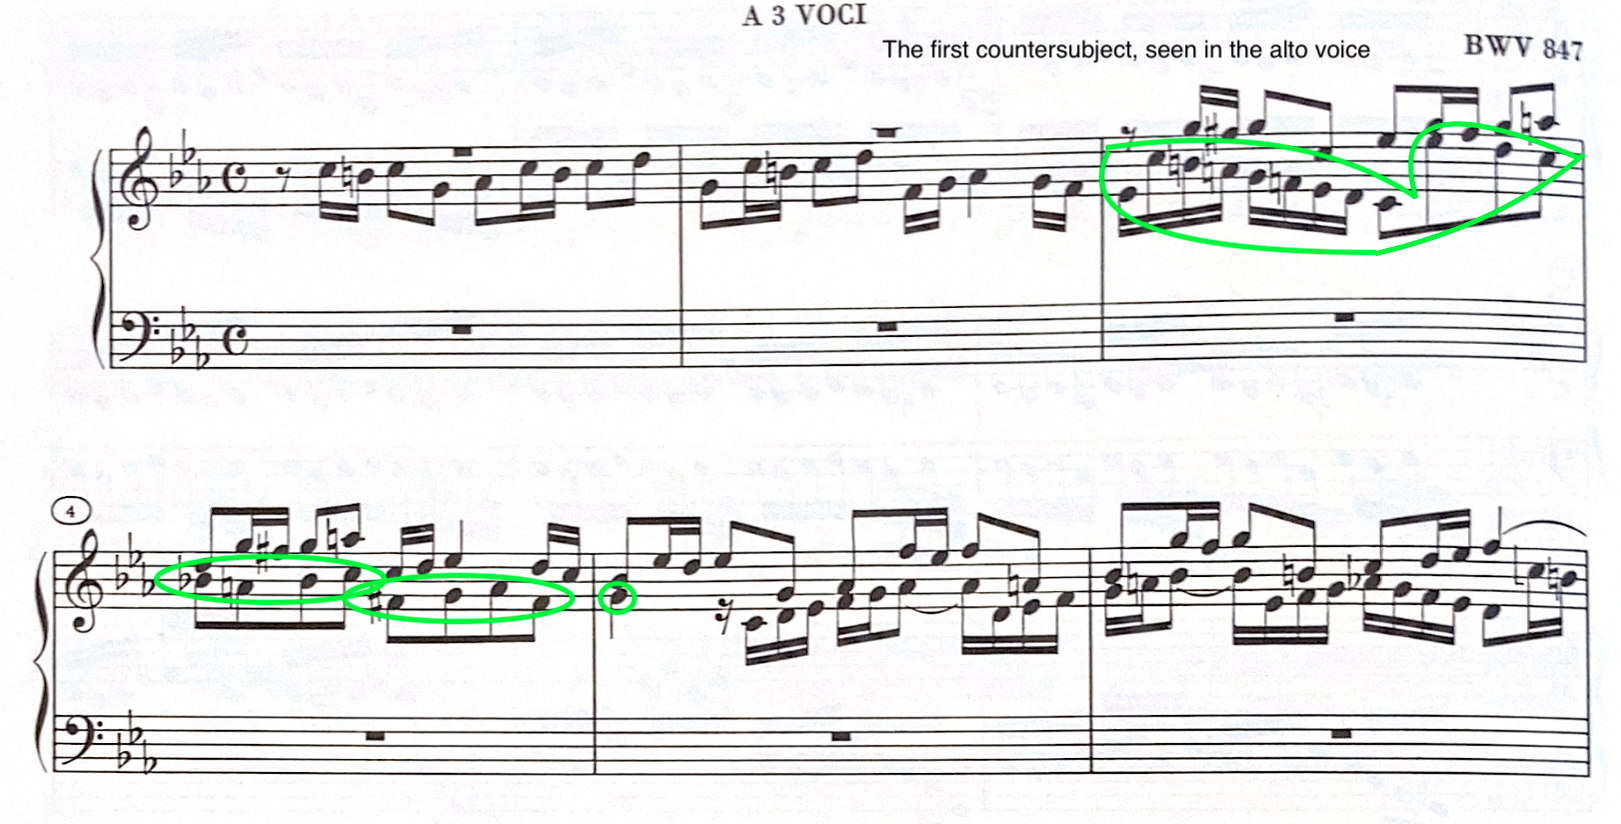
\includegraphics[width=\textwidth]{figures/bach-fugue-first-countersubject.jpg}
    \caption{The first countersubject, seen in the alto voice, in Bach's \textit{Fugue in C Minor}}
    \label{fig:bach-fugue-first-countersubject}
\end{figure}

\begin{figure}
    \centering
    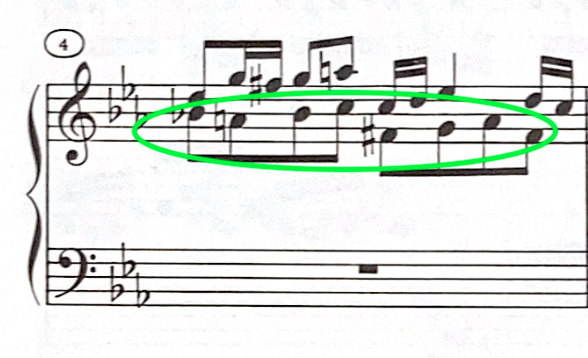
\includegraphics[width=0.5\textwidth]{figures/bach-fugue-second-cs-indication.jpg}
    \caption{The rhythmic indication of the second countersubject in Bach's \textit{Fugue in C Minor}, as circled in green, in the alto voice}
    \label{fig:bach-fugue-second-cs-indication}
\end{figure}

\begin{figure}
    \centering
    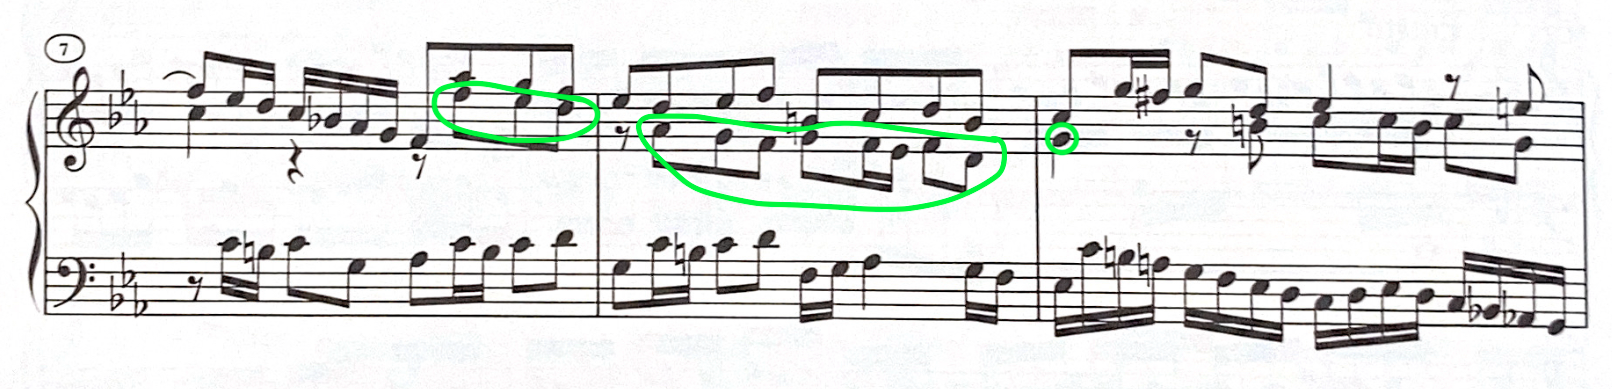
\includegraphics[width=\textwidth]{figures/bach-fugue-second-countersubject.jpg}
    \caption{The second countersubject, as found in the alto voice in its first appearance circled in green, from Bach's \textit{Fugue in C Minor}}
    \label{fig:bach-fugue-second-countersubject}
\end{figure}

Harmonically, the \textit{Fugue in C Minor} has a strong emphasis on minor keys, for dramatic effect. This is first seen in bar three of the \textit{Fugue in C Minor} in the top line, in Figure \ref{fig:bach-fugue-first-countersubject}\autocite{Henle_2009}, where the soprano voice modulates to the relative minor key, G harmonic minor. In the fugue's tension map\footnote{This is defined as a chart which details when there is tension in the music, and when the tension is resolved. Tension can be created through a chord's function, rhythm, or other methods.} there is more than a simple exposition\footnote{This is generally defined to be the section at the beginning of the piece, or near the beginning, in which one or more themes are presented according to a particular plan. These themes will be the basis of the rest of the movement or piece. In fugues specifically, the exposition is the opening section in which the voices enter one by one. Each voice states the principle theme (the subject), followed by the countersubject. All the voices after the fugue will wait to enter until the preceding voice has completed its statement of the subject.}\autocite{Walker_2001_Exposition}, subject entries, and coda\footnote{This is defined as the last part of a piece or melody, in which there is an implication that there is some addition being made to a standard form. In a fugue, this then refers to anything occurring after the last complete entry of the subject has been heard.}\autocite{Bullivant_2001}. 
\chapter[Mozart and Piano Sonata No. 10, K. 330]{Wolfgang Amadeus Mozart - Piano Sonata No. 10 in C major, K. 330 (1784)}\label{mozart}
Wolfgang Amadeus (W.A.) Mozart (1756-1791) was a prolific composer during the Classical period (1730-1820) of music. Mozart was born in Salzburg, in the Holy Roman Empire, on January 27, 1756\autocite{Burkholder_Grout_Palisca_2014}. He was born into a talented musical family, and by age five showed a prodigal ability in performance, specifically on the keyboard and violin \autocite{Eisen_Sadie_2001}. Mozart started performing as a court musician in the Salzburg court when he was 17, and began traveling. These travels eventually brought him to Vienna in 1781, where he chose to stay. While in Vienna, Mozart composed his \textit{Piano Sonata No. 10 in C Major}. This sonata has three movements, the allegro moderato in C Major, the Andante cantabile in F Major\footnote{This movement is in C Major's subdominant key, an important concept explained later.}, and the allegretto movement. 

The \textit{Piano Sonata in C Major} follows the standard structure of a sonata. A sonata is known to be an instrumental piece which contains one or more movements, and designed to be performed by either a soloist or a small ensemble\autocite{Mangsen_Irving_Rink_Griffiths_2014}. Each period of music had its own specific definition of a sonata, and the Classical period was no different\footnote{As stated by Mangsen et al., the definition of a sonata evolved. The definition of a sonata started generally as an instrumental piece in the thirteenth century, and was known as a \say{sonnade.} Through the development of instrumental music in the following centuries, the current definition of a sonata comes from its connotations and associations in the Classical and Romantic periods of music. The sonatas of these times were frequently assumed to be instrumental pieces in which one or more movements are incorporated. More information can be found in \citeauthor{Mangsen_Irving_Rink_Griffiths_2014} \citeyear{Mangsen_Irving_Rink_Griffiths_2014}}. Though definitions vary, generally the Classical period sonata is understood to be a musical work composed of three or four movements, most often for a piano solo \footnote{A duo between instruments such as the violin and piano were other popular choices.}. The first movement may be preceded by a slow introduction, but it is normally in sonata form. This is followed by a slow second movement, in which the key modulates to another, related key. Finally, the third movement follows as a finale, which wraps up the work.\autocite{Mangsen_Irving_Rink_Griffiths_2014} Sonata form itself is composed of three sections in a two-part tonal structure.\footnote{This two-part tonal structure is known as \say{binary form.} According to \citeauthor{Sutcliffe_Tilmouth_2001}, binary form is defined as a musical structure which consists of two sections, of roughly equal duration. This is often notated as \textit{AB}, or \textit{A$A^`$}. The form itself is characterized by the clear move to another key, followed by another clear return to the tonic key. At the end of the \textit{A} section, there is a conclusive-sounding arrival on a contrasting key (which is often the dominant key) to signify the end of the \textit{A} section. The \textit{B} section's key will then modulate to the key that was referenced at the end of the \textit{A} section. At the end of the \textit{B} section, there is a matching conclusive arrival to what we saw at the end of the \textit{A} section, this time returning to the tonic key found in the \textit{A} section. Both the \textit{A} and \textit{B} sections may also be marked by a repeat sign, to be played through twice. More information can be read in \citeauthor{Sutcliffe_Tilmouth_2001} \citeyear{Sutcliffe_Tilmouth_2001}} 

Of the three movements of the sonata form, we divide them into two tonal parts. First, there is the \say{exposition} section, which is the first in the two-part tonal structure. The exposition, as the first section in both the sonata form and the two-part tonal structure, will contain the themes through which the rest of the movement and the piece are to be based on. The exposition will open in the piece's tonic key, and concludes in a new key. This new key is typically the dominant key of the exposition section's key if the piece is in a major key\autocite{Webster_2001}--which is a fifth interval away from the key in the exposition. With the exposition conclusively arriving in a new key, the piece moves to the \say{development} section. Once the development section arrives, we have moved into the second part of the two-part tonal structure. This part of the tonal structure includes both the development and recapitulation\autocite{Webster_2001}. The development section takes the thematic material that was presented in the exposition section, and manipulates it, moving both themes and key away from the exposition.\footnote{Some of these thematic manipulations include reshaping the material on a motivic level, on a harmonic level, or on a counterpoint level, or some combination of these levels.} The ending of the development section will lead into the \say{recapitulation} section. This recapitulation section is the final section of the sonata form, and is also a part of the second section of the two-part tonal structure. It signifies the return to the tonic key of the exposition section\autocite{Webster_2001}, and restates the thematic material from that first section.

\section{Movement I: Allegro moderato}
The first movement in Mozart's \textit{Piano Sonata in C Major} is the Allegro moderato. As is typical of sonatas, this first movement is light and energetic, evidenced by Mozart's choice to use cut-time (two-four time instead of the more widely used four-four time), and the thirty-second notes instead of sixteenth-notes, like in figure \ref{fig:mozart-thirty-second-notes}\autocite{Henle_1977}. There are two main themes, or subjects, which alternate between legato and staccato. These subjects are placed over an energetic bass voice, comprised of flowing eighth and sixteenth notes.

\begin{figure}
    \centering
    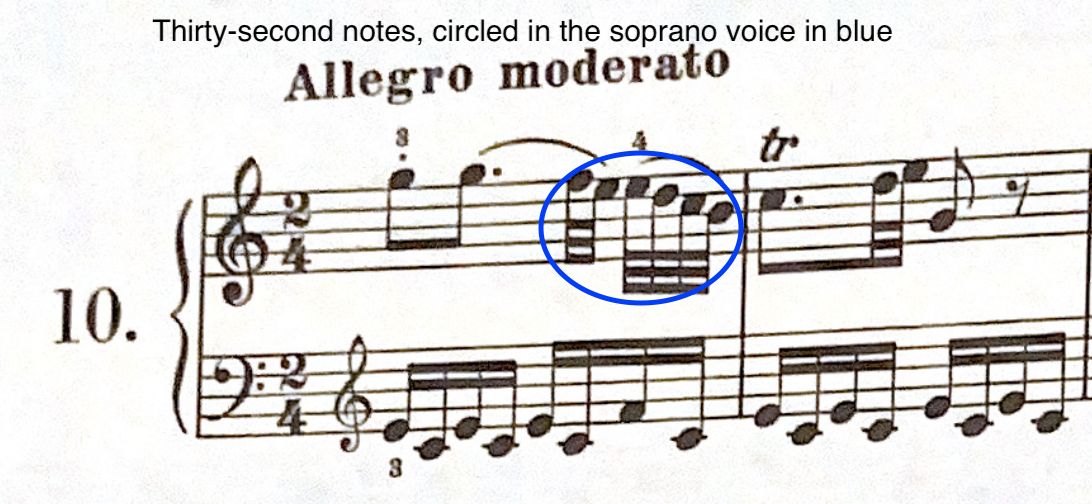
\includegraphics[width=0.5\textwidth]{figures/mozart-thirty-second-notes.png}
    \caption{An example of thirty-second notes, seen in Mozart's \textit{Piano Sonata in C Major}}
    \label{fig:mozart-thirty-second-notes}
\end{figure}

\begin{figure}
    \centering
    \includegraphics[width=\textwidth]{figures/mozart-first-movement-first-theme.png}
    \caption{The first of two themes seen in Mozart's \textit{Piano Sonata in C Major}}
    \label{fig:mozart-first-movement-first-theme}
\end{figure}

\begin{figure}
    \centering
    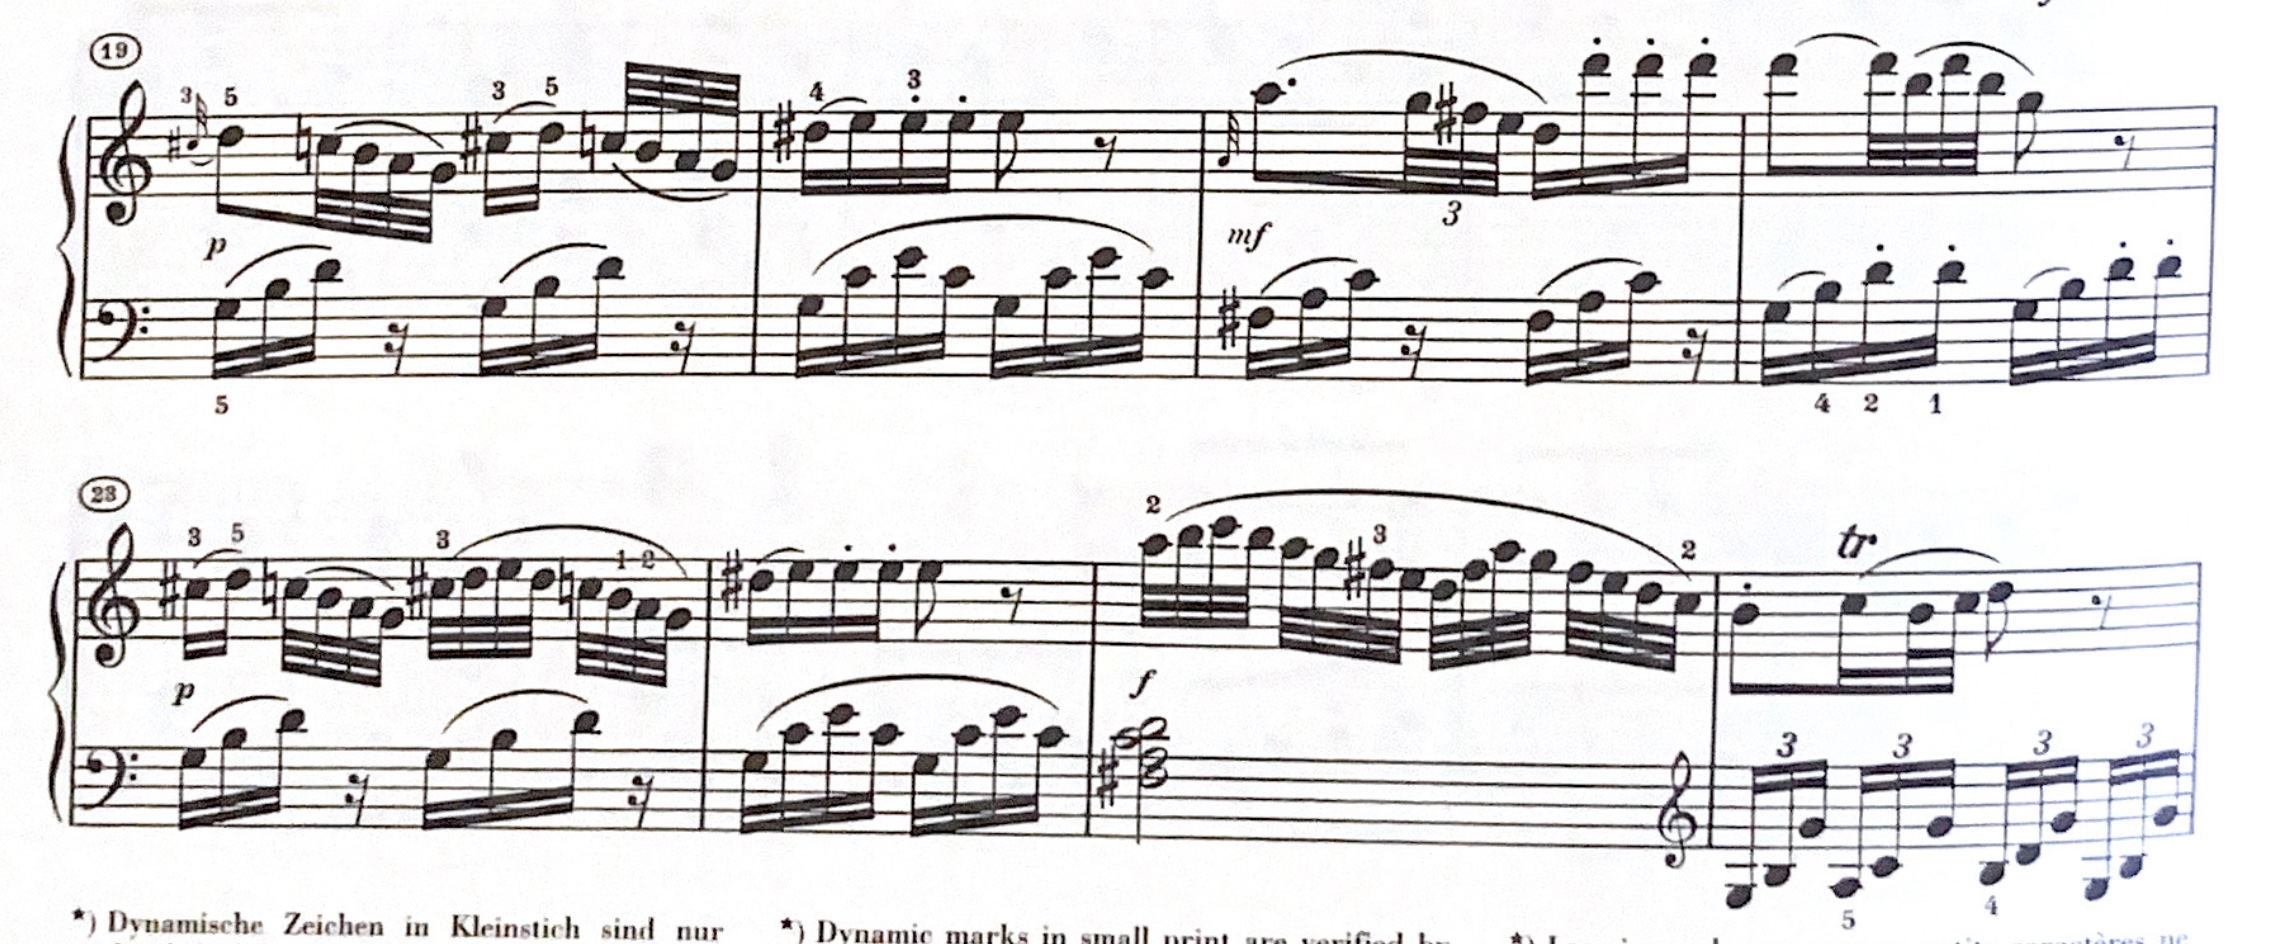
\includegraphics[width=\textwidth]{figures/mozart-first-movement-second-theme.jpg}
    \caption[The second theme in Mozart's \textit{Piano Sonata in C Major, K. 330}]{The beginning of the second of the two themes seen in Mozart's \textit{Piano Sonata in C Major}}
    \label{fig:mozart-first-movement-second-theme}
\end{figure}

The movement has two major themes, each decorated with ornamentation\footnote{This is defined as the decoration of a melodic or harmonic line in music. More reading can be found in \citeauthor{Latham_2011} \autocite{Burkholder_Grout_Palisca_2014}}. The first twelve bars of the movement begin the exposition section. Within this section, we have two themes. The first theme, as seen in figure \ref{fig:mozart-first-movement-first-theme}\autocite{Henle_1977}, lasts from bars one through twelve, and marked in red. This theme starts in the piece's tonic key of C Major. The second theme in figure \ref{fig:mozart-first-movement-second-theme}\autocite{Henle_1977} begins in bar nineteen, and is marked by a modulation to G Major, the dominant key of the piece's tonic key C Major. The exposition section sets up the primary theme of the movement as a whole. The first theme, which is seen in figure \ref{fig:mozart-first-movement-first-theme}\autocite{Henle_1977}, will be the theme through which the remainder of the movement is based on. The exposition's second theme, from figure \ref{fig:mozart-first-movement-second-theme}\autocite{Henle_1977}, is also elaborated upon later in the piece. 

There is a development section introduced in bar fifty-nine, as in figure \ref{fig:mozart-first-movement-development-start}\autocite{Henle_1977}. This section is more intense than the exposition section, with more modulations. Bar sixty-nine and bar seventy show the modulation to A Major\footnote{See figure \ref{fig:mozart-first-movement-modulation-a-major} \citeauthor{Henle_1977}}. This section also modulates to F Major\footnote{See figure \ref{fig:mozart-first-movement-f-major} \citeauthor{Henle_1977}}, D Minor\footnote{See figure \ref{fig:mozart-first-movement-d-minor} \citeauthor{Henle_1977}}, before modulating back to the tonic key of C Major for the recapitulation section. In addition to the many modulations to related keys to the tonic C Major, the development section also contains references to thematic material of the first section. The bass voice in the first theme of the exposition section, as in figure \ref{fig:mozart-first-movement-first-theme}\autocite{Henle_1977}, contains energetic sixteenth notes for the entirety of the theme. This is referred to in the development section, with bars fifty-nine to sixty-three, as in figure \ref{fig:mozart-first-movement-development-reference-first-theme}\autocite{Henle_1977}, bracketed in red. 

\begin{figure}
    \centering
    \includegraphics[width=\textwidth]{figures/mozart-first-movement-development-reference-first-theme.png}
    \caption{The reference to the first theme in the exposition section, found in the development section, in Mozart's \textit{Piano Sonata in C Major}}
    \label{fig:mozart-first-movement-development-reference-first-theme}
\end{figure}

\begin{figure}
    \centering
    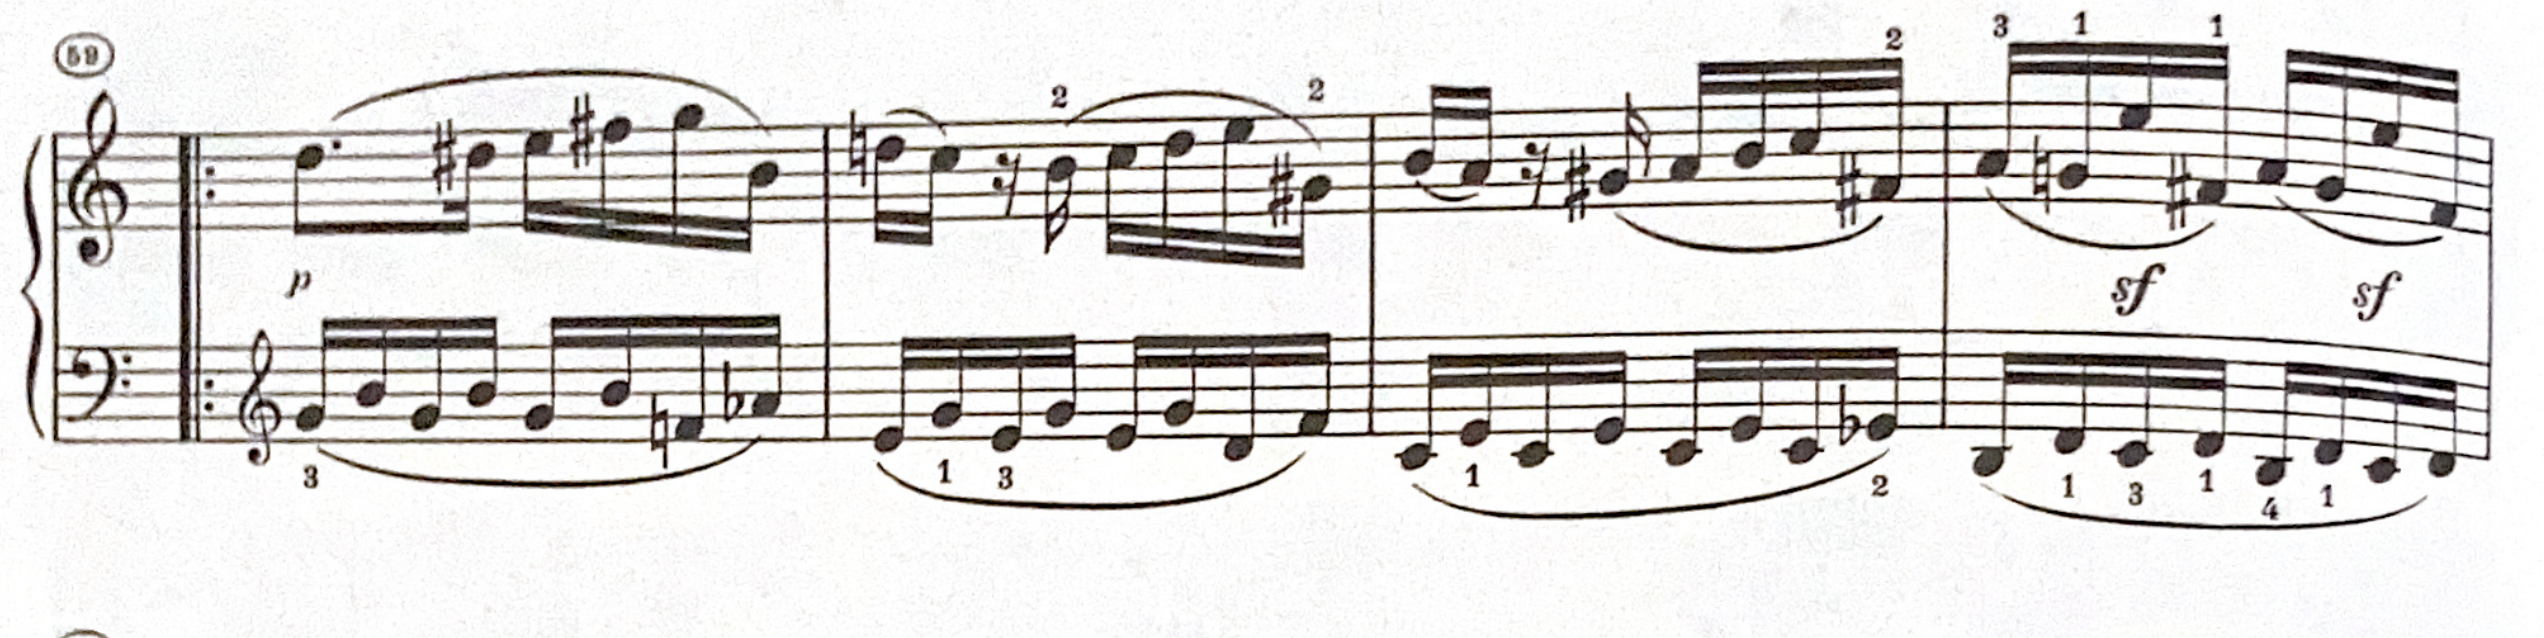
\includegraphics[width=\textwidth]{figures/mozart-first-movement-development-start.png}
    \caption{The beginning of the development section in the first movement of Mozart's \textit{Piano Sonata in C Major}}\autocite{Henle_1977}
    \label{fig:mozart-first-movement-development-start}
\end{figure}

\begin{figure}
    \centering
    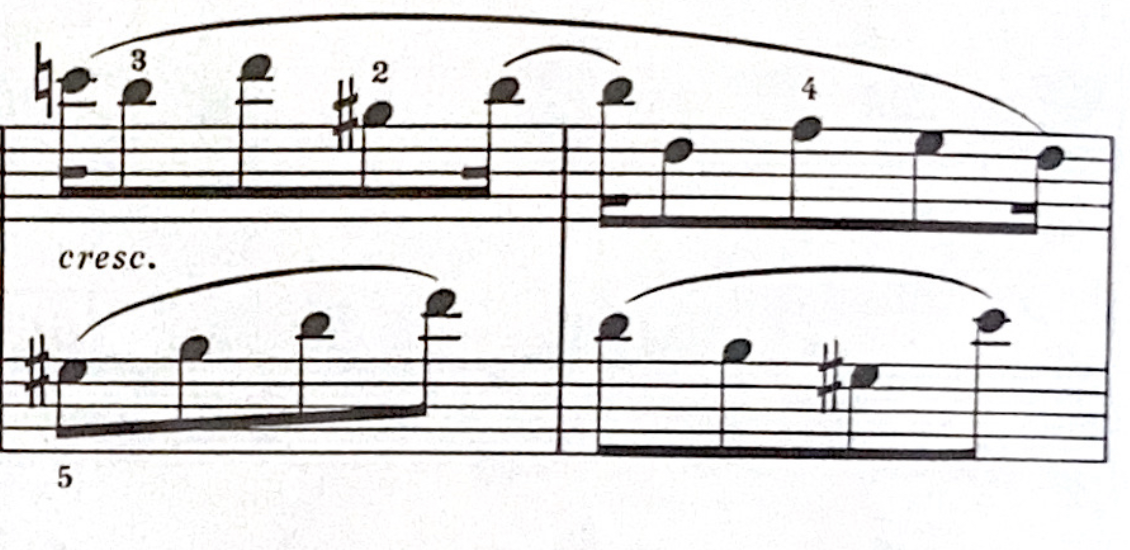
\includegraphics[width=0.5\textwidth]{figures/mozart-first-movement-modulation-a-major.png}
    \caption{The modulation to A Major, in Mozart's \textit{Piano Sonata in C Major}}
    \label{fig:mozart-first-movement-modulation-a-major}
\end{figure}

\begin{figure}
    \centering
    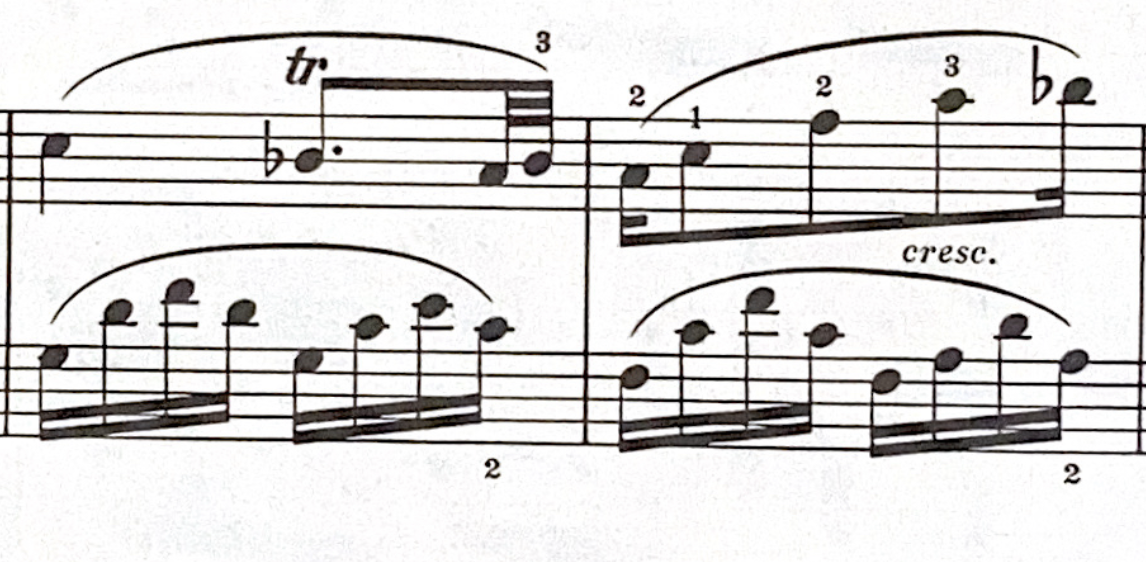
\includegraphics[width=0.5\textwidth]{figures/mozart-first-movement-f-major.png}
    \caption{The modulation to F Major, in Mozart's \textit{Piano Sonata in C Major}}
    \label{fig:mozart-first-movement-f-major}
\end{figure}

\begin{figure}
    \centering
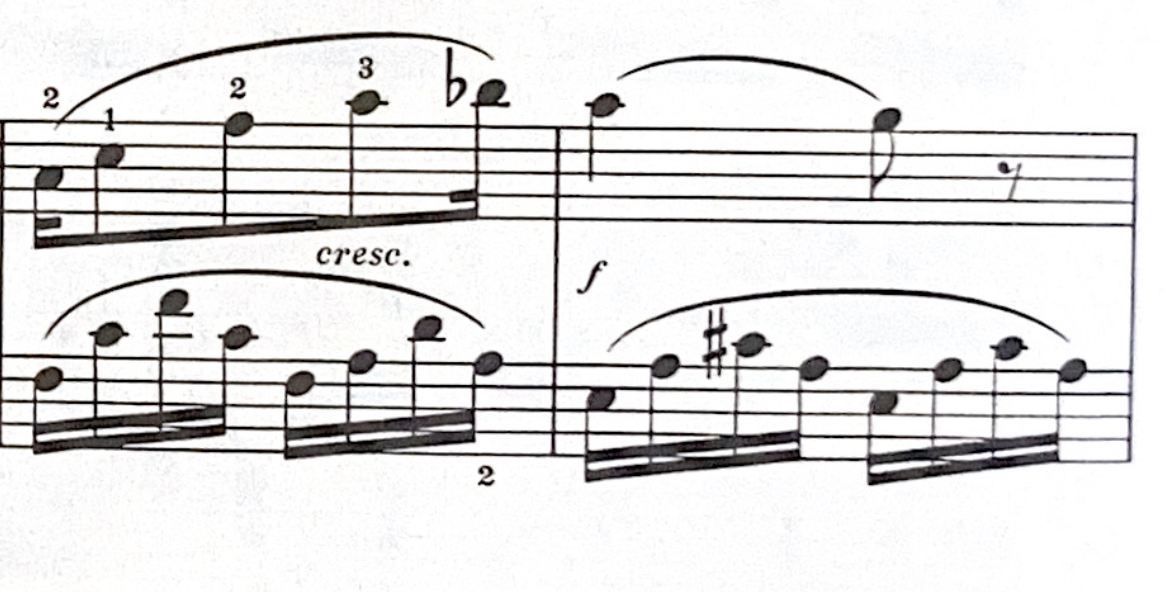
\includegraphics[width=0.5\textwidth]{figures/mozart-first-movement-d-minor.png}
    \caption{The modulation to D Minor, in Mozart's \textit{Piano Sonata in C Major}}
    \label{fig:mozart-first-movement-d-minor}
\end{figure}

\begin{figure}
    \centering
    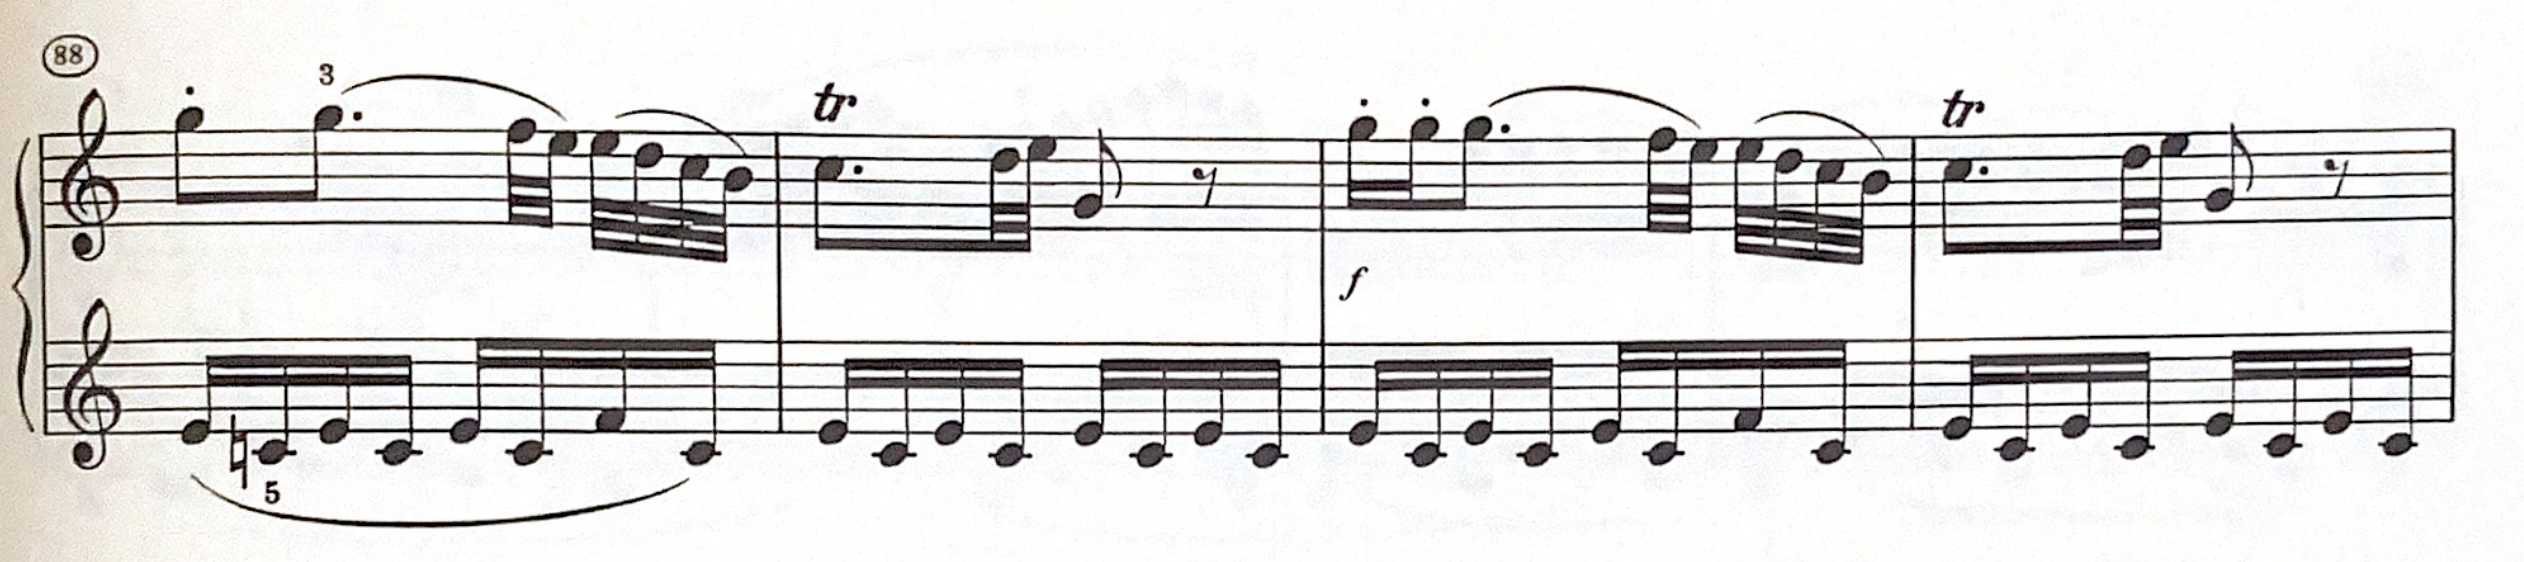
\includegraphics[width=\textwidth]{figures/mozart-first-movement-recapitulation-first-theme.png}
    \caption[The first theme of the exposition, found in the recapitulation, from Mozart's \textit{Piano Sonata in C Major, K. 330}]{The recapitulation section in Mozart's \textit{Piano Sonata in C Major}, where the first theme from the exposition section is heard again}
    \label{fig:mozart-first-movement-recapitulation-first-theme}
\end{figure}

Finally, in the recapitulation section, the first subject is heard again, in C Major, as in figure \ref{fig:mozart-first-movement-recapitulation-first-theme}\autocite{Henle_1977}. The recapitulation section is similar in structure to the exposition section, with the first theme in tonic key C Major, and the second theme in dominant key G Major. There are few changes made to these two themes in this section, beyond a higher amount of ornamentation added to various bars. Thus, we see that the first movement itself is also in sonata form, with an exposition section, development section, and recapitulation section.

\section{Movement II: Andante cantabile}

The second movement of Mozart's \textit{Piano Sonata in C Major}, the Andante cantabile, is marked with the modifier \say{cantabile,} meaning \say{song-like} and is reflected in the overall tonality of this movement being similar to a very sweet song. This movement is in ternary form\footnote{Ternary form is a musical structure which consists of three sections, hence the qualifier ternary. Its representation may be in the form of letter scheme ABA, with the final section A being a repetition of the first section. Each section of the ternary form is usually, but not always, self-contained and closes (or ends) in its key. The first A section will normally close in the tonic key. Then, the middle section will provide a strong contrast to the two sections which surround it, both in tone and theme.} and in the key F Major. This is important to note, as this is a modulation from the first movement, in which the key was C Major. This movement has the tonic key in F Major, whose dominant key is now C Major. The beginning 'A' section, as seen in figure \ref{fig:mozart-second-movement-first-a-section}\autocite{Henle_1977} and bracket in red, is a twenty-bar melody, broken into two sections by the repeat, and contains a repeated-note motif. The first section is comprised of the first eight bars, from the beginning up to the repeat sign\footnote{See figure \ref{fig:mozart-second-movement-first-a-section} \citeauthor{Henle_1977}}. This repeated-note motif is seen in the opening's frequent use of the note 'C' in figure \ref{fig:mozart-second-movement-first-eight-bars}\autocite{Henle_1977}\footnote{The first eight bars are bracketed in red.}. There are four repeated C's, of which the note C is imitated and repeated several times through these eight bars.

\begin{figure}
    \centering
    \includegraphics[width=\textwidth]{figures/mozart-second-movement-first-a-section.png}
    \caption{The first A section of the second movement of Mozart's \textit{Piano Sonata in C Major}}
    \label{fig:mozart-second-movement-first-a-section}
\end{figure}

\begin{figure}
    \centering
    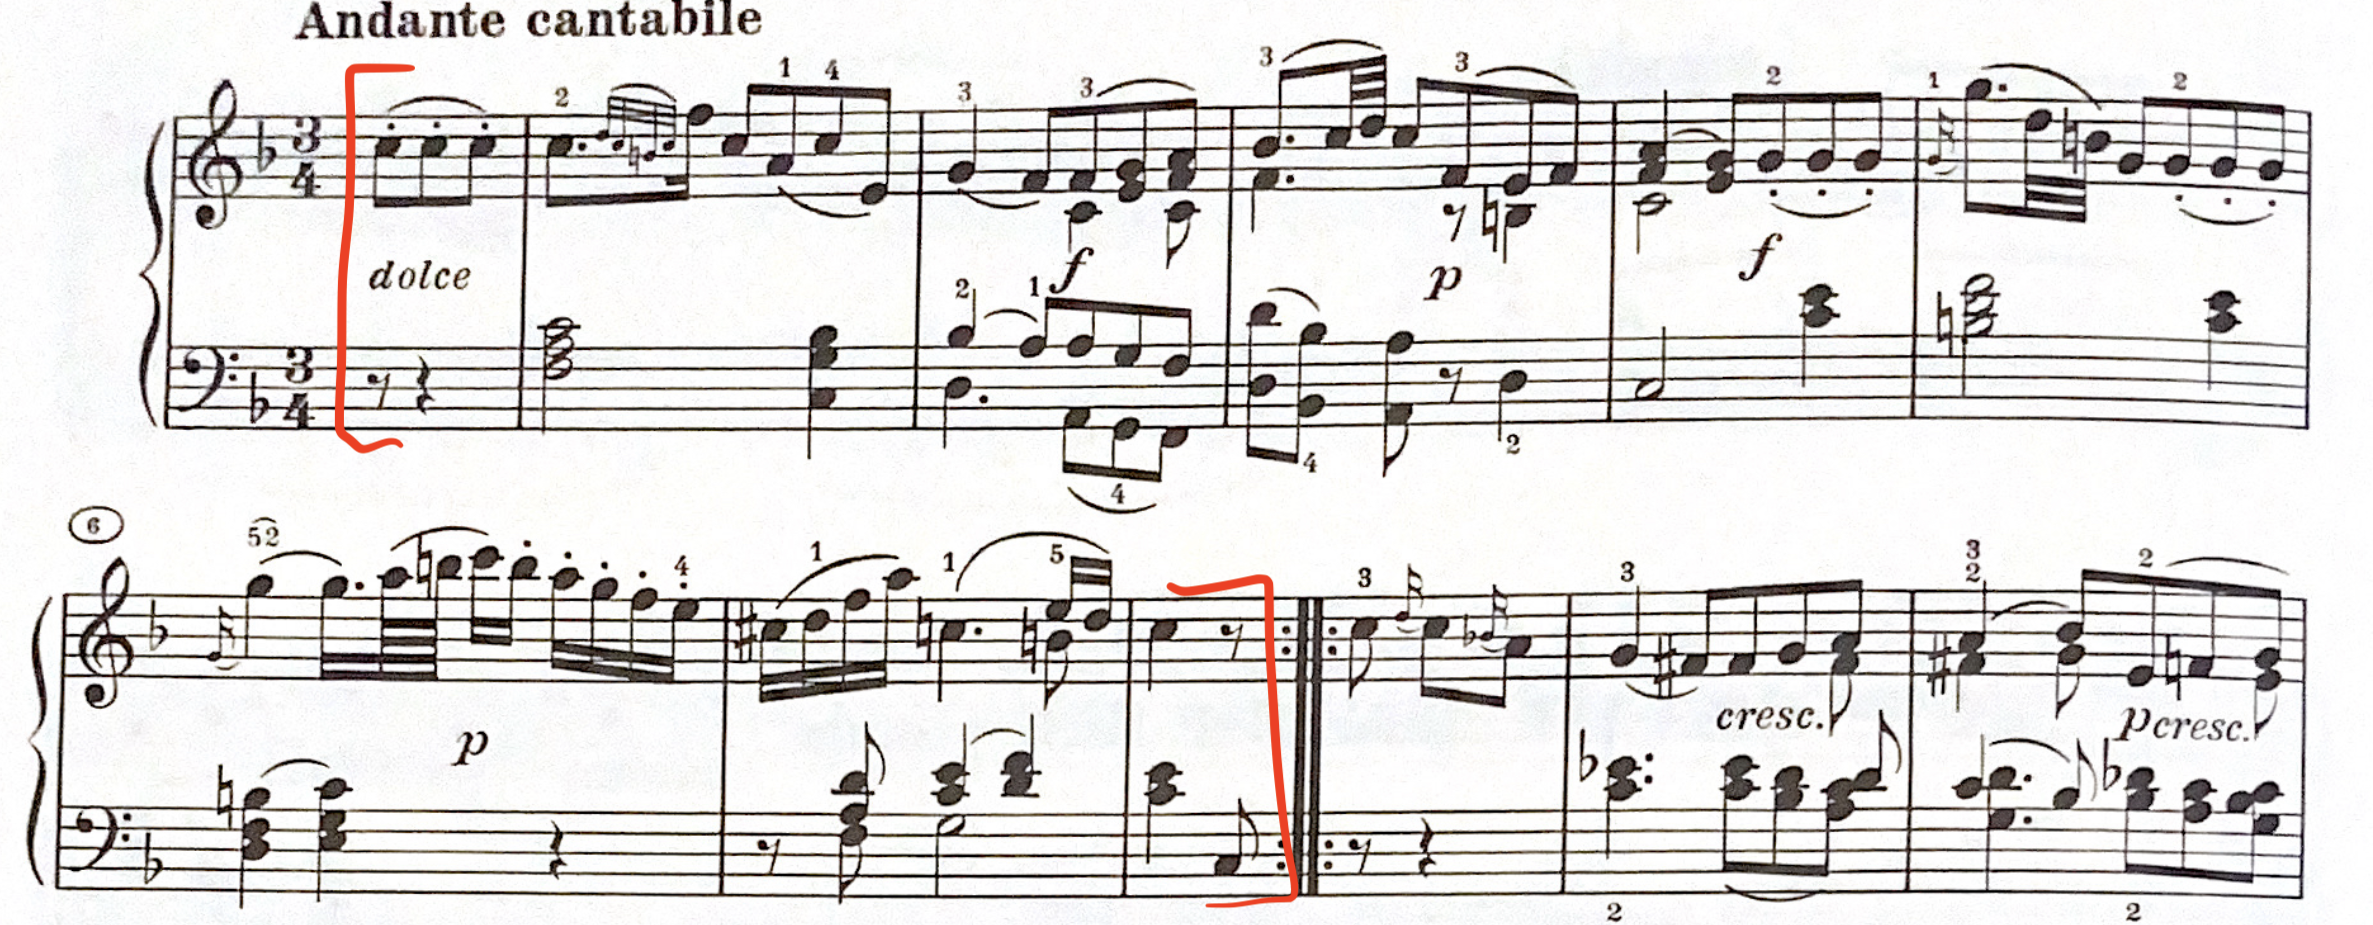
\includegraphics[width=0.5\textwidth]{figures/mozart-second-movement-first-eight-bars.png}
    \caption{The first eight bars of the second movement of Mozart's \textit{Piano Sonata in C Major}}
    \label{fig:mozart-second-movement-first-eight-bars}
\end{figure}

\begin{figure}
    \centering
    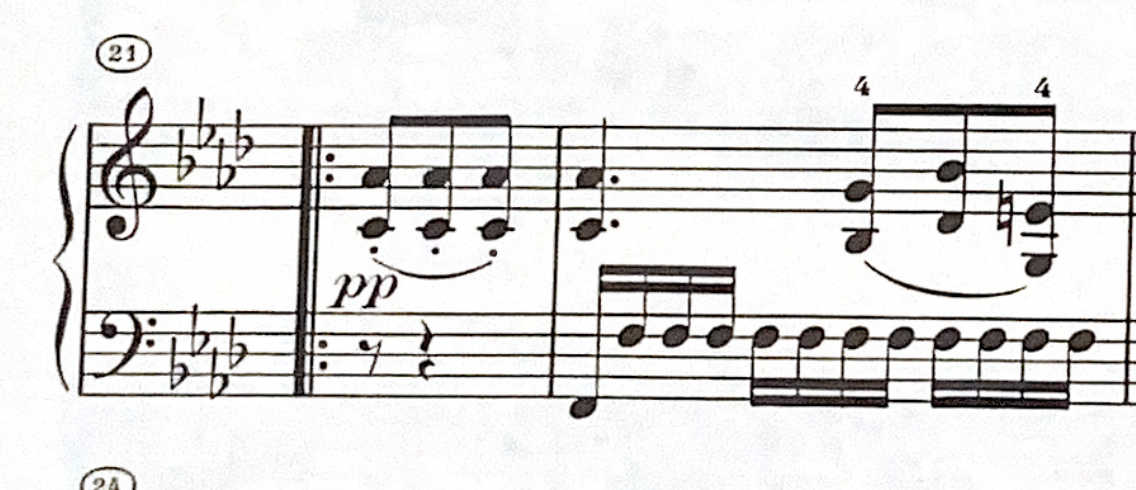
\includegraphics[width=0.5\textwidth]{figures/mozart-second-movement-repeated-note-motif-middle-section.png}
    \caption{The repeated-note motif, found in the middle section of Mozart's \textit{Piano Sonata in C Major} of the second movement}
    \label{fig:mozart-second-movement-middle-section-motif}
\end{figure}

After the repetition, the middle section turns to the movement's tonic minor key\footnote{So, going from the movement's tonic key of F Major to its minor key of F Minor.}. Its melody starts in bar twenty-one, reminiscent and similar to the preceding section, with similar rhythm and usage of a repeated-note motif, as in figure \ref{fig:mozart-second-movement-middle-section-motif}\autocite{Henle_1977}. From here, it is clear to see that the first movement in of itself contains the format of a sonata form: there is an exposition, development, and recapitulation section.

\section{Movement II: Allegretto}
The third movement of Mozart's \textit{Piano Sonata in C Major}, the Allegretto, is the piece's most energetic movement. The use of arpeggios, or the sounding of a chord's notes in succession rather than in unison\autocite{Arpeggio_2001}\footnote{Arpeggios are noticeable in keyboard music, in which a chord is much more easily able to be spread out or broken apart. The keyboard is much more built for an arpeggio figuration, as each note of a chord can be played independently much easier on it.}, is prevalent throughout the movement. This movement also shares several characteristics with the first movement, including the most important: the sonata form. The third movement itself has the form of a sonata, as did the first movement, with an exposition, development, and recapitulation section. The exposition section contains a similar-sounding dotted-eighth note motif as in the first movement, as seen in figure \ref{fig:mozart-third-movement-dotted-eighth-notes-and-exposition}\autocite{Henle_1977}. The development section, on the other hand, has no relation with the material worked on within the exposition section. Its thematic material instead consists of its own figures, solely found in this section. Finally, the recapitulation features a short coda, as seen in figure \ref{fig:mozart-third-movement-coda}\autocite{Henle_1977}, and full chords. This ends the movement and the piece on a triumphant-sound, as is typical of the sonata form.

\begin{figure}
    \centering
    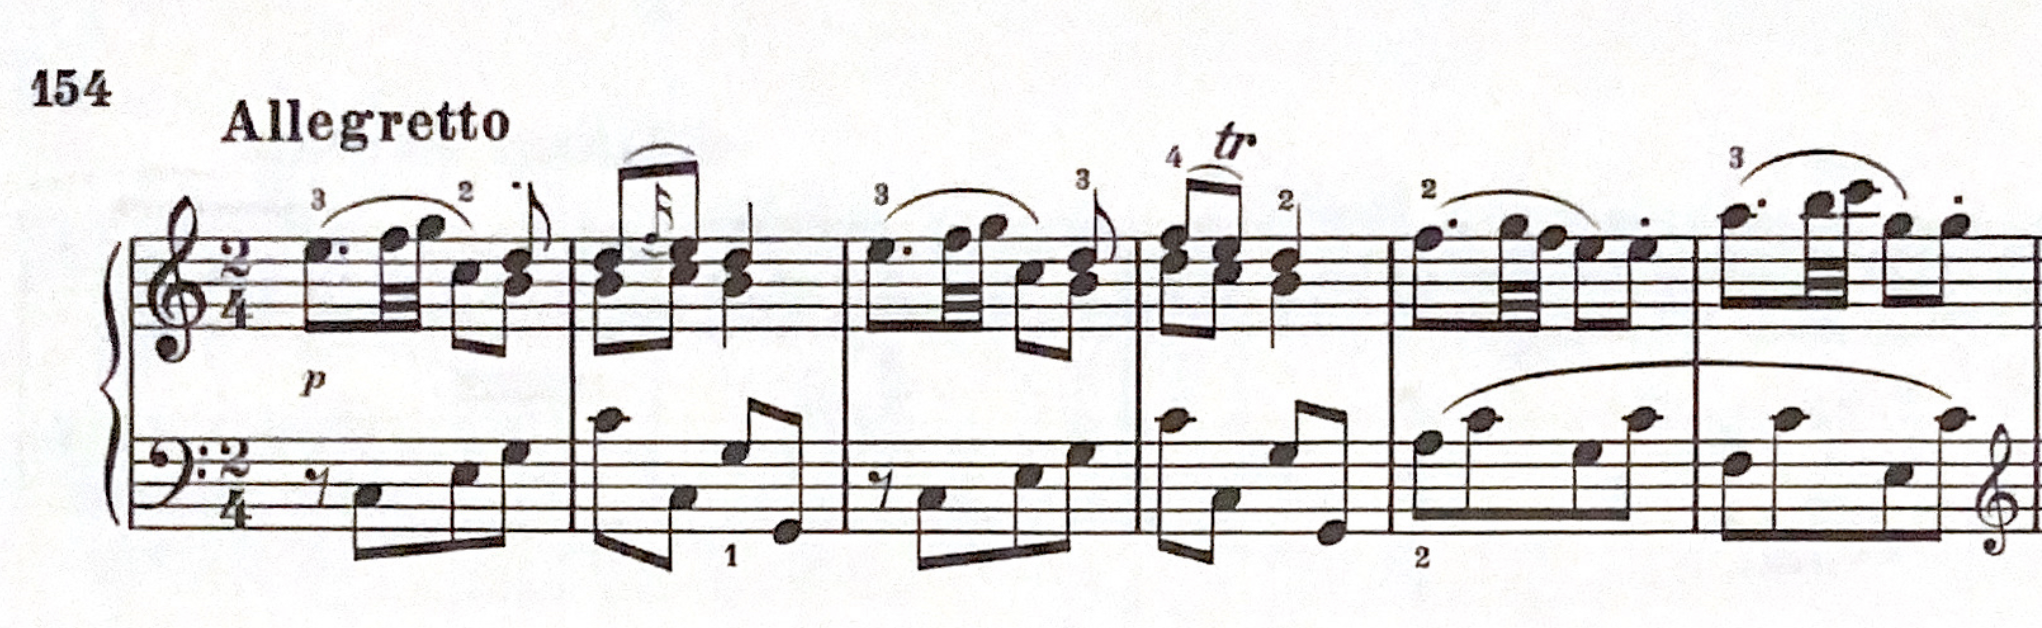
\includegraphics[width=\textwidth]{figures/mozart-third-movement-dotted-eighth-notes-and-exposition.png}
    \caption{The dotted-eighth note motif in the third movement of Mozart's \textit{Piano Sonata in C Major}}
    \label{fig:mozart-third-movement-dotted-eighth-notes-and-exposition}
\end{figure}

\begin{figure}
    \centering
    \includegraphics[width=\textwidth]{figures/mozart-third-movement-coda.png}
    \caption{Mozart's \textit{Piano Sonata in C Major}, the coda of the third movement}
    \label{fig:mozart-third-movement-coda}
\end{figure}

\chapter[Beethoven and Eleven Bagatelles, Op. 119, No. 1]{Ludwig van Beethoven - \textit{Eleven Bagatelles,} Op. 119, No. 1 (1803)}\label{chapter:beethoven}

Ludwig van Beethoven (1770-1827) was a composer who rose to prominence towards the end of the Classical period. He was born in Bonn, in Northwest Germany, where both his father and grandfather were court musicians in Cologne. His works have been divided into three periods: his birth until approximately 1802, from 1803-1814, and finally from 1815 to his death in 1827 \autocite{Kerman_Tyson_Burnham_Johnson_Drabkin_2001}, reflecting stylistic changes and important life events. In the first period, Beethoven mastered the popular genres and musical concepts of his time and crafting his style. He studied with Joseph Haydn (another Classical era composer), and Johann Georg Albrechtsberger, learning the art of counterpoint. This led to compositions of wide-use, including virtuosic works and pieces for beginner piano students\autocite{Burkholder_Grout_Palisca_2014}, and private works for connoisseurs and public symphonies. Then in 1802, Beethoven experienced a gradual loss of hearing, which would render him fully deaf in a few years. With the support from patrons and sales to publishers, he was able to compose works of a new depth, reflected by the struggles he was facing in life. Finally, in the third period, his music became more introspective and difficult for performers to play and listeners to comprehend\autocite{Kerman_Tyson_Burnham_Johnson_Drabkin_2001}. By 1818, his hearing had worsened to near-deafness, and this prompted another change in style. This period featured a higher degree of contrast than before \autocite{Burkholder_Grout_Palisca_2014}, and exaggerated. There was contrast between style, figuration, meter, and tempo. To balance the contrasts, there was also an emphasis on continuity, blurring divisions between phrases or movements.

The bagatelle form is a short piece of music, sometimes defined to literally be \say{something short, a trifle}, and is composed to be light-hearted\autocite{Brown_2001}. The title \say{bagatelle} itself does not imply any specific musical form, and the term has been used as a generic title since Beethoven's three sets of bagatelles for piano (Opus 33, 119, and 126). His later two sets of bagatelles (Opus 119 and Opus 126) are anything but simple and a trifle. These two sets reflect the introspective second period of Beethoven, as his hearing declined. 

\section{Bagatelle, Op. 119, No. 1}
The first of the bagatelles in Beethoven's Opus 119, this bagatelle is in ternary form, a three-part musical form, typically notated as \textit{ABA`}. The final section, \textit{A`}, is a repeat of the first \textit{A} section. Each section of the form is self-contained, usually closing in its own key\autocite{Tucker_Cochrane_2011}. Thus, the A section will close in the tonic key, and the A` section will modulate to another, related key, and closes in that key.\footnote{This key will typically be the dominant or relative major key of the one in the first A section.} The middle section, the \textit{B} section of a ternary piece will provide a strong contrast to the two \textit{A} sections which surround it, contrasting both in theme and tonality.

The first section of the Bagatelle, the \textit{A} section, begins with a theme which sounds light and bouncy, but has a more subdued tonality. In the first four bars of this section, the articulation is hard to miss, as in Figure \ref{fig:beethoven-first-a-section-first-four-bars}. The first immediate element the performer will notice is the usage of articulation, specifically staccato. This gives the beginning of the movement a very bouncy character, juxtaposed with the otherwise mysterious nature of the A section. Beethoven also employs the use of phrase functions and phrase ends, which help a performer treat what the piece \say{says} in the style of the composer. Rests, as a form of articulation, are carefully placed throughout the A section. This causes the performer to ensure that they pause at appropriate times through the piece. 

In the first eight bars of the A section, as seen in Figure \ref{fig:beethoven-first-a-section-first-eight-bars}\autocite{Henle_1978} and demarcated in red brackets, can clearly be broken into several parts. The first four measures of the section, as in Figure \ref{fig:beethoven-first-a-section-structure}\autocite{Henle_1978}, are a repeat of each other. Bars three and four repeat bars one and two, but are only a minor third interval lower. The two parts which make up the A section are marked with the use of a quarter rest in between, in bar four. This second half of the section's first eight bars, what will be known as the \say{continuation,} is to give the listener the feeling that there is an ending coming \autocite{Kerman_Tyson_Burnham_Johnson_Drabkin_2001}. This ending is normally signified by the use of quicker rhythms and an increase in harmonies. Finally, in bar eight this sensed ending appears, but not in an expected way. Bar eight contains a half-cadence, a type of cadence\footnote{A cadence can be defined as a melodic or harmonic motion, which is typically associated with the ending of a phrase, section, movement, or composition.}\autocite{Nagley_Whittall_2011} which ends the phrase on a dominant chord, here being the chord D Major. So, the phrase ends with unresolved harmonic tension, and implies that another phrase will follow it.

\begin{figure}
  \centering
  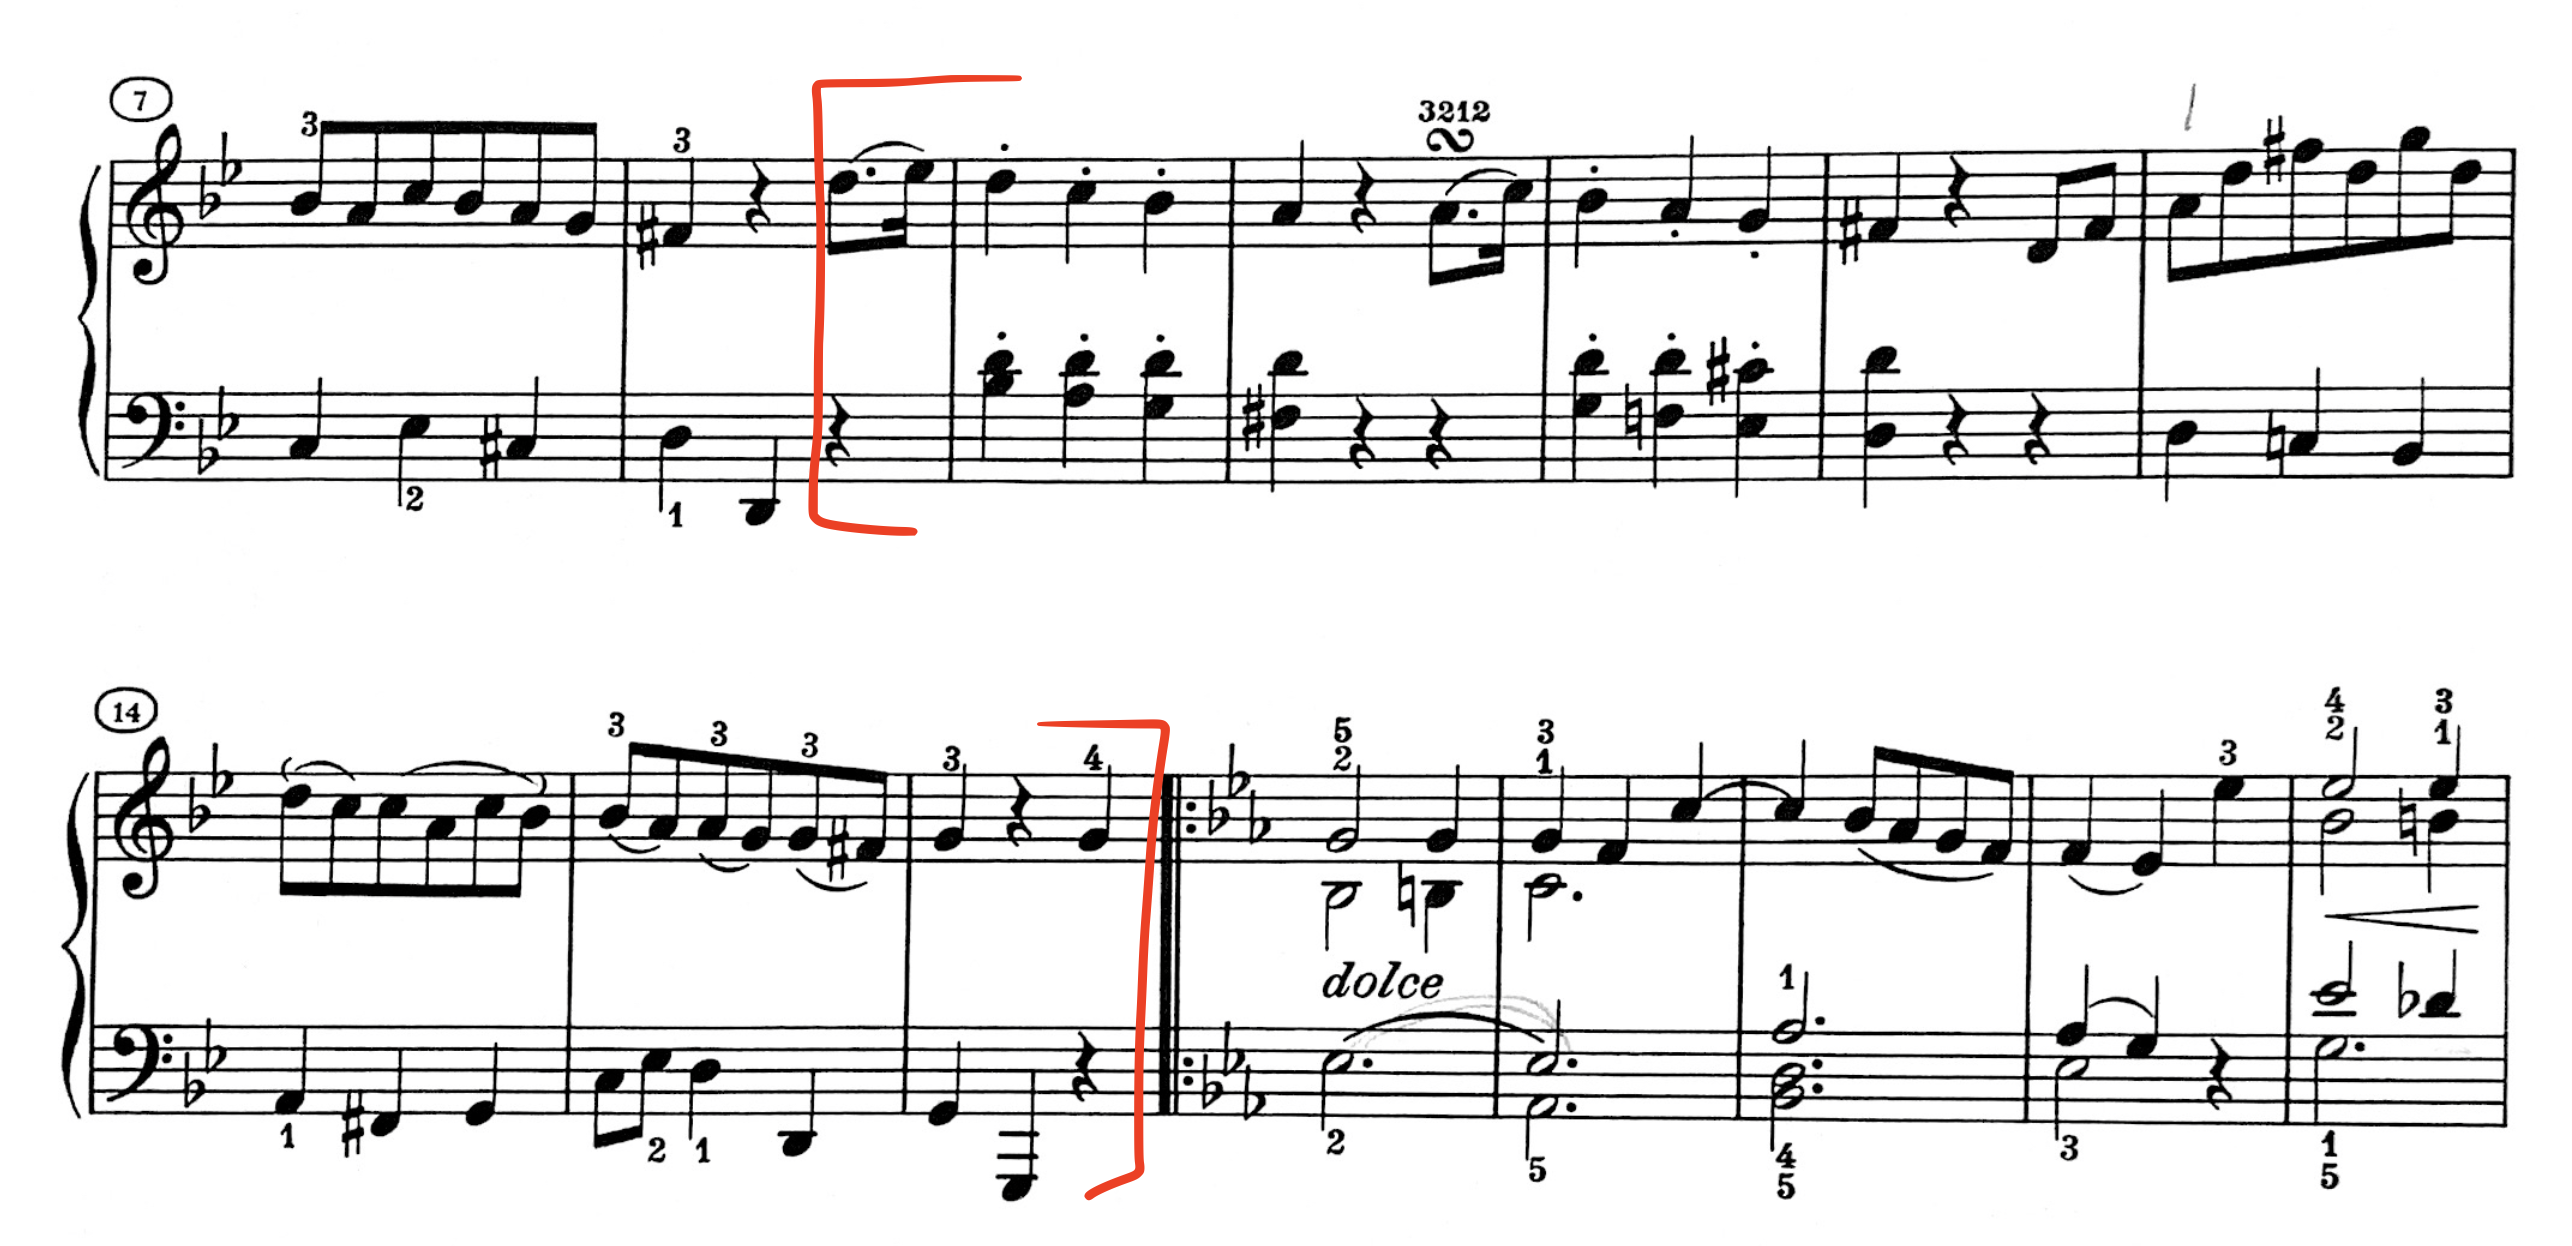
\includegraphics[width=\textwidth]{figures/beethoven-first-a-section-bars-nine-to-sixteen.jpg}
  \caption{Bars nine to sixteen of Beethoven's \textit{Eleven Bagatelles}, Opus 119}
  \label{fig:beethoven-first-a-section-bars-nine-to-sixteen}
\end{figure}

\begin{figure}
	\centering
	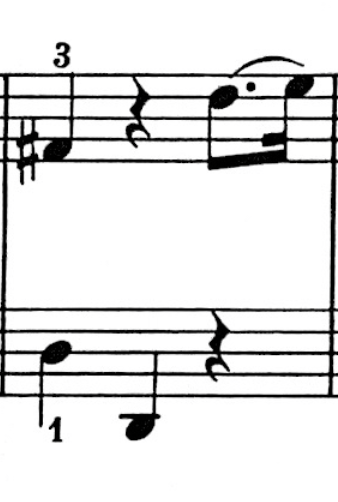
\includegraphics[width=0.4\textwidth]{figures/beethoven-first-a-section-hc.jpg}
	\caption{Half-cadence in Beethoven's \textit{Eleven Bagatelles}, Opus 119}
	\label{fig:beethoven-first-a-section-hc}
\end{figure}

\begin{figure}
	\centering
	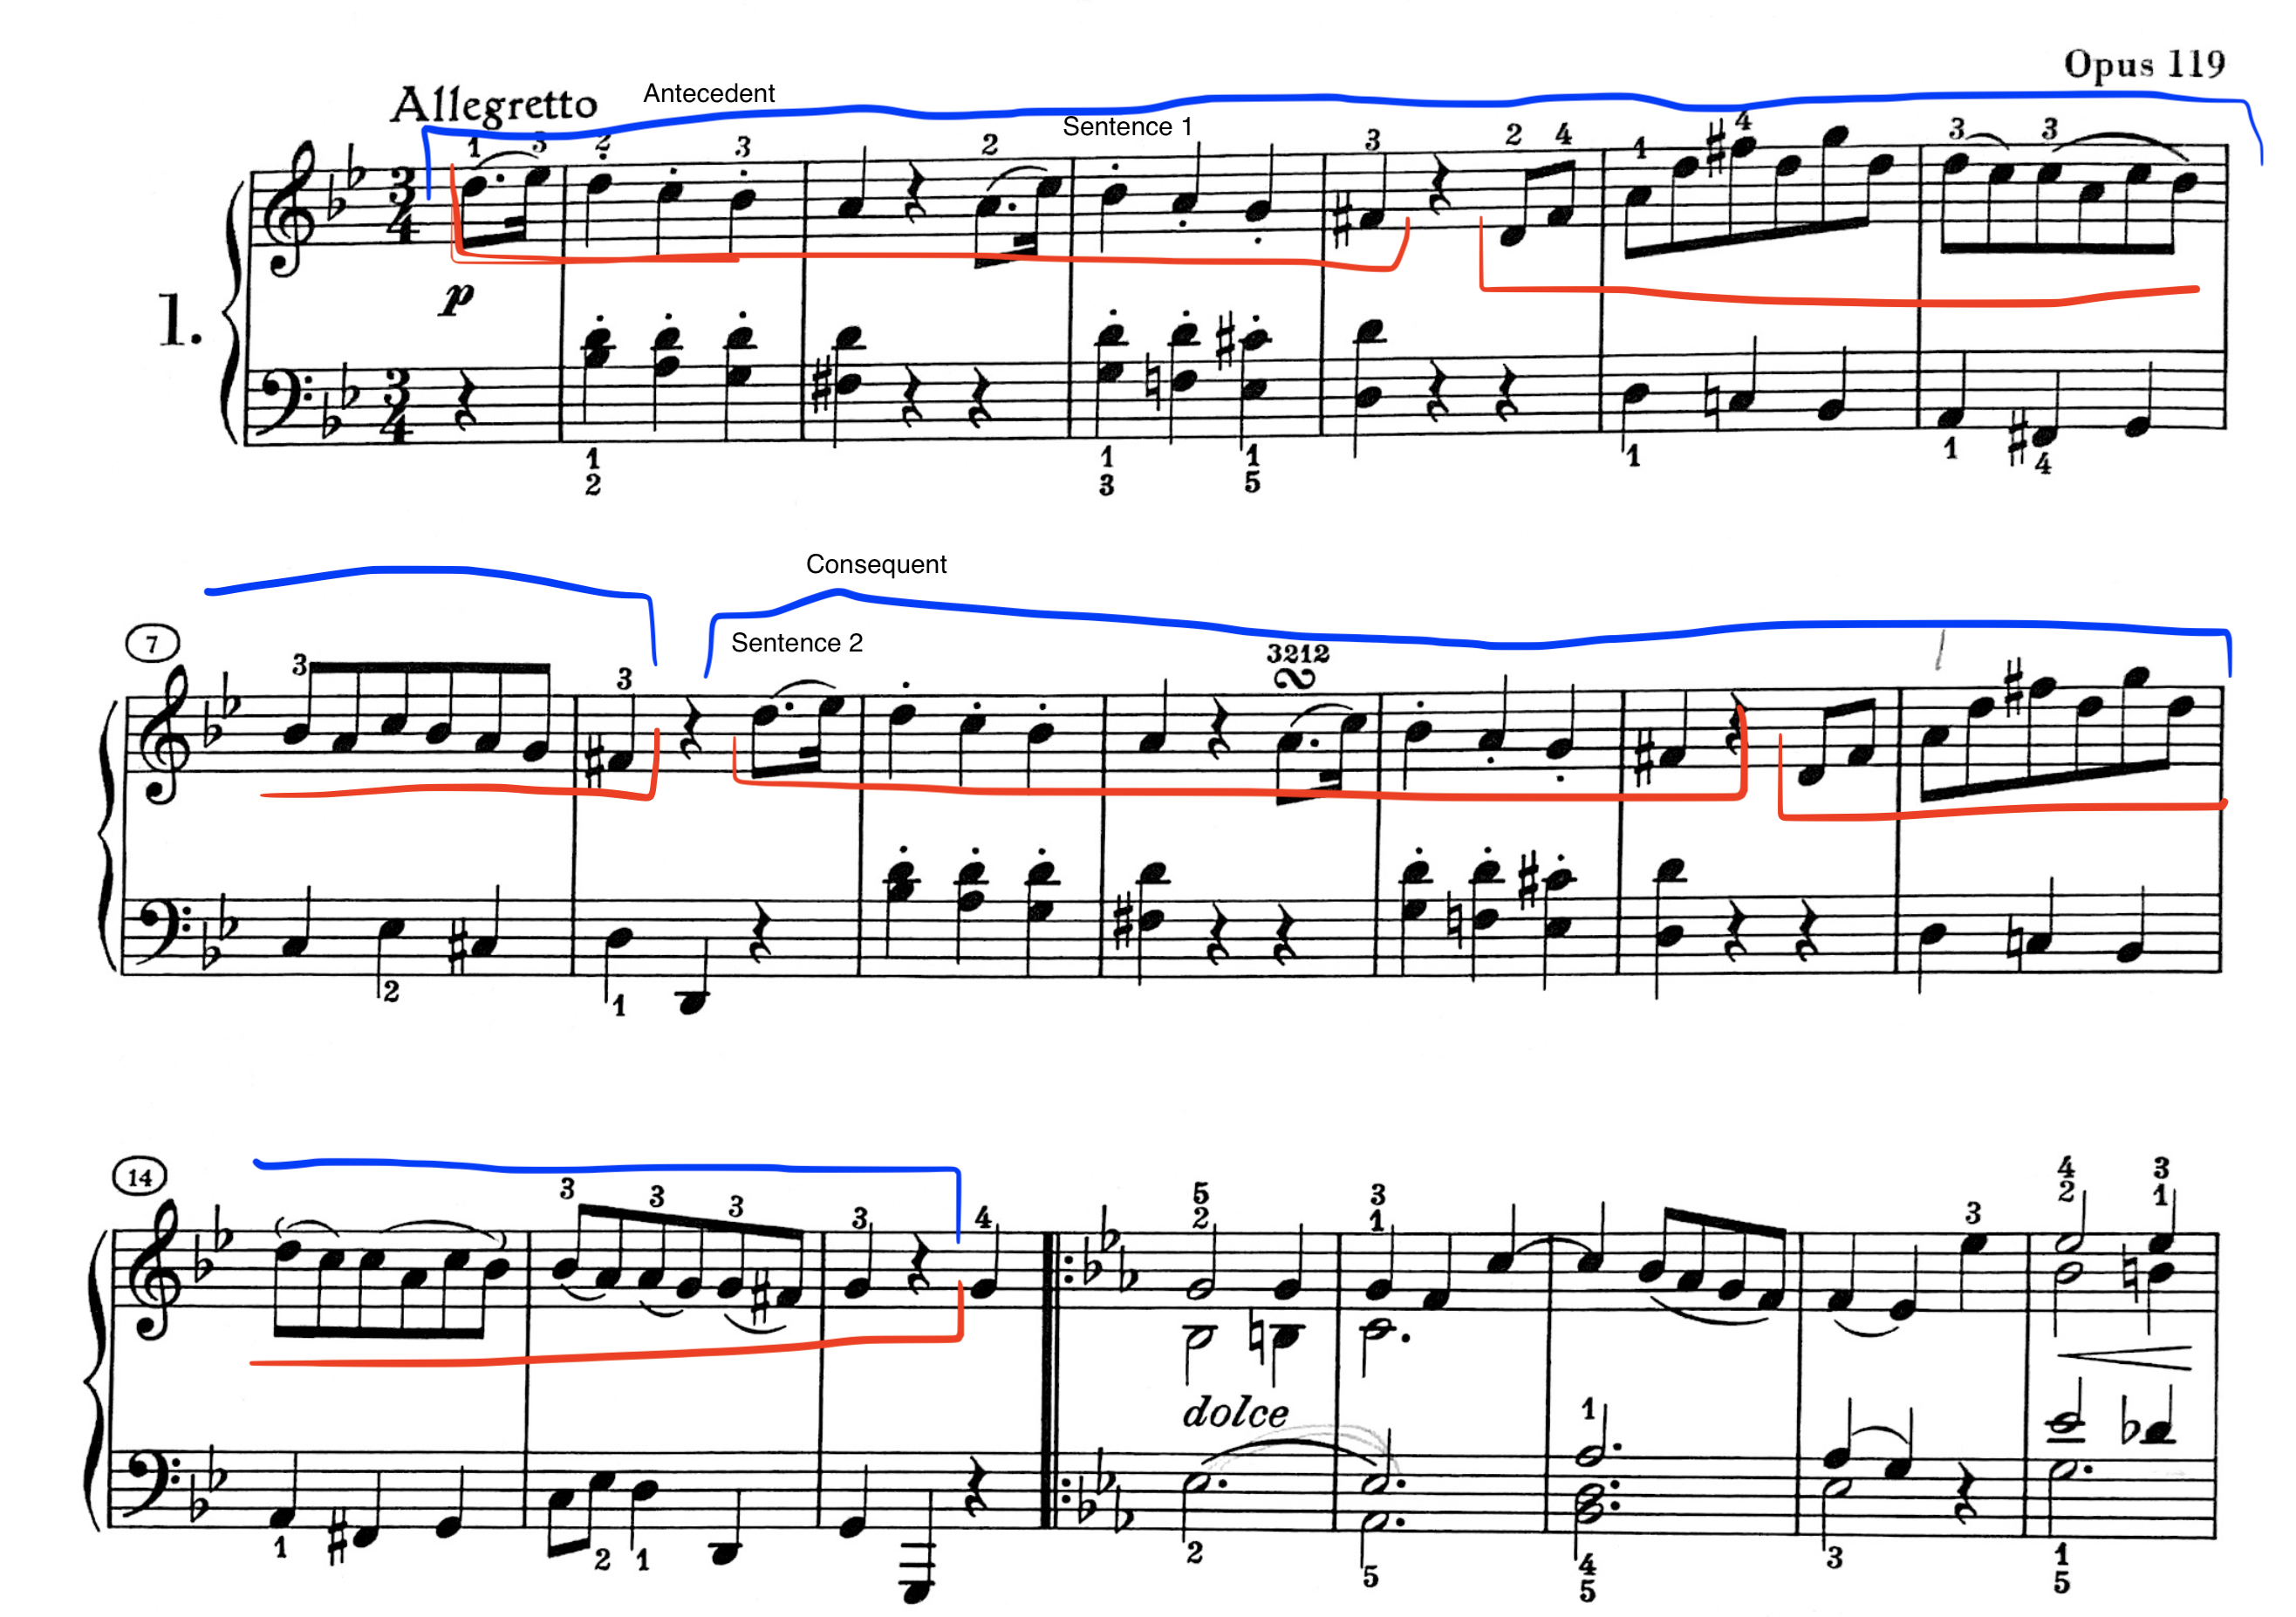
\includegraphics[width=0.5\textwidth]{figures/beethoven-first-a-section-structure.jpg}
	\caption{The structure of the first A section in Beethoven's \textit{Eleven Bagatelles}, Opus 119}
	\label{fig:beethoven-first-a-section-structure}
\end{figure}

Bar nine of the section, as in Figure \ref{fig:beethoven-first-a-section-bars-nine-to-sixteen}\autocite{Henle_1978} and bracketed in red, is an exact repeat of bar one. Thus, there is a larger organizational structure to this piece, and the first A section, than the first eight bars of the section.\footnote{These first eight bars of the A section form a sentence. A sentence in music is defined as a complete musical idea, such as a self-contained theme, which is the sum or two or four phrases arranged in a complementary manner.} As bars one through eight are almost repeated exactly in bars nine through sixteen, albeit not immediately, this signals the structure known as a period. A period is similar to a sentence; it has two parts: the antecedent and the consequent, which are bracketed in blue in Figure \ref{fig:beethoven-first-a-section-structure}\autocite{Henle_1978}. Each section starts exactly the same, but end differently. The antecedent phrase sets up the musical idea that will be treated during the period, and ends on a weak type of cadence, including the half-cadence, or deceptive cadence. The consequent phrase, which follows the antecedence, repeats the idea found in the antecedent phrase, and ends with a stronger cadence (such as the perfect authentic cadence, or PAC), signifying the end of a phrase. The repeat of material first found in bar one in bar nine signals to the performer that there is a period. There is a half-cadence in bar eight, as in Figure \ref{fig:beethoven-first-a-section-hc}\autocite{Henle_1978}, which is a weak cadence. Then, bars nine through sixteen contain material that is repeated. In bar sixteen, instead of a half-cadence ending the phrase, there is a PAC, ending the phrase in the tonic key. As seen in Figure \ref{fig:beethoven-first-a-section-structure}\autocite{Henle_1978}, the period which makes up the first A section is a nested period, in that in the period itself, there are two sentences nested inside. The section will come back in the end of the piece, in the \textit{A`} section. 

\begin{figure}
	\centering
	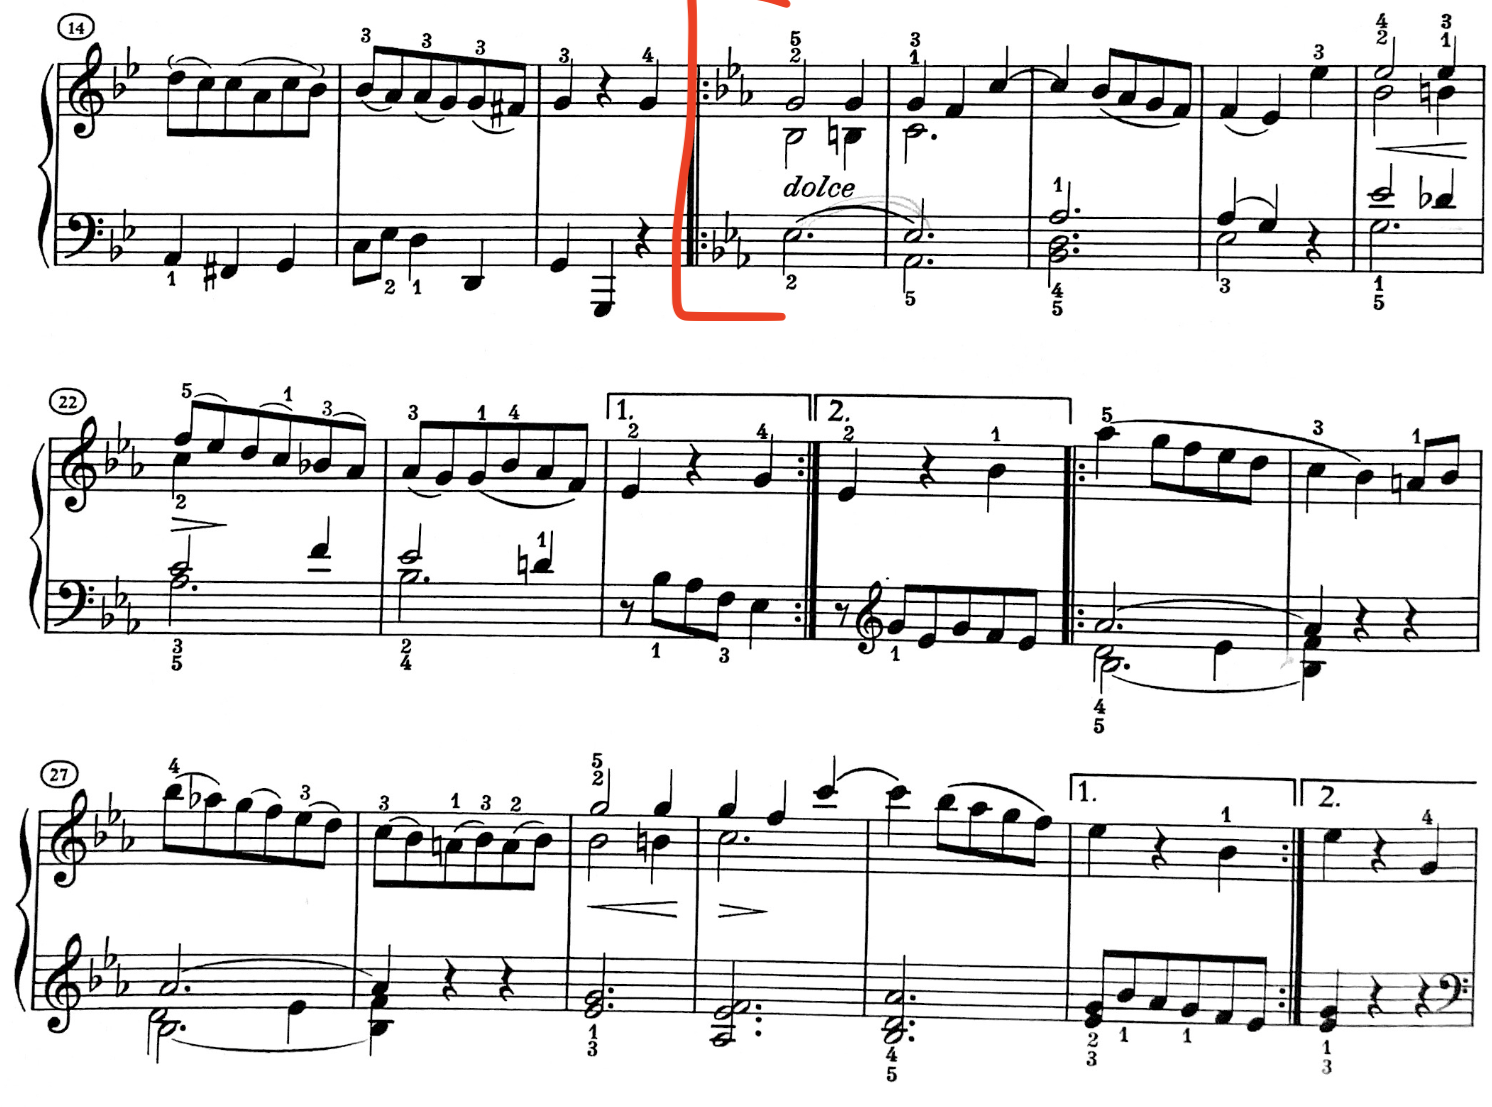
\includegraphics[width=0.5\textwidth]{figures/beethoven-b-section.jpg}
	\caption{The B section, in Beethoven's \textit{Eleven Bagatelles}}
	\label{fig:beethoven-b-section}
\end{figure}

As previously mentioned, in the ternary form, each section--the A, B, and A`--is able to stand on its own. The B section will provide a strong contrast with the A and A` sections which surround it, in theme and tone. For this B section, Beethoven modulates to the key E\musFlat{} Major. The sudden key change from G Minor to related key E\musFlat{} Major alerts listeners to understand that this is a new section. Other differences in the B section from the first A section include a difference in the section's articulation and harmony. With articulation, as seen in Figure \ref{fig:beethoven-b-section}\autocite{Henle_1978} and bracketed in red, there are no staccatos in this section. Instead, the section flows together more than the A section. It sound much more lyrical, and connected. Opposed to the left-hand in the A section, the B section's left-hand plays more block chords, and this leads to an overall greater depth in the section's sound. These left-hand notes are also played in a lower octave than the notes that were played in the A section. 

In bar thirty-seven, there is a return to the material which appeared in the A section. This marks the A` section. However, instead of being a strict restatement of all the material of the first A section, Beethoven repeats the material with variation. This is defined as a phrase of music which is a varied version of an original theme. Some variations may follow this original theme very closely, and others may be more original, only referencing the original theme through harmonies or melodic references.\autocite{Kennedy_Kennedy_Rutherford-Johnson_2013b} In the A` section, while there a return to the material that was introduced in the first A section, the material is also now a variation. The first A section's melody is still intact, but it is now more \say{hidden}, with the melody notes sounding on every second eighth note, as seen in Figure \ref{fig:beethoven-a-prime-melody-variation}\autocite{Henle_1978}. Beginning in beat three of bar forty-four, the melody sounds on every second eighth note. The shape and melody of the original A section is still there, only less obvious.

\begin{figure}
	\centering
	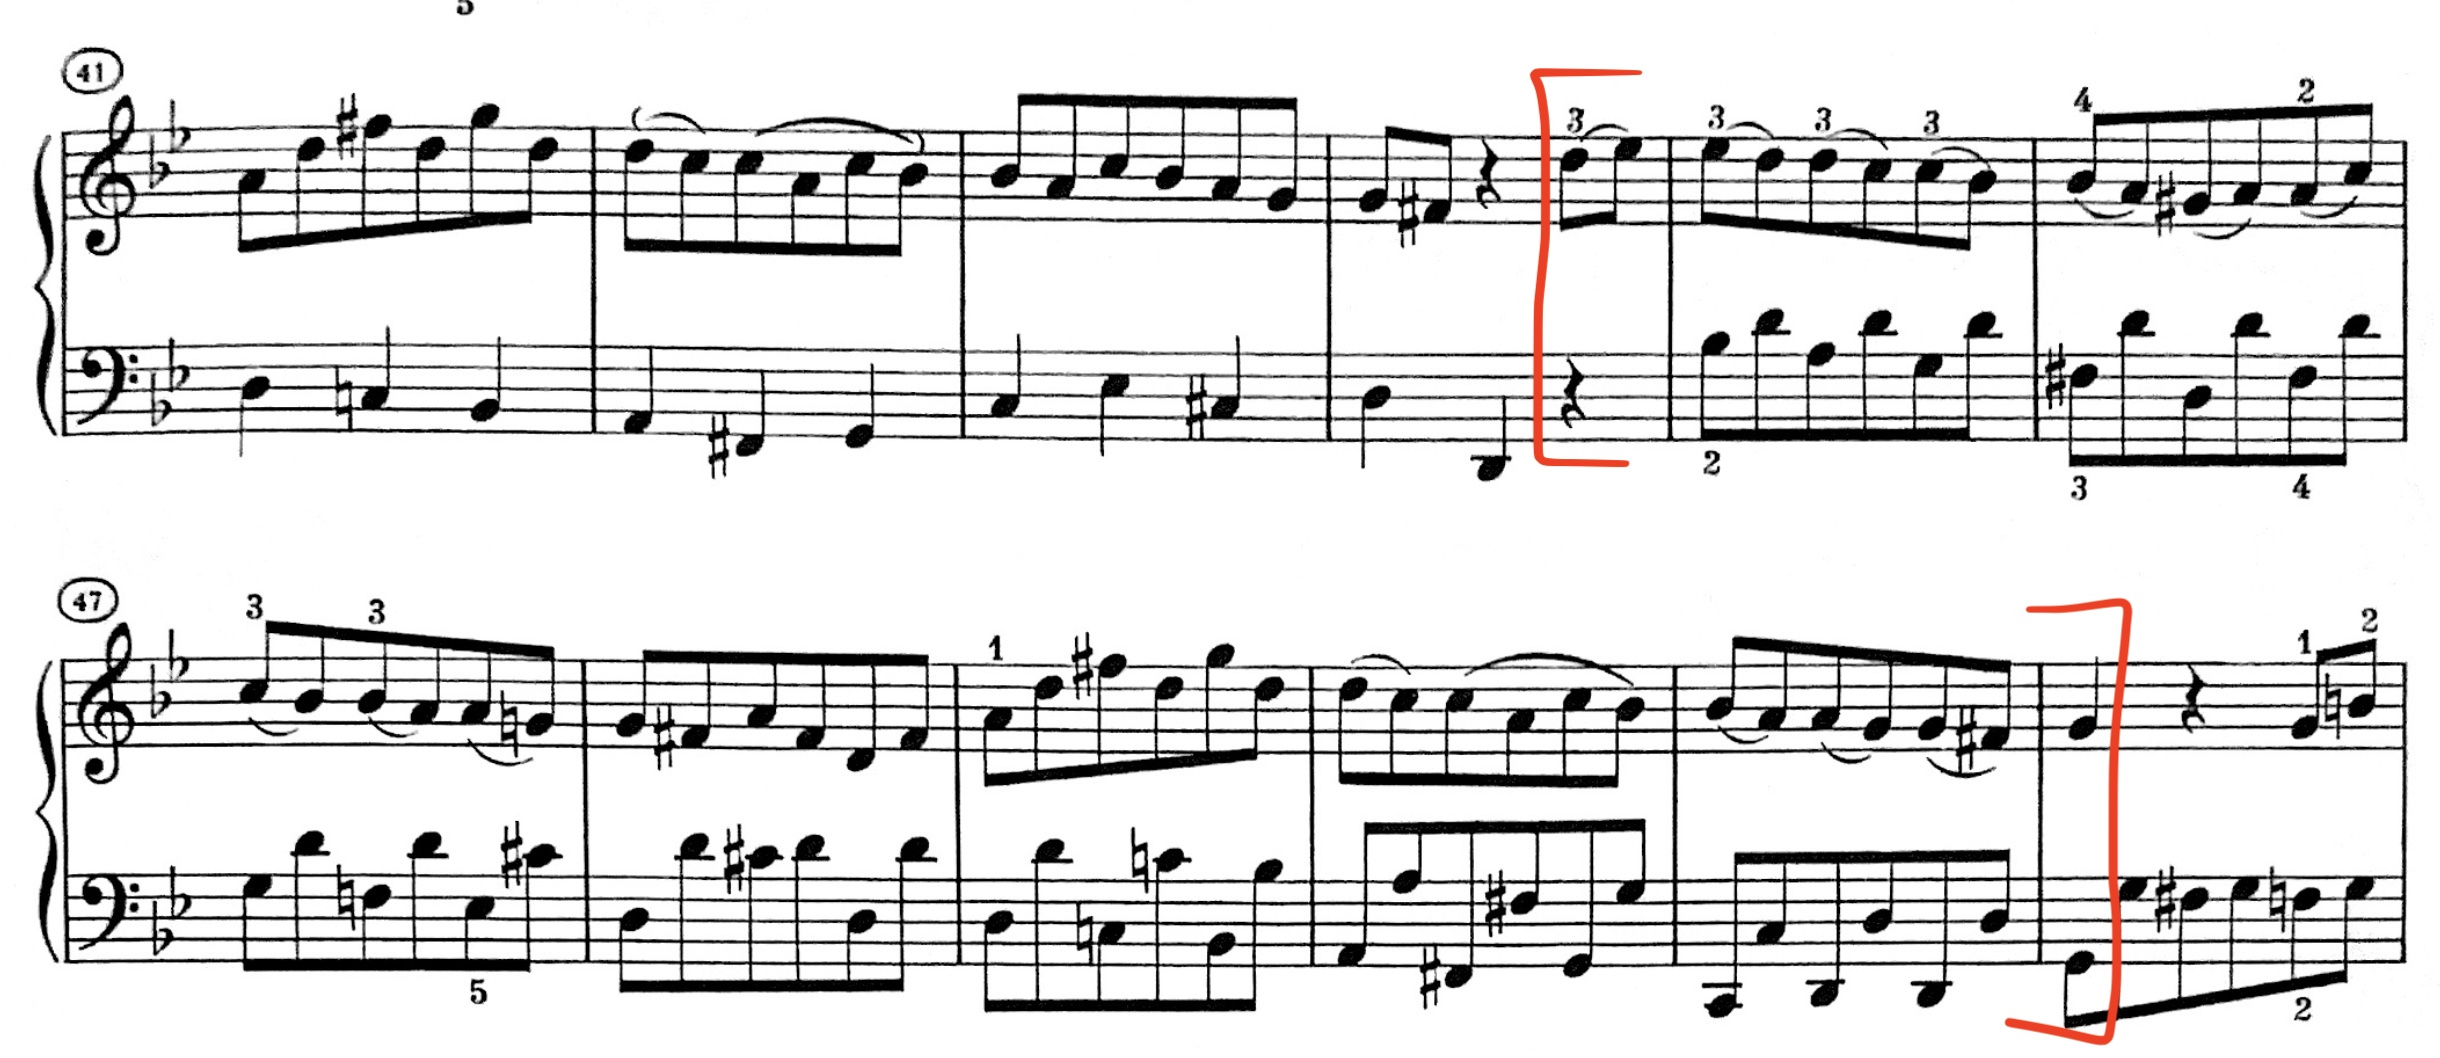
\includegraphics[width=\textwidth]{figures/beethoven-a-prime-melody-variation}
	\caption{The variation of the original melody in the A` section of Beethoven's \textit{Eleven Bagatelles}}
	\label{fig:beethoven-a-prime-melody-variation}
\end{figure}
\chapter[Chopin and Prelude, Op. 28, No. 15]{Frédéric Chopin - \textit{Prelude, Op. 28}, No. 15, the ``Raindrop'' Prelude (1838)}

Fryderyk Chopin (1810-1849) was a composer during the Romantic period (generally known to be from 1800-1910) who composed primarily for the piano. Born near Warsaw in a section of Poland which was at the time under Russian control, Chopin's clear talents as a musician were clear from an early age. By age seven, he had played his first public concert as a soloist, and had published his first piece. Over the course of years, his pieces would evolve to have a defined Polish character. In 1830, Chopin began touring through Germany and Italy, to gain an international reputation as a performer and composer, and settled in Paris, France in 1831. By this point, Chopin had already mostly reached fully compositional maturity. Four genres generally attributed to Chopin, the mazurka, étude, waltz, and polonaise, had matured by then, as Chopin had begun writing these in the 1820s\autocite{Burkholder_Grout_Palisca_2014}. The étude, a genre heavily associated with both Chopin and fellow Romantic-era composer Franz Liszt, is a piece which is intended to develop technique, or a certain skill on the instrument of choice, and only develops a singular figure through the piece. The other three genres that are known to be \say{Chopin genres} are stylized dances, typically for students, and are idiomatic in both figurations and fingerings\autocite{Burkholder_Grout_Palisca_2014}. Chopin's waltzes evoked the spirit of ballrooms in Vienna, but the mazurkas and polonaises are infused with Polish character. The polonaise is a type of courtly, and aristocratic dance, in $\frac{3}{4}$ time, also marked by a rhythmic figure of one eighth note and two sixteenth notes on beat 1. The mazurka is a Polish folk dance, and in the time of Chopin, had become an urban type of ballroom dance, popular amongst those in high society in both Paris and Poland. Similar to the polonaise, the mazurka is in $\frac{3}{4}$ time, with accents on beats 2 and 3, and a dotted figure of some kind on beat 1. Mazurkas also feature a simple accompaniment, especially in the left-hand for piano, and combine four-bar long phrases into periods which alternate in A BA C form. The melody for a mazurka is also important, as it is instrumental in style, rather than vocal in style. This leads to elements of Polish instrumental folk music being prominent, and includes aspects solely found in melodies of instrumental music: large trills, grace notes, large leaps from one note to the next, and slurs to imitate the bowing found in traditional Polish folk songs. If articulated properly, a mazurka would sound uneven in tempo as it allows for ornamentations (such as the \textit{sforzando}, trills, and grace notes) to lengthen in time, and would lead to dancers to be able to execute turns or lifts. 

In the years before 1838, when the Raindrop Prelude was written, there was a brief, albeit interesting, period of Chopin's life. A period of writing, 1837 marked the year in which Chopin crossed paths with George Sand, a novelist later to be Chopin's partner, yet it was not until April 1838 in which they made this pairing official. The pair, along with Sand's children, spent the winter months of 1838-9 in Valldemossa, Majorca, an old Carthusian monastery. Recuperating from an illness and in the midst of a winter storm, Chopin began writing the 24-set preludes\autocite{Samson_2001}. Thus, the title of the fifteenth prelude of this set relates to the rain and stormy weather Chopin weathered while at Majorca, as well as the uncertainty regarding his health.

In 1838, Chopin wrote the set of 24 preludes, Opus 28, of which the fifteenth (simply known as the \say{Raindrop Prelude} is arguably one of the most famous of this set. Structurally, this prelude is in ternary form, with three sections: \textit{ABA}, and a coda. 

\begin{figure}[h]
  \centering
  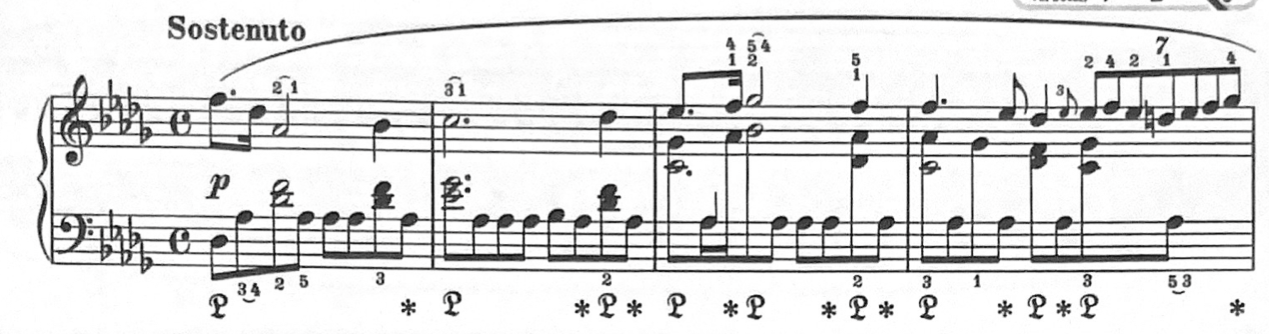
\includegraphics[width=\textwidth]{chopin-a-section-first-four-bars.jpg}
  \caption{The first four bars of Chopin's \textit{Prelude, Op. 28, No. 15}}
  \label{fig:chopin-a-section-first-four-bars}
\end{figure}

The first section, A, is a sweet section, reminiscent of gentle rain, akin to a sprinkle of rain. The delicate nature of this section is shown in the continuous usage of the \textit{piano} dynamic, as in Figure \ref{fig:chopin-a-section-first-four-bars}\autocite{Hansen_1973}. So, the performer playing this piece will play this section, as well as its related A' section, as the most expressive of the piece. As implied in bars 3-4 of Figure \ref{fig:chopin-a-section-first-four-bars}\autocite{Hansen_1973}, this typically becomes an interpretation in which there is a consistent usage of \textit{rubato}\autocite{Cole_Schwartzb}\footnote{A common practice in Romantic-era compositions. It involves taking a part of the duration of one note, and then giving it to another note. The performer is tasked with tastefully stretching, slowing, or hurrying the tempo, to their discretion. This gives the performer the greatest amount of flexibility and emotion available to interpret the piece.} and gradual crescendos and decrescendos to and from mezzo piano (medium loud). This is best seen when the piece in bars 3-4 ascend, peaking on the note G, and then descend, to a temporary low of D. This rise to G and subsequent fall to D will typically be played as a crescendo as the performer reaches the note G, and then a decrescendo back to \textit{piano} as the performer approaches the note D. The titular raindrop that this piece is named after is easily heard within the first three notes played in this piece and section: F, D\musFlat{}, and A\musFlat{}, outlining the piece's tonic key of D\musFlat{} Major. This phrase of three notes repeats again in other places in section A and A', as the raindrop motif, signifying the raindrops falling, and giving the section a melody which is cantabile and smooth. This section also features a repeated-note motif of the A\musFlat{} which is found in the left-hand, as in Figure \ref{fig:chopin-a-section-first-four-bars}\autocite{Hansen_1973} and many other places throughout A and A' sections. The raindrop motif stands out more against the background hum, or the sounds of other raindrops falling in tandem, which the left-hand's pedal point provides. The two motives here provide a texture which is entirely homophonic in this section. The texture solely consists of the right-hand melody, and the raindrop motif, and the left-hand's accompaniment, with the pedal point motive. This causes the section to sound thin in texture and timbre, as the right-hand provides its melody through the use of broken chords, and the left-hand provides a pedal note. Beyond the simplistic homophonic. texture, this section also contains tasteful ornamentation, featuring the use of rubato and other rhythmic ornamentation, among others, as shown by Figure \ref{fig:chopin-a-section-examples-ornamentation}\autocite{Hansen_1973}. At the end of the A section, there is a key change to the relative minor key of C\musSharp{} Minor, D\musFlat{} Major's relative minor key. This becomes the B section's tonic key.

\begin{figure}
  \centering
  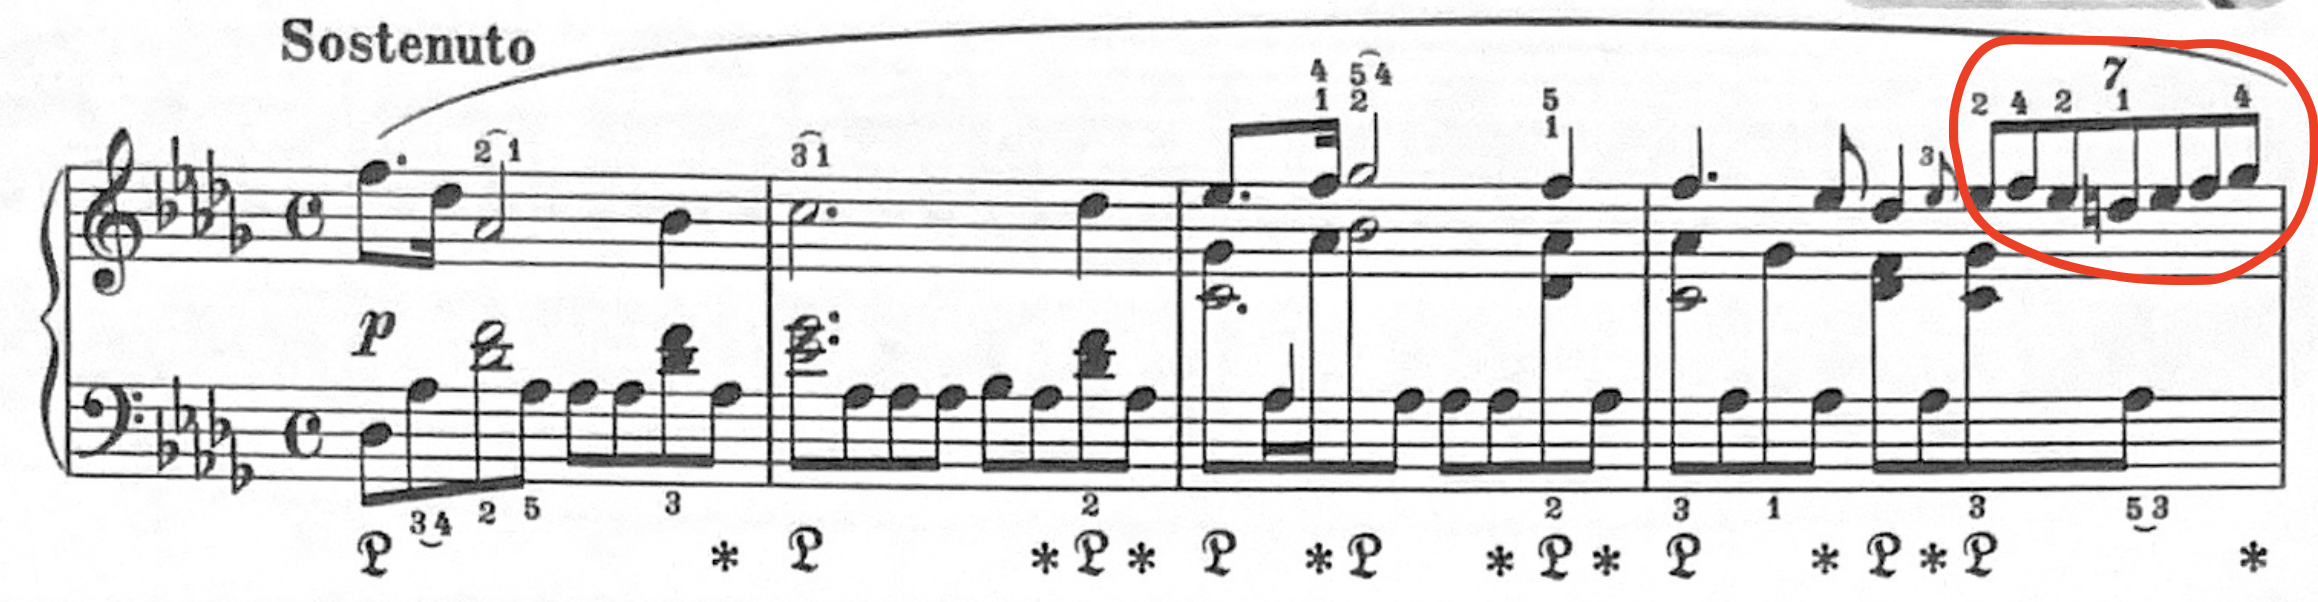
\includegraphics[width=\textwidth]{chopin-a-section-seven-note-run.jpg}
  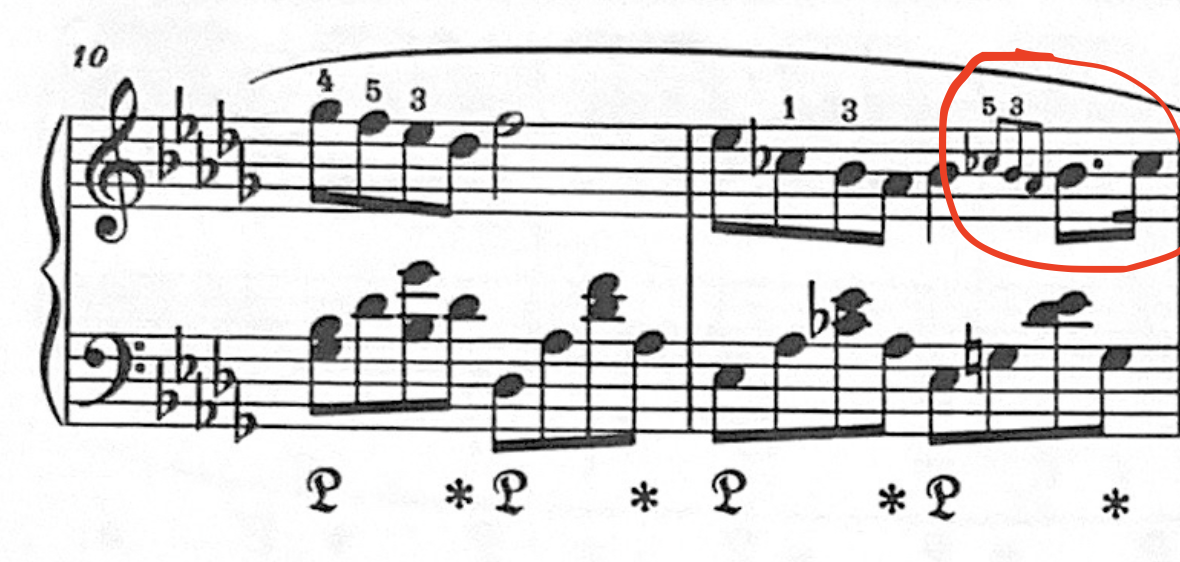
\includegraphics[width=\textwidth]{chopin-a-section-triplet-grace-note.jpg}
  \caption{Several examples of ornamentation, in Chopin's \textit{Prelude, Op. 28, No. 15}}
  \label{fig:chopin-a-section-examples-ornamentation}
\end{figure}

\begin{figure}
  \centering
  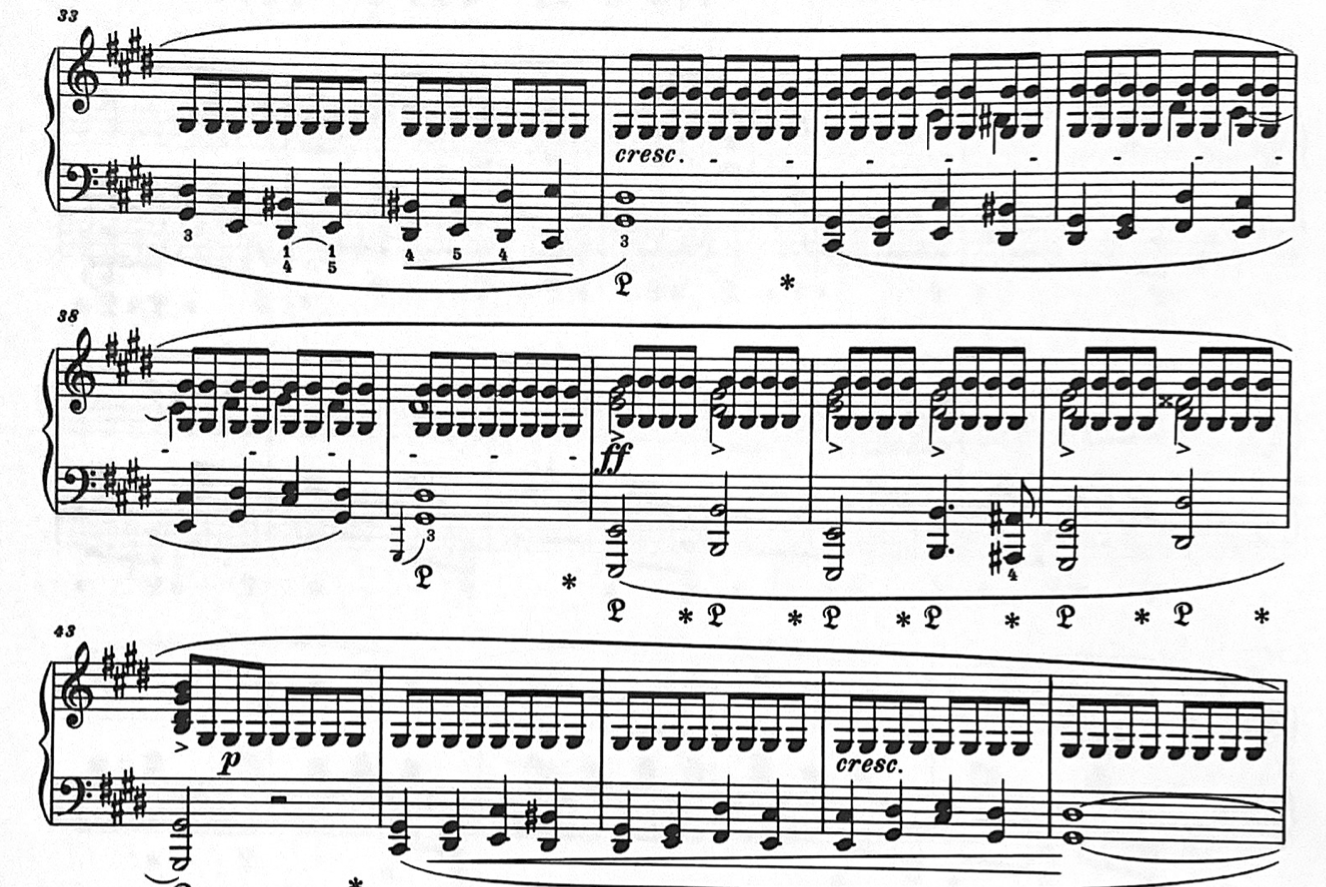
\includegraphics[width=\textwidth]{chopin-b-section-crescendos.jpg}
  \caption{The changes in dynamics, in Chopin's \textit{Prelude, Op. 28, No. 15}}
  \label{fig:chopin-b-section-crescendos}
\end{figure}

\begin{figure}
  \centering
  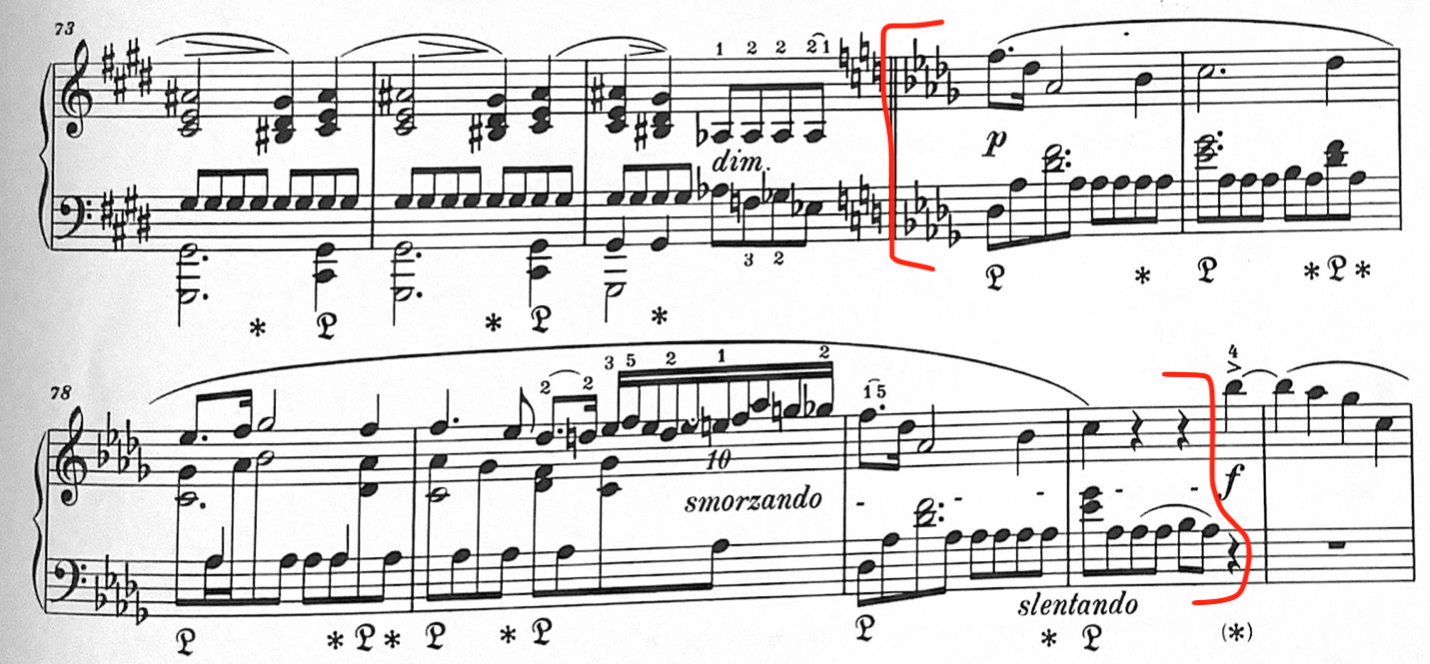
\includegraphics[width=\textwidth]{chopin-a-prime-section-ornamentation.jpg}
  \caption[Ornamentations in A', Chopin's \textit{Prelude, Op. 28, No. 15}]{The various ornamentations in the A' section of Chopin's \textit{Prelude, Op. 28, No. 15}}
  \label{fig:chopin-a-prime-section-ornamentation}
\end{figure}

\begin{figure}
  \centering
  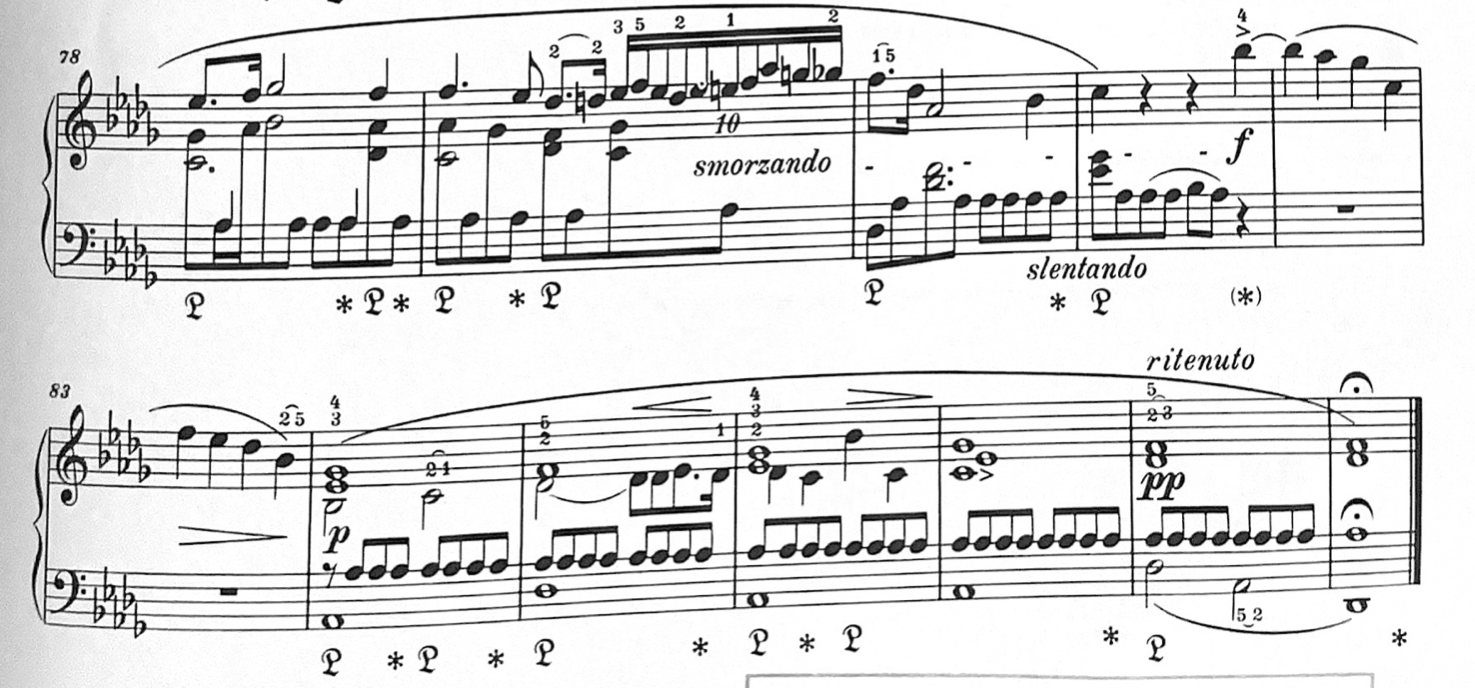
\includegraphics[width=\textwidth]{chopin-coda.jpg}
  \caption{The coda, Chopin's \textit{Prelude, Op. 28, No. 15}}
  \label{fig:chopin-coda}
\end{figure}



The B section is a high contrast to section A in character and tone. With the key change to C\musSharp{} Minor, the pedal note of A\musFlat{} turns into G\musSharp{}, and tension is introduced in this section. While section A's texture was a homophonic one, this section's texture is much more chordal, with chords featured in both hands, and also contains notes which are generally lower in pitch. Additionally, the repeated note motif is now in the right-hand, as it plays the note G\musSharp{}, in Figure \ref{fig:chopin-b-section-crescendos}\autocite{Hansen_1973}, creating a sort of ``inverted'' pedal point. The melody then shifts to the left-hand. As the section goes on, crescendos are used to build additional tension (see Figure \ref{fig:chopin-b-section-crescendos}\autocite{Hansen_1973} for reference, for example) as the dynamics increase from \textit{sotto voce} to \textit{fortissimo} ( \say{very loud}). The section begins \textit{sotto voce} (``under the voice'', which has similar meaning to \textit{piano}), and gradually builds with crescendos\footnote{Figure \ref{fig:chopin-b-section-crescendos}}\autocite{Hansen_1973}. As the tension builds, the left-hand also adds slurs as ornamentation, adding a legato effect to the notes which also contributes to the rising tension. Once the dynamics peak at \textit{fortissimo}, the volume drops to \textit{piano} and repeats the section again. Dynamics are the primary tool used by the performer to add their interpretation and expression to the piece in this section, and the \textit{fortissimo} is used to great effect when the crescendo builds, and is at its highest when we arrive at the chords of E Major and B Major.

The return of the A section, although a modified version, returns the original melody of the first A section. It return \textit{piano}, and is also marked \textit{smorzando} (``dying away'') to signify the intended ending in \textit{pianissimo} (very soft). The first A section's tonic key of D\musFlat{} Major returns, and so does a majority of the ornamentation decisions, including rubato, and other decorations which are explored more deeply, as in Figure \ref{fig:chopin-a-prime-section-ornamentation}\autocite{Hansen_1973}. However, we only hear the first eight bars of this second A section, as Chopin includes a coda to finish the piece.

This coda (or more accurately, codetta, a short coda) finishes the prelude. As seen in Figure \ref{fig:chopin-coda}\autocite{Hansen_1973} and marked in red brackets, there are elongated quarter notes which descend, played in \textit{forte} (loud), to add a sense of both intensity and delicacy to the ending. In the third full bar of the coda, the pedal point is reintroduced, this time as A\musFlat{}, played in the right-hand. It, like its role in the first A section, is like that of falling raindrops, serving as a background sprinkle for this ending. The coda ending is marked with the word \textit{ritenuto}\autocite{Cole_Schwartza}, to indicate the sudden slowing of the tempo, almost an extreme slowing of the tempo. With the \textit{ritenuto}, it is a clear ending to this prelude, and is akin to the ending of a rainstorm, in which the rain clears up.

\section{...But He's Supposed to be Dead!}\label{section:chopin-interpretation}

Chopin wrote this prelude during one particularly brutal winter, in Valldemossa, Majorca. This prelude is number fifteen of the twenty-four set of preludes. As its title ``Raindrop'' suggests, the fifteenth prelude relates to the rain and stormy weather which Chopin was subject to during his time alone in Majorca. There was uncertainty regarding his health, and this is clearly seen in all aspects of the piece.

In the very first measure of the piece, in the A section, we note two things. First, that Chopin has set the dynamic marking of the piece's beginning to be \textit{piano}, with the right-hand melody meant to be played smoothly. Second, that the first three notes played in the right-hand, as in Figure \ref{fig:chopin-a-section-first-four-bars}\autocite{Hansen_1973}, emulates the sound of raindrops falling. There is the rhythm of a dotted eighth note, followed by a sixteenth note and a half note. This places the sound of the falling rain at the center of the piece, as a melodic motif that a listener can easily decipher. Thus, I play it out, fading the left-hand harmony into the background, as this is the central motif to the entire prelude. The left-hand harmony becomes the low murmur of rain hitting the roof of a home, and the soprano notes (the highest notes which sound in the right-hand) become more pronounced, as the melody rises and falls. Other dynamic markings which Chopin includes in the A section of this piece are also instrumental to my performance of this section as warm and lulling in nature. As the melody line in the right-hand rises and falls, I match each peak and dip in melody with its appropriate dynamic contrast; when the melody rises and peaks at the note G (as it does in Figure \ref{fig:chopin-a-section-first-four-bars}\autocite{Hansen_1973}), I increase the dynamic of the melody to its loudest, and do the same with the lowest note D, decreasing my dynamic to its lowest. Additionally, as mentioned, while I choose not to place emphasis on any of the notes below Middle C, I play the left-hand as warm and as full as I can, to encapsulate the nature of a violent wind and rainstorm happening outside, the way Chopin might have heard it. It is easy to play the melody out against a soothing backdrop of rain patter, as it acts as a pedal point through which the listener can focus on other sounds instead.

Beyond the literal representation of the windstorm happening to Chopin while at the Carthusian monastery he stayed at in 1838-9, the A (and later, A') section is also meant to represent Chopin's fear of death and dying alone without his loved ones near. As in Figure \ref{fig:chopin-a-section-examples-ornamentation}\autocite{Hansen_1973}, in addition to the raindrop motif frequently reoccurring in various iterations, there is also the use of other ornamental tools which I use to highlight Chopin's unease with facing his mortality. There is a clear fear of death, which I present through placing greater emphasis and rubato on three-note phrases which include a dotted eighth note and sixteenth note. In addition, there are also several passages, such as in measure 11 of Figure \ref{fig:chopin-a-section-examples-ornamentation}\autocite{Hansen_1973}, in which triplets, and three- to seven-note grace notes, allude to the uncertainties regarding death. Within phrases which contain either three-note grace notes or seven-note grace notes, I play these quicker, with a slight bounce to them. This again emphasizes the intense fear of death Chopin had, as well as the unknown regarding aspects of medicine and sickness in the seventeenth century.

As the A section transitions into the B section, there is a change in texture, timbre, and overall sound quality. I follow this transition in sound, placing greater emphasis on the left-hand's bass notes, and bringing the dynamic level of the left-hand harmony to equal that of the right-hand. When the B section begins, as in Figure \ref{fig:chopin-b-section-crescendos}\autocite{Hansen_1973}, the dynamic volume is still piano, and the right-hand plays either single notes, octaves, or a combination of both. I maintain the same steady increase and decrease in dynamic volume as I did in the A section, as I begin the B section playing \textit{piano}, and slowly yet dramatically increase the volume as the crescendos note. Chopin had far more anxieties about his health, which comes across in this section. The first two measures of the B section start off tame in comparison to the latter half of the section, as the right-hand creates a pedal point on the note G\musSharp{}, while the left-hand plays a \textit{dyad}, or a two-note chord. These anxieties slowly fester within Chopin, and become ``louder'' in volume, as does the section's dynamics, with the five-measure long crescendo, peaking at a rambunctious and resounding \textit{fortissimo}. Within the music, there is little action, but I sound it to appear at least twice as complex. With the left-hand slowing in its action (from dyad quarter notes to the octave half notes, with occasional dotted quarter notes and eighth notes), the right-hand melody gains movement. Between measures 36-38, on beats 3 and 4 in Figure \ref{fig:chopin-b-section-crescendos}\autocite{Hansen_1973}, the right-hand octaves also feature two slurred quarter notes. These change to become dyad half notes, which sound under the right-hand's octaves. 

It is here, in measures 40-42, where the emotional climax of the piece lies. On beat 1 of bar 40, the left-hand plays a loud and dramatic half note, holding on the note E, while the right-hand plays four eighth note octaves on B, while also holding a half note dyad on E and G\musSharp{}. It is heavy, and intense, and provides a sharp contrast to the material treated in both the A  section, and the first seven bars of the B section. The rain is coming down much harder, and the wind is howling, which I emulate through the half notes that sound in the right-hand. These half notes are noticeable, but do not draw the listener's attention away from the octaves the right-hand plays. Once the left-hand introduces its octaves to be played in bar 34 in Figure \ref{fig:chopin-b-section-crescendos}\autocite{Hansen_1973}, there is a certain dramatization of the acceptance of death Chopin goes through. In the dynamic level of \textit{fortissimo}, there are accents on beats 1 and 3 (Figure \ref{fig:chopin-b-section-crescendos}\autocite{Hansen_1973}) and the half notes in the left-hand are complemented by the right-hand's half notes, creating a sound akin to the resounding Castillo gong in the Carthusian monastery. As the half notes are being held to their full duration, and I play the right-hand's octaves on top of the half notes, I emphasize the nature of the half notes, similar to the gong sounding in a monastery. The phrase in measures 40-42 portray Chopin's fear about death, as the gong sounding gets louder and also somehow closer to the listener, as it comes closer to him. This gong sound comes back later in the section, and alternates in thematic material treated, between the build-up of the rain and the wind, the dynamic marking returns to be \textit{piano}, and the left-hand resuming its prior movement. 

When the A section returns (in the form A'), bracketed in red in Figure \ref{fig:chopin-a-prime-section-ornamentation}\autocite{Hansen_1973}, the treated melodic material is mostly the same, except for ornamental changes. The rain and wind have decreased in intensity, and the difference between the end of the B section and the beginning of the A' section is stark. While the last few measures of the B section (bars 73-75 in Figure \ref{fig:chopin-a-prime-section-ornamentation}\autocite{Hansen_1973}) were dramatic, rambunctious, and referred to Chopin's uncertainty and fear about his own mortality, the beginning of the A' section is the calm reprieve for both the listener and Chopin. The first major change between the A' and the A section is the ten-note long sixteenth note phrase in bar 79 of  \ref{fig:chopin-a-prime-section-ornamentation}\autocite{Hansen_1973}, indicating the rain has not fully finished falling yet, nor has Chopin accepted the possibility of his death. 

The coda of the A' section, in Figure \ref{fig:chopin-coda}]\autocite{Hansen_1973}, is when I emphasize the finality that Chopin has, accepting the calm after the storm, as well as the possibility of his death. In beat 4 of bar 81 through the bracketed passage in red of Figure  \ref{fig:chopin-coda}]\autocite{Hansen_1973}, the left-hand harmony disappears, as the right-hand sounds alone for the first two measures. Played \textit{forte}, I interpret this to not only literally be the calm after the storm, but also a figurative rainbow which appears after the rain has stopped, and the sky has cleared. The only sounds for the first two full measures of the coda contain quarter notes, slurred into one another, and played \textit{forte}. It is the sudden appearance of a rainbow, like those that happen in the media, and which brightens the sky and clears Chopin, and the listener, of fears regarding death. Instead, both Chopin and the listener are transported into an acceptance of the inevitable, and are able to see the beauty in the calm. This acceptance is not overdramatized by my performance, as I keep the dynamic level of bar 84 to the end at a \textit{piano}, and let the melody and harmony lines perfectly balance each other. The whole notes in the left hand ground the right-hand's melody, while the eighth notes in the left-hand emphasize the acceptance of death and the beauty of the rainbow, and do not overstate its importance. The addition of the pedal, starting in bars 84 (Figure \ref{fig:chopin-coda}\autocite{Hansen_1973}) also adds to the air of acceptance and inner peace, as the coda ends with the word \textit{ritenuto}. The extreme slowing of tempo and shift to a dynamic of \textit{pianissimo} symbolizes this recognition and compliance, as it ends with satisfied whole note dyads in both hands, and a fermata elongating the notes' durations.
%
%Could also tie in idea of rain and the literal rain interpretation with the intense fear of death \& eventual acceptance with the calm after a heavy rain \& stereotypical rainbow afterwards
\chapter[Tchaikovsky's June: Barcarolle from \textit{The Seasons}, Op. 37a]{Pyotr Ilyich Tchaikovsky - June: Barcarolle from \textit{The Seasons}, Op. 37a (1875)}

Pyotr Ilich Tchaikovsky (1840-1893) was a leading Russian composer during the nineteenth-century. Born in Votkinsk, Russia, Tchaikovsky moved with his family several times, including to Moscow and St. Petersburg, as his father searched for a job\autocite{Burkholder_Grout_Palisca_2014}. This did not dissuade Tchaikovsky from attempting to pursue a serious musical study, as he studied at the St. Petersburg Conservatory between 1862-1865, and then left to Moscow, where he received a teaching position at Moscow's Conservatory. During his time at the Moscow Conservatory, he composed his work \textit{The Seasons}, twelve character pieces for piano. A character piece is a type of program music. Program music is defined as a type of music which tells a story, able to illustrate various literary ideas or evoke pictorial scenes\autocite{Kennedy_Kennedy_Rutherford-Johnson_2013a}, and this definition can be expanded to include all music which attempts to represent some type of extra-musical material or concepts without spoken words\autocite{Scruton_2001}. The term ``program music'' was introduced by Franz Liszt, also the creator of the term \say{symphonic poem}, to describe the most characteristic aspect of program music. He described program music as music which the composer can both guard the listener against the ``wrong'' interpretation of the music, and also direct the listener's attention to the ``proper'' ideas of the piece as a whole or a particular piece of it. Contrasted with absolute music, music without these extra-musical concepts, program music is best characterized by its attempt to depict objects and events, not merely echoing or imitating these. In some cases, these pieces may attempt to literally evoke the scene of some type, with Tchaikovsky does to excellent effect with his June Barcarolle from \textit{The Seasons}. A character piece is designed to convey a specific allusion, atmosphere, mood, or scene, without text, stage action, or other program assistance\autocite{Temperley_2011}. The Romantic era (during the nineteenth-century) encouraged literary influences in music, and nationalism of the time led composers, including Tchaikovsky, to evoke the folk music of various nations and ethnic groups. Tchaikovsky did this in his music by combining his Russian heritage with influences from Italian opera, French ballet, and Germany symphony and song, music similar to program music \autocite{Burkholder_Grout_Palisca_2014}.

Each piece in \textit{The Seasons} is of a different month of the year in Russia. The month of June is written in the style of a barcarolle. This is a song written in $\frac{6}{8}$ or $\frac{12}{8}$ time, typically sung by Venetian gondoliers, and has an accompaniment which suggests the rocking of a Venice gondolier\autocite{Latham_2011b}. Within the June barcarolle, there is a slight deviation from the typical barcarolle piece. The piece is written in G Minor, and has an ABA form. Within the A section in Figure \ref{fig:t-first-three-lines}, we notice that this piece is actually in $\frac{4}{4}$ instead of the usual $\frac{6}{8}$ or $\frac{12}{8}$ time. This opening is marked as \textit{Andante cantabile}, or ``slowly sing'', to ensure the performer understands the sensitivity that must be brought to perform this piece. The time signature of $\frac{4}{4}$ and tempo marking \textit{Andante cantabile} gives a sense of pace, as well as the necessary combination of correct rhythm--as the Venetian gondolier ``sings''--and the treatment of the right-hand's melody line. In the first two lines of the barcarolle, a dactylic (defined as a metrical pattern referring to a rhythm in which one strong syllable or beat is followed by two unstressed, or not strong, or short syllables or beats)\autocite{Cambridge_University_Press_Assessment} pattern emerges, as clearly seen by Figure \ref{fig:t-first-three-lines}\autocite{Henle_2002}. Here, there is a clear long phrase which starts the dactylic pattern in bar two. The second beat of four through to the first three beats of bar 6 finish the first set of the dactylic pattern. This pattern repeats, in the last beat of bar 6 through to the first three beats of bar 12. This twelve-bar phrase could form some type of period, ending of the first phrase group in the middle of bar 6 differs slightly from the ending of the second phrase group in the middle of bar 12. Thus, there is an atypical form of the traditional period in the first twelve bars of the piece, found bracketed in red in Figure \ref{fig:t-first-three-lines}\autocite{Henle_2002}. 

\begin{figure}[h]
  \centering
  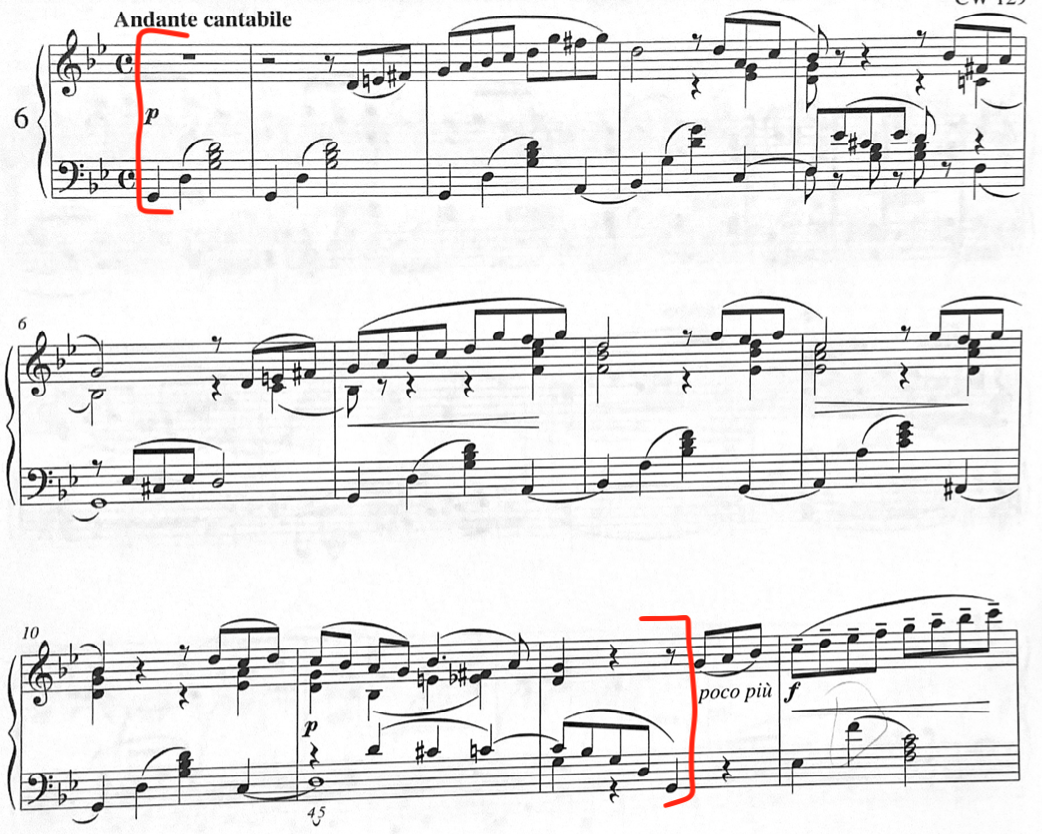
\includegraphics[width=0.5\textwidth]{t-first-three-lines.jpg}
  \caption{Pyotr Ilyich Tchaikovsky, The Seasons, \textit{June: Barcarolle}, mm. 1-13}
  \label{fig:t-first-three-lines}
\end{figure}

Additional stylistic choices to create necessary sensitive and delicate sound, akin to physically being on a Venetian gondola and hearing the water and boat move, involve what is notated in Figure \ref{fig:t-a-section-style-choices}\autocite{Henle_2002}. First, there are several instances of a change in dynamics, with several crescendos and decrescendos marked, along with a \textit{piano} and \textit{forte} to obtain the right level of volume and balance from a performer. Specific to these measures is also the dynamic marker \textit{poco piú} (a marking meaning ``little more''), signifying a crescendo before a crescendo. The phrase peaks in bar fourteen on note F, and decrescendos down as the right-hand approaches the note D. Other increases and decreases to volume follow through to the remainder of the A section, with the \textit{diminuendo} (a smooth decrease in volume) marker being the only other dynamic marker of note in the section.

\begin{figure}[h]
  \centering
  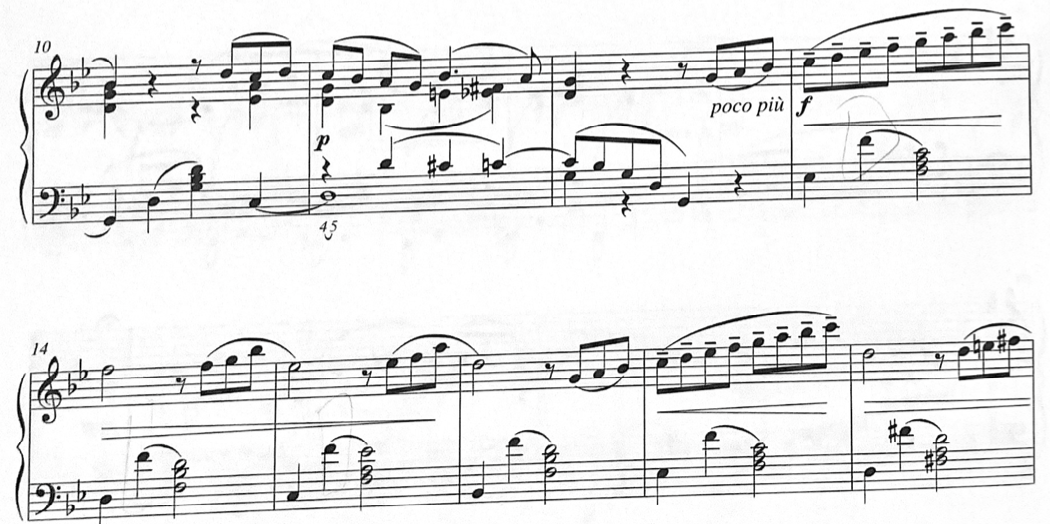
\includegraphics[width=0.5\textwidth]{t-a-section-style-one.jpg}
  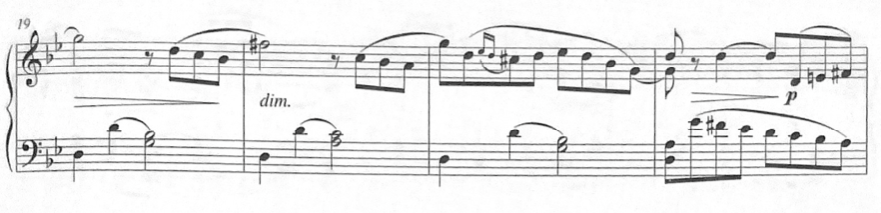
\includegraphics[width=0.5\textwidth]{t-a-section-style-two.jpg}
  \caption{Pyotr Ilyich Tchaikovsky, The Seasons, \textit{June: Barcarolle}, mm. 10-22}
  \label{fig:t-a-section-style-choices}
\end{figure}

\begin{figure}
  \centering
  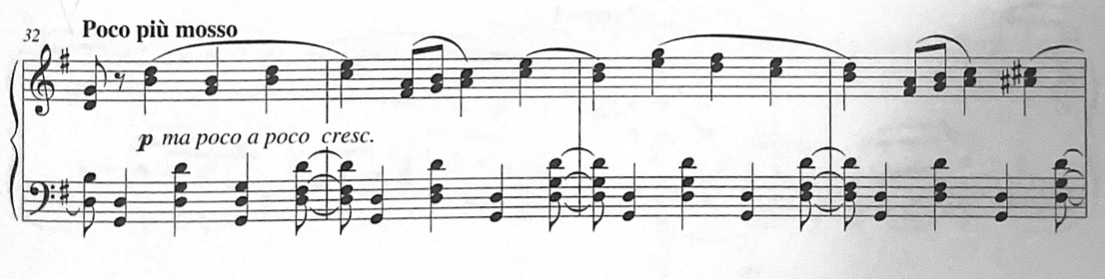
\includegraphics[width=\textwidth]{t-b-section-bars-32-35.jpg}
  \caption{Pyotr Ilyich Tchaikovsky, The Seasons, \textit{June: Barcarolle}, mm. 33-34}
  \label{fig:t-b-section-bars-32-35}
\end{figure}

\begin{figure}
  \centering
  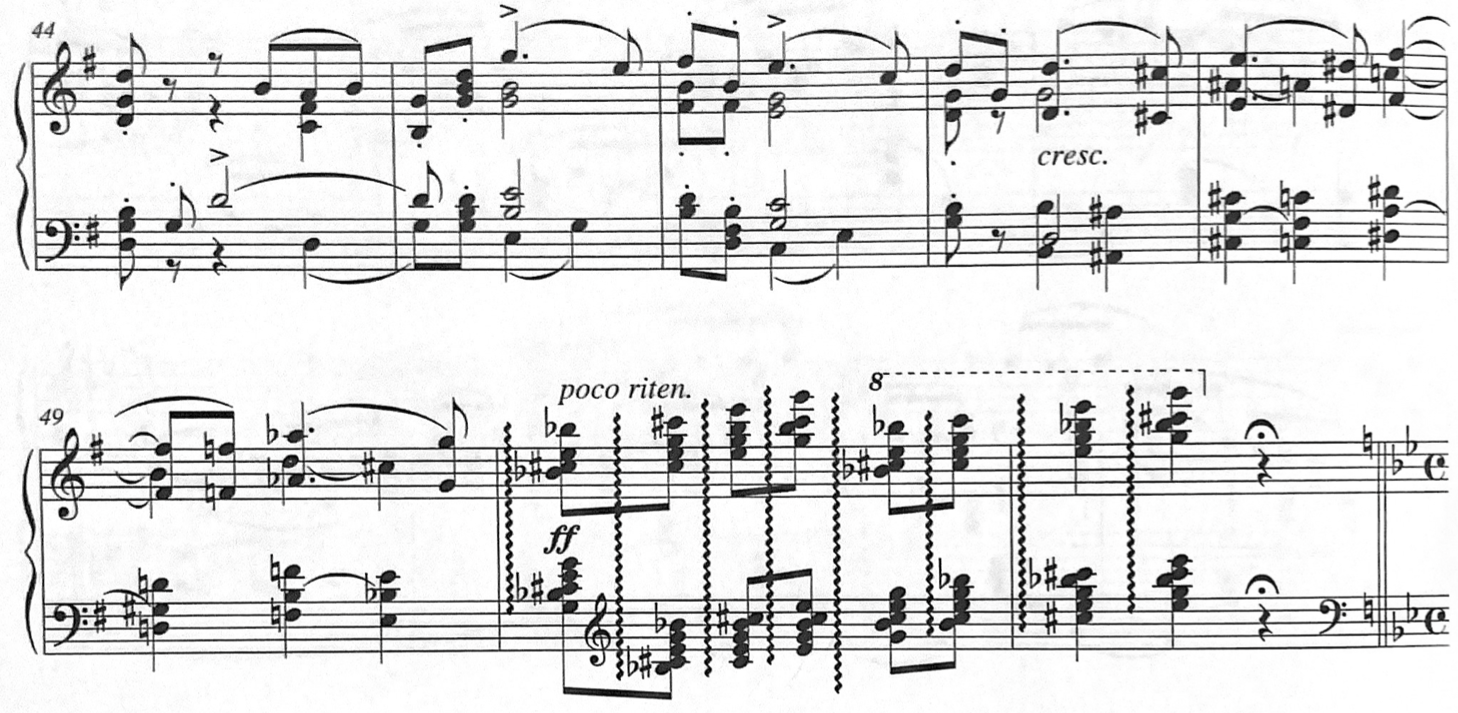
\includegraphics[width=0.7\textwidth]{t-b-section-bars-44-51.jpg}
  \caption{Pyotr Ilyich Tchaikovsky, The Seasons, \textit{June: Barcarolle}, mm. 44-51}
  \label{fig:t-b-section-bars-44-51}
\end{figure}


In the B section, the Venetian song continues, further immersing the listener into the song. The start of the section, as in Figure \ref{fig:t-b-section-bars-32-35}\autocite{Henle_2002}, begins with the tempo marking \textit{poco piú mosso} (roughly translating to ``a little bit faster''). It begins \textit{piano}, and as notated by the \textit{ma poco a poco crescendo}, the dynamic of the piece gradually increases slowly, until it reaches a peak at bar forty. The performer plays at \textit{forte}, indicating an increase in intensity within the Venetian gondolier's song, and a possible rockier nature to the gondola itself. This intensity is maintained through much of the section. Between bars 44-51, as in Figure \ref{fig:t-b-section-bars-44-51}\autocite{Henle_2002}, there are several other rhythmic and harmonic notations which the performer must keep in mind as well to maintain the necessary level of intensity and dramatization of the gondolier's song. Differently accented notes along with slurring certain lines contribute to the overall feeling of unsteadiness while the gondola floats its way down the Venice canal. Bars 44-46 are examples, as there are notes in both hands which begin as accented notes, and are followed immediately by slurred notes in short two-note phrases. Along with the staccato notes spread out in this figure, as well as the crescendo found in bar 47, the paddles of the gondola are heard in the background. The gondolier's singing is prominent above the sounds of the water in the canal and the rowing of the gondola itself, as the gondolier's singing becomes more dramatic and louder, through bar forty-seven's crescendo, and through to the arpeggiated chords in bars 50-51. The B section ends, with the arpeggiated chords of Figure \ref{fig:t-b-section-bars-44-51}\autocite{Henle_2002} becoming gradually slower with the \textit{poco ritenuto} tempo marking, culminating in a dramatic quarter-note length final note, and an extended quarter-note length rest (this extension is known as a fermata).

Slightly before the return of the A section, there is a brief measure and a half transition section. As in Figure \ref{fig:t-a-prime-beginning}\autocite{Henle_2002}, there is a descent is the harmonic line in the left-hand, with bar 52 to be played in \textit{forte}, and the second beat of bar 53 played in \textit{mezzo forte}. This transition section reduces the intensity and high-energy that was found in the B section, moving it back to the gentle sensitivity of the A section. This is helped by the three note slur which starts this section, and the fermata over the two tied quarter notes which ends the section. Programmatically, the highest peak of the Venetian gondolier's song is over. The block chords of the B section give way for the broken chords style in the A section, with block chords in the transition section only signifying the transition to the A section. The gondola is able to continue on its journey, gentling floating down the Venice canals with the help of the gondolier.

\begin{figure}[h]
  \centering
  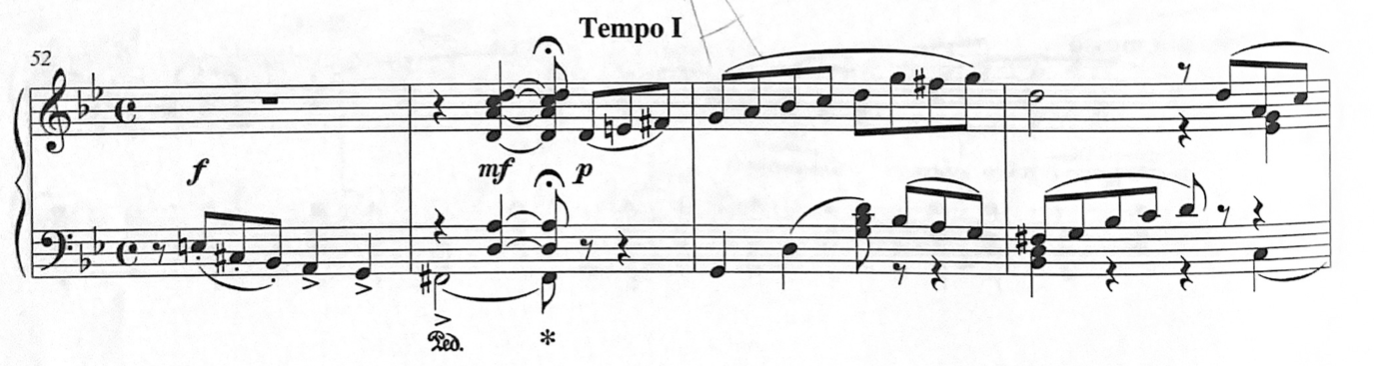
\includegraphics[width=0.5\textwidth]{t-a-prime-beginning.jpg}
  \caption{Pyotr Ilyich Tchaikovsky, The Seasons, \textit{June: Barcarolle}, mm. 52-55}
  \label{fig:t-a-prime-beginning}
\end{figure}


Finally, the A' begins, featuring a return of many of the material that was treated in the first A section. The tempo of the piece goes back to \textit{Tempo I}, the A section's tempo and the original tempo of the piece. The dactylic nature of the A section also returns in A', and as in Figure \ref{fig:t-a-prime-beginning}\autocite{Henle_2002}, the Venetian gondolier's song has lessened in intensity and energy, with the listener only vaguely aware of the left-hand's slurred motion which simulated the rocking of the gondola, and the gondolier slowly bringing the song to an end. Towards the end of the A' section, there is a return of the block chords which featured heavily in the B section, as in Figure \ref{fig:t-a-prime-ending}\autocite{Henle_2002}, starting with the marks which bracket the beginning of the ending in red. The Venetian gondolier's song, which is played in the right-hand, decreases in volume to \textit{pianissimo} through a decrescendo, and turns to be a melody which is low in pitch and much more mysterious than it had been previously. The motion of the gondola also changes slightly, as the left-hand's notes are no longer dactylic, beginning in measure 92. The left-hand notes begin to be played in pairs, rather than groups of three, symbolizing the literal end of the gondola right which the listener is on. The block chords which end the piece in the right-hand, from measures 92 to the end in Figure \ref{fig:t-a-prime-ending}\autocite{Henle_2002}, also signify that the gondolier's song is ending, and the listener is ready to disembark the gondola.

\begin{figure}
  \centering
  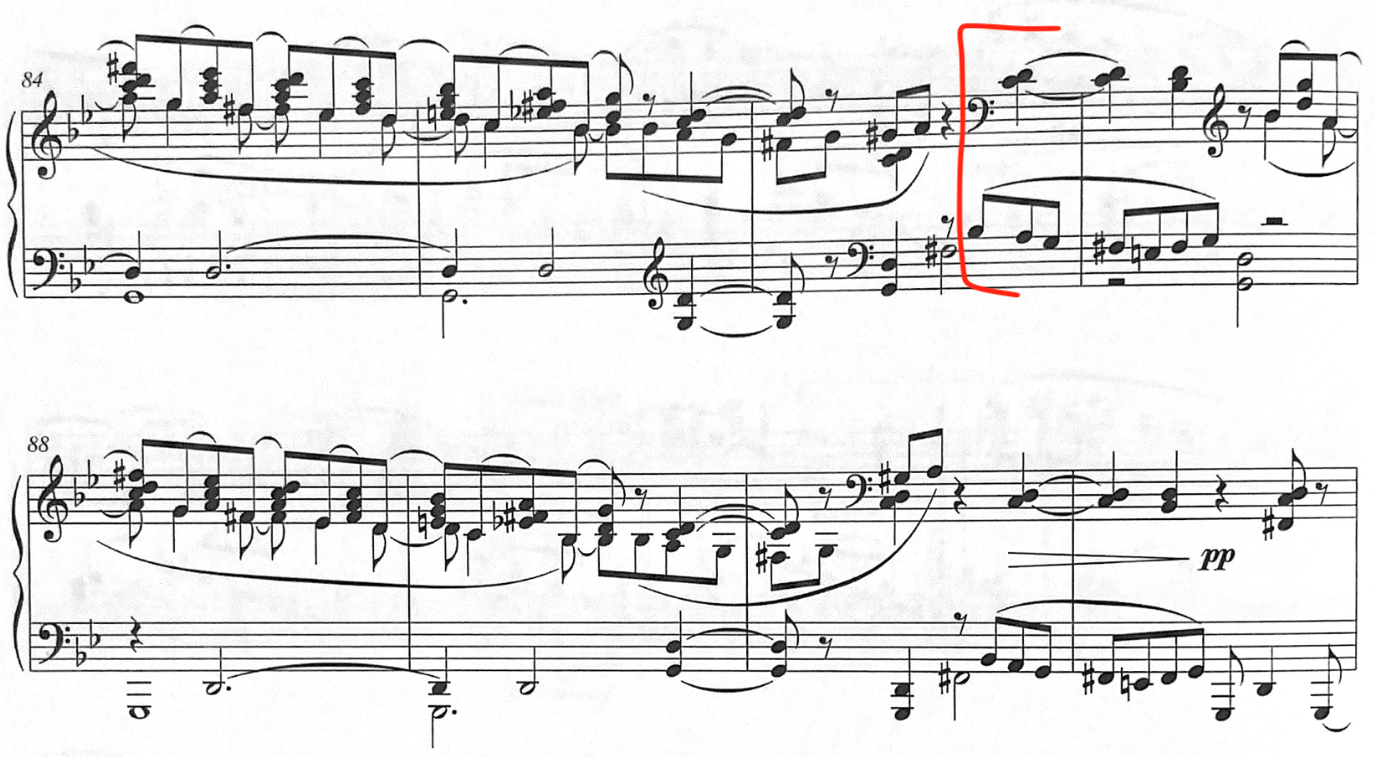
\includegraphics[width=0.8\textwidth]{t-a-prime-end-1.jpg}
  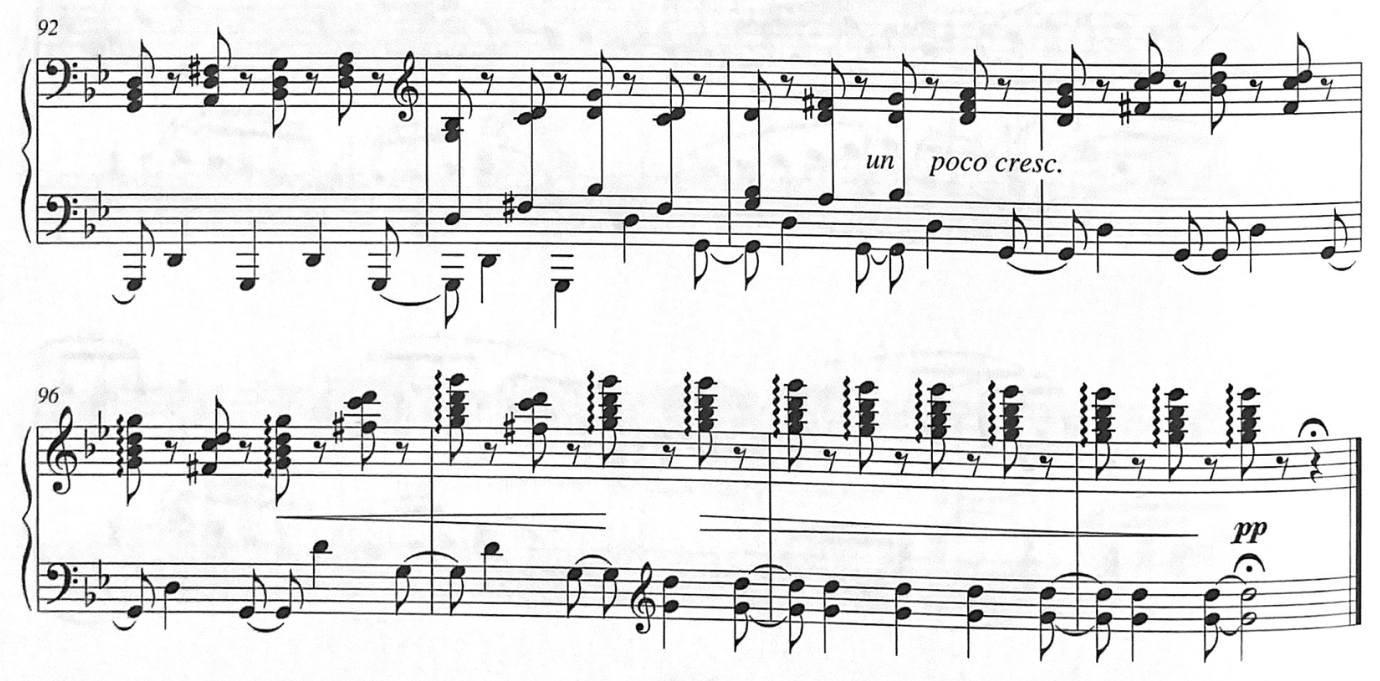
\includegraphics[width=0.8\textwidth]{t-a-prime-end-2.jpg}
  \caption{Pyotr Ilyich Tchaikovsky, The Seasons, \textit{June: Barcarolle}, mm. 84-99}
  \label{fig:t-a-prime-ending}
\end{figure}

\section{Just Around the Riverbend}

The June: Barcarolle is a character piece, meant to emulate the experience of being on a gondola ride through the canals of Venice, while a gondolier sings a folk-song. Within the first five bars of the piece, of Figure \ref{fig:t-first-three-lines}\autocite{Henle_2002}, the left-hand's motion is similar to that of a rocking boat. Measures one and two feature a rhythmic pattern of two quarter notes and a half note, with the second quarter note slurred into the half note. Then, measures three and four change and become a rhythm of four quarter notes, with the last quarter note of the measure slurred into the first quarter note of the next measure. On the fourth beat of measure 4, the last quarter note of the left-hand is slurred into the first eighth note of measure five, which begins the rockier motion of the canal's water.

It is through this emulation of the gondolier's strokes that the listener is transported themselves to the gondola ride hosted by the gondolier. As the right-hand melody enters on beat 3 of measure 2, and the Venetian gondolier begins to sing, there is a notable slow and unnerving quality to the gondolier's song. The gondolier introduces a gloomy, almost spooky atmosphere to the piece, which I aim to replicate during the A and A' sections. Though the tonic key of the piece is G Minor, as seen by G and D being the beginning two notes, Tchaikovsky employs the use of the raised seventh scale degree F\musSharp{}. Through the A and A' sections, I use this raised scale degree seven to emphasize the nature of the gondolier singing, without placing emphasis on the note itself. The note F\musSharp{} appears frequently through the two sections. Along with it, I also use a large range of dynamic contrast when additional melodic material is introduced on beat 4 of measure 12. The dynamic contrast changes from being \textit{piano} (with some crescendos and decrescendos) to being marked \textit{forte}, as in Figure \ref{fig:t-a-section-style-choices}\autocite{Henle_2002}. It is from here in measure 12 that I begin playing with a clear contrast in dynamics, and introduce a slight difference in tone as well. Prior to measure 12, my playing involves a warm feeling, relying on the notes around Middle C and below to bring about a feeling of uncertainty and spookiness. However, once I get to beat 4 of measure 12, and notes above a $C_4$ become more common, I lose the warm tone in favor of a sound that is brighter, and more closely follow the dynamic markings. In Figure \ref{fig:t-a-section-style-choices}\autocite{Henle_2002} as the note G begins the melody line, and the line rises, there is a marked \textit{forte}, along with several long crescendos and decrescendos. As I play with a bright, but also still slightly warm sound, the gondolier's song begins to sound akin to a tangent within a story. The first eleven measures of the piece are consistent in character, with a warm sound, played \textit{piano}, as the gondolier floats the listener down the canals of Venice. Then, in measures 12-22, the sound changes. It sounds as if the gondolier becomes lost in the story that they are telling, and has a sudden remembrance of a lost memory, which brought them happiness in the past, thus having a brighter tone in the song. This temporary happiness at a forgotten memory becomes dull once again in measure twenty-two, as if the gondolier remembers themself, and returns to the dramatic, and gloomy atmosphere of the song they intended to sing.

The B section of this piece begins in measure thirty-two, as in Figure \ref{fig:t-b-section-bars-32-35}\autocite{Henle_2002}. The character of this section is like that of the bright sound seen in the middle of the A section, except this section serves a different purpose. Rather than a lost memory, the B section is the climax of the story of the song the gondolier sings. There is more action, as both hands are now playing a mixture of moving quarter notes and eighth notes, rather than only the melodic line containing moving eighth notes (Figure \ref{fig:t-b-section-bars-32-35}\autocite{Henle_2002}. I also portray this faster motion, with the \textit{piano ma poco a poco crescendo} (``piano, but little by little crescendo'') and groups of four quarter notes in the melody line that are grouped together. Both of these ornamental aspects (the group of four quarter notes, and the dynamic marking to slowly increasing the dynamic volume of the section) are necessary, as I emulate the excitement of the gondolier's song. Towards the end of the B section, the gondolier sings with more syncopation to their rhythm (as in Figure \ref{fig:t-b-section-bars-44-51}\autocite{Henle_2002}). Like in the second beat of measure 45, a rhythmic pattern of dotted quarter notes slurred into an eighth note emerges. This emulates the absolute climax of the song's story. After the phrase which includes several sets of dotted quarter notes slurred into eighth notes, this is the ending of the B section. This ending involves two measures of rolled eighth notes, emphasizing the height of the song's drama the gondolier sings about. With the prolonged quarter rest which ends the B section, I play the short, one-measure long transition to the A' section as contemplative, as the protagonist of the gondolier's story returns back to thematic material of the A section, but this time as the resolution of the story.

This one-bar transition section is notable as a stark contrast to how the B section ended. While I played the rolled eighth notes of the B section quickly getting increasingly louder, while also slowing slightly with the \textit{poco ritardando}, culminating into a rolled quarter note. The transition section is a slurred three-note long eighth note, two accented quarter notes, and a held half note in the left-hand. The right-hand rests, but then in measure 53 (in Figure \ref{fig:t-a-prime-ending}\autocite{Henle_2002}), it enters very dramatically, with a tied quarter note into an eighth note. This is the entrance that I increase the dramatic nature of, as it is an entrance played \textit{mezzo forte}, and the next phrase needs to be played \textit{piano}.

Then, as the A' section ends, in beat 4 of measure 86, there is another change in thematic material. In bars 92 through to the end of the piece, as in Figure \ref{fig:t-a-prime-ending}\autocite{Henle_2002}, the left-hand's harmony becomes more dichotomous in nature. Quarter notes and eighth notes begin to alternate, in a slightly syncopated pattern. As this is no longer emulating the rocking motion of the gondola as the melody was in the A section, and the beginning of the A' section, the listener is approaching the end of the gondola ride. The motions become rockier as the listener disembarks from the gondola, and the gondolier finishes singing their song, with the melody rising in pitch to match a dramatic ending. I play this section to indicate the ending of the boat ride, to imply unsteadiness. The harmony line is no longer smooth nor reliable, instead turning to be syncopated in rhythm, and the melody line matches this. This unsteadiness is due both to the listener's physical leave of the gondola, as well as the protagonist in the gondolier's story becoming crazed. Drawn out dynamic changes, and the melody and harmony line alternating in sounding both contribute to this feeling, which I emphasize. I follow the steady increase in dynamic volume, creating a full sound in the last three measures of the piece, as the rolled quarter notes in the right-hand and un-rolled quarter notes in the left-hand take turns in sounding. I end the piece with a dramatic ending, suitable for the gondolier ending their song, with the right-hand's melody sounding quiet yet full, and the left-hand's harmony extending a tied eighth note and half note. There is a sense of unfinished business, as seen by the extended quarter note which technically ends the piece. 

\chapter[Bartók's \textit{Romanian Folk Dances}, Sz. 56, BB 68]{Béla Bartók - \textit{Romanian Folk Dances}, Sz. 56, BB 68 (1915)}

Béla Bartók (1881-1945) was a Hungarian ethnomusicologist\footnote{This involves the study of music of world culture, both of the past and present, with an emphasis on the cultural, racial, and other influences, and affects on the music.}, pianist, and composer. Bartók was born in the Austro-Hungarian Empire, in a small Hungarian city in what is present-day Romania. With parents who were teachers and amateur musicians, Bartók went on to study music at the Hungarian Royal Conservatory of Music \autocite{Burkholder_Grout_Palisca_2014}. He returned to the Conservatory in 1907 to teach, but withdrew from public musical life in 1912\autocite{Gillies}. As a teacher, Bartók did not create a distinctive ``school'' for his students, as other teachers had, disinterested in teaching piano technique or other methods. In that time, Bartók only contributed and co-authored almost 50 piano pieces (Zongoriaskola, ``Piano Method'') in 1913, for piano technique at the school\autocite{Gillies}. These pieces began his ethnomusicological studies which would become his primary method of professional musical progress and income over the next several years. Later, Bartók began searching for innately Hungarian music, leading him to collect and study peasant music from many places. Bartók would go on to publish many songs and dances, with roots in Hungary, Romania, Slovakia, Croatia, Serbia, and Bulgaria, from his travels through central Europe, Turkey, and North Africa \autocite{Burkholder_Grout_Palisca_2014}. Within the new field of ethnomusicology, Bartók edited various collections and wrote books and articles which would establish him as a leading scholar in the field. To him, Hungarian peasant music represented the music of the country better than other types of music to come out of Hungary. This view was radical for a short time, as Hungary was ruled by an urban, German-speaking elite class, but eventually prevailed \autocite{Burkholder_Grout_Palisca_2014}. Based on peasant songs and dances, he created pieces, imitating the melodies, rhythms, and other characteristics found, blending them with more classical elements from his time at studying classical music. 

Around 1908, Bartók achieved a distinctive personal style, as his compositions introduced a new aspect to the piano. It was treated as a percussive instrument rather than a melodic one \autocite{Burkholder_Grout_Palisca_2014}. When World War I (WWI) began in 1914, Bartók's travels to collect folk music became near impossible \autocite{Gillies}. Instead, Bartók turned to arranging and creating folk-based music. In 1915, the Román nepi táncok (``Romanian Folk Dances'', BB 68) was composed, and in 1918, two Hungarian piano sets--Tizenöt magyar parasztdal (``15 Hungarian Peasant Songs'', BB 79), and ``Three Hungarian Folk Tunes'', BB80b--were finished \autocite{Gillies}. In the decade after WWI, Bartók pushed towards the previously-defined limits of musical dissonance and tonal ambiguity. In his synthesis of peasant folk music with classical music, there became an emphasis on the characteristics the two styles shared, and the distinctions each had. In both peasant folk songs and classical music, pieces will typically have a tonal pitch center, and will use diatonic and other scales, with melodies built from repeated motives \autocite{Burkholder_Grout_Palisca_2014}. From the classical side, Bartók pulled on contrapuntal and formal structures and procedures, with the fugue and sonata as examples. Then, from the folk songs, he pulled the irregular meters and complex rhythms, mixed modes and modal scales, and the defining melodic structure and specific ornamentation to folk songs \autocite{Burkholder_Grout_Palisca_2014}. Music by Bartók thus became simultaneously complex in counterpoint--more than Bach's-- and rhythmically complex with more ornamentation than the folk songs he referenced. The dissonance and harmonic strategies used were also based on the mixed concepts from the two musical styles. For example, Bartók frequently uses second and fourth chords.\footnote{In a triadic chord, these chords would include the tonic, second, and fifth, and then the tonic, fourth, and fifth notes of the chord, respectively.} Aesthetically, from a classical music perspective, Bartók placed himself somewhere in between Beethoven (in terms of artistic and harmony style), and Bach (in counterpoint). Later, in 1926, the styles of Schoenberg--expressionism\footnote{A trend which is common in the twentieth-century, in which composers attempt to convey emotional value and meaning through music, above all else. Musically, expressionism will often include a higher level of dissonance than non-expressionist music, extreme dynamic contrast, angular melodies with large leaps, more to bring the intended emotion across to the listener.}-and Stravinsky--neoclassicism\footnote{A trend also commonly found in the twentieth-century, in which composers sought to return to the ``golden age'' or so of Classical-era music. This return would be to the aesthetic characteristic associated with the Classical era, including balance, clarity, and emotional restraint.}--were also emulated \autocite{Gillies}.

\section{Romanian Folk Dances, Sz. 56, BB 68}

This mixture between elements of peasant folk dances from Romania, Hungary, Bulgaria, and other countries, and traditional classical music is clear in Bartók's ``Romanian Folk Dances''. The original name for ``Romanian Folk Dances'' included the phrase ``From Hungary'' at the end, as the pieces are based on folk songs Bartók heard during his time traveling to Transylvania \autocite{Burkholder_Grout_Palisca_2014}. The title was later changed when Transylvania became part of Romania in 1920, dropping the ending ``From Hungary''. Each piece here will be referred to its most well-known title (in Romanian), with the English translation in parentheses.

\subsection{Jocul cu bâtă (``Stick Dance'')}

This piece, titled ``Jocul cu bâtă'' or ``Stick Dance'' in English, is a stick dance meant to be energetic and upbeat. As the longest piece of the six in this set, this dance was performed by men solo, as a solo dance which consists of kicking the ceiling of the room in which the dance takes place \autocite{Weissmann_1969}. These details of the dance are clearly seen in the melody. In of itself, the melody, as in  in Figure \ref{fig:bartok-stick-dance-first-line}\autocite{Lung_2016}, is not as danceable as the title suggests. Instead, the melody is more elegant in sound, with the rhythm not lending itself easily to a dance-like sound. In the first line of the dance in Figure \ref{fig:bartok-stick-dance-first-line}\autocite{Lung_2016} the rhythm of the right-hand stutters in a syncopated melody. These articulations to the melody convey to the listener that this piece is a specific type of dance not commonly found, and to the performer the specific stylistic traits found within a stick dance. In the score, as in \ref{fig:bartok-stick-dance-first-line}\autocite{Lung_2016}, Bartók marks the articulations clearly. Within the first line itself, there are dynamic markings (the \textit{forte} and crescendo denoting that the volume of the beginning starts loud, and gets louder), and phrasing markings, detailing which notes should be connected to each other. Later in the piece, there are also other markings for the stick dance's intended style: accent marks, the usage of \textit{sforzando}, \textit{tenuto} and more. Bartók carefully guided the performer to the specific idea which he wanted the music to contain, doing so by also including the specific metronome tempo marking for the quarter note (80 beats per minute would be the equivalent to one quarter note, as seen in Figure \ref{fig:bartok-stick-dance-first-line}\autocite{Lung_2016}).

\begin{figure}[h]
  \centering
  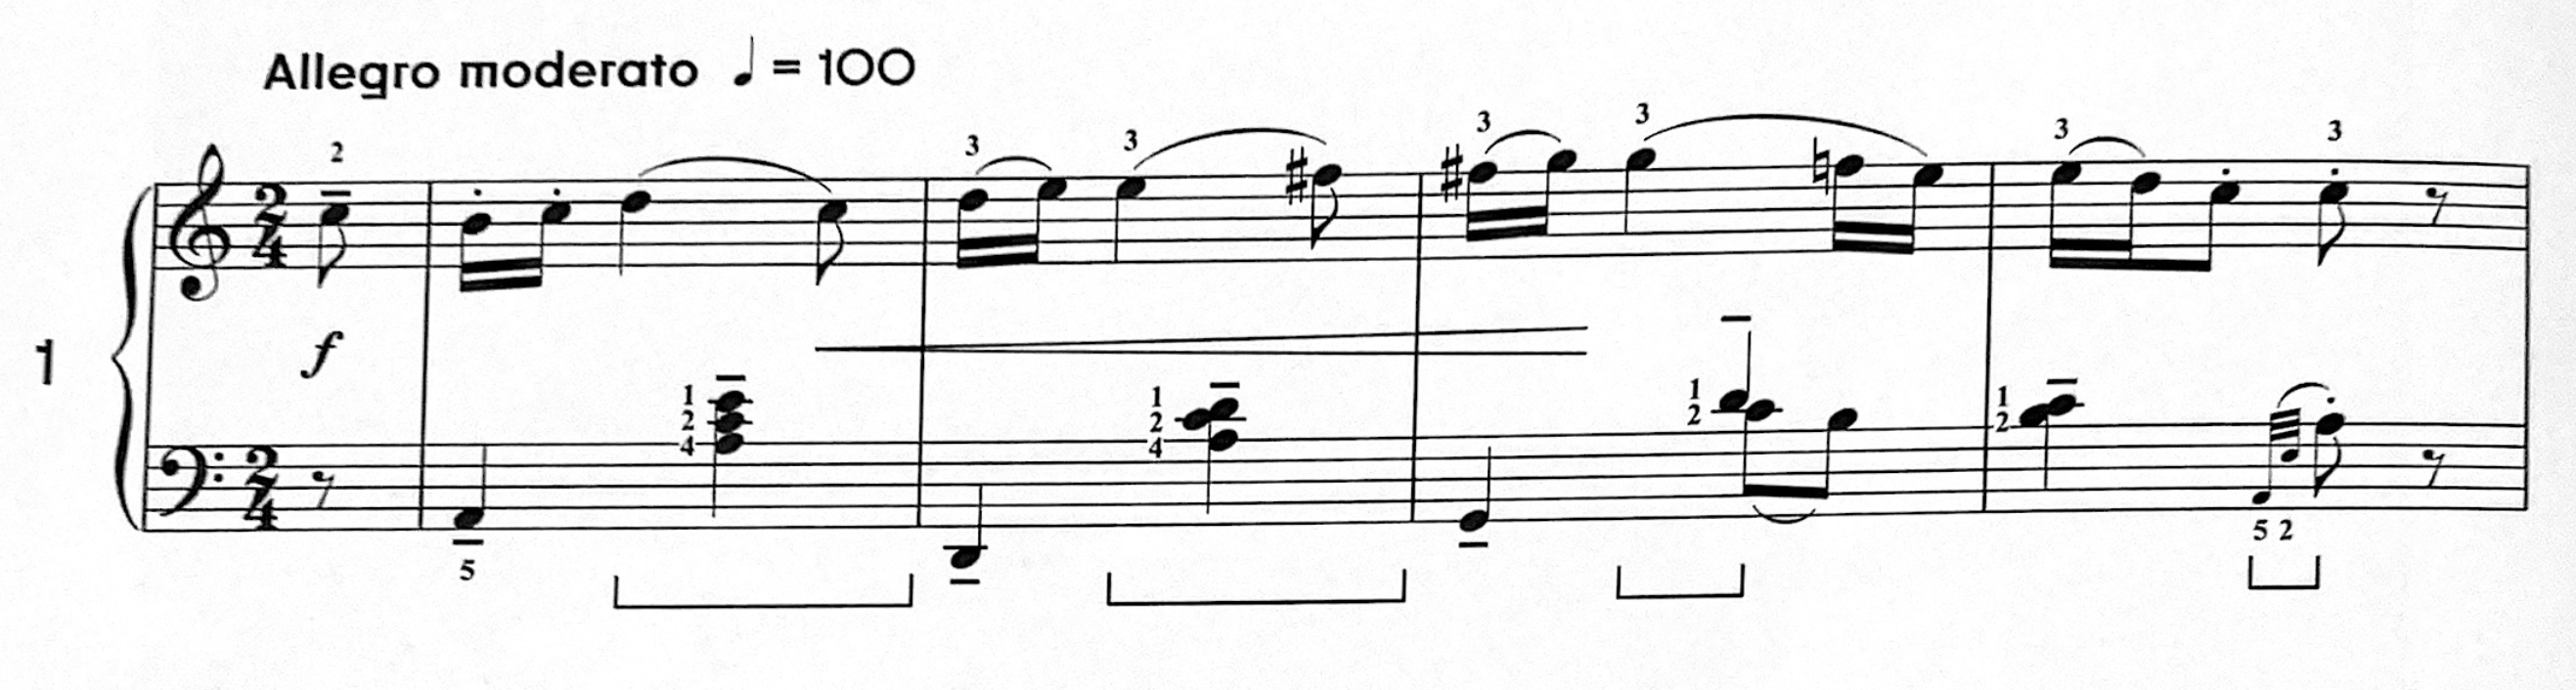
\includegraphics[width=\textwidth]{figures/bartok-stick-dance-first-line.jpg}
  \caption{Béla Bartók, Romanian Folk Dances, \textit{Jocul cu bâtă}, mm. 1-4}
  \label{fig:bartok-stick-dance-first-line}
\end{figure}


Structurally, the piece is in binary form. In the A section, which lasts from bars 1-15, the first four bars (Figure \ref{fig:bartok-stick-dance-first-line}\autocite{Lung_2016}) feature a clear suggestion Bartók wanted. In this first phrase, the first full bar features two sixteenth notes played staccato, followed by a quarter note slurred into an eighth note. This phrase has the dynamic \textit{forte}, signaling to the dancer of the piece that the music is starting, and uses the staccato of the first two notes to signify that this piece will be energetic. As opposed to the rhythms found in the B section, this section is gentler, and more dance-like, but only in comparison to the B section. 

The B section of the piece begins in measure 15. As in Figure \ref{fig:bartok-stick-dance-b-section}\autocite{Lung_2016}, the rhythm changes to include dotted rhythms, marked here in red brackets. The first full measure of this bracketed section features one set of sixteenth note triplets. These notes are meant, as Bartók notates, to sound as ornamentation and support for the dancers, instead of a rhythmic tool solely for the instrumentalist. The set of triplets is slurred with the dotted quarter note before it, and the dotted eighth and sixteenth notes after it. The dotted rhythms of the eighth and sixteen notes which appear later in the B section may imitate the sounds of the dancers hitting the ceiling with the stick.

\begin{figure}
  \centering
  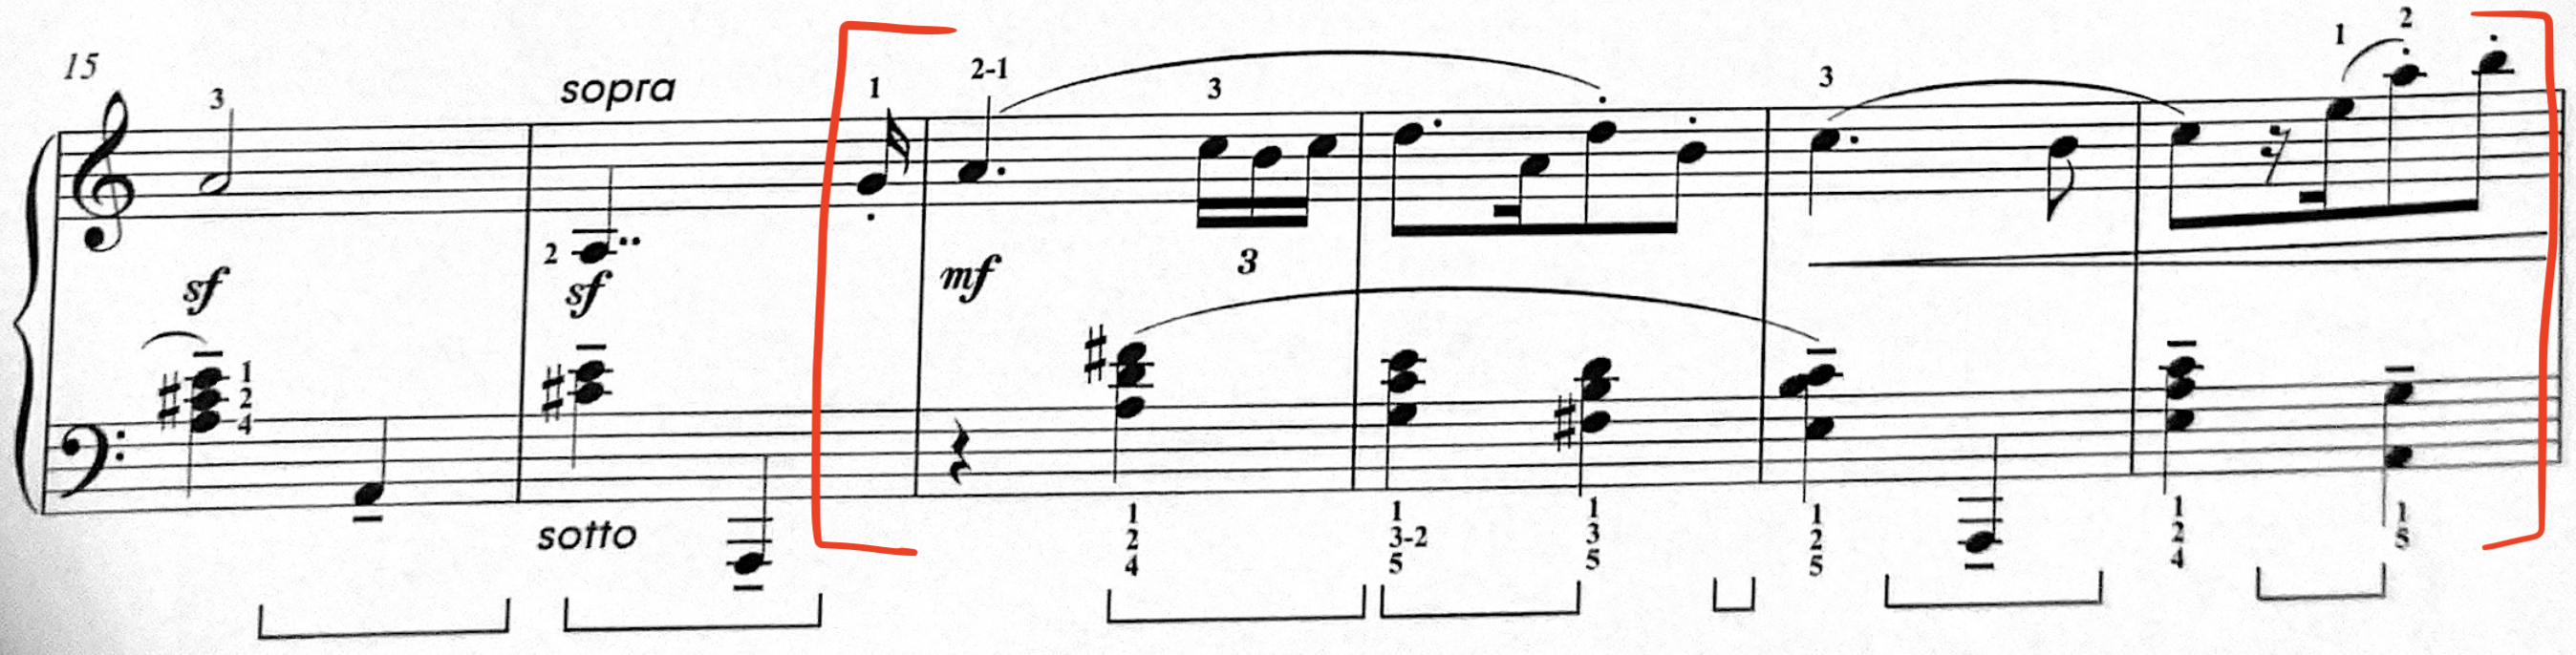
\includegraphics[width=\textwidth]{figures/bartok-stick-dance-b-section.jpg}
  \caption{Béla Bartók, Romanian Folk Dances, \textit{Jocul cu bâtă}, mm. 14-19}
  \label{fig:bartok-stick-dance-b-section}
\end{figure}

\subsubsection{Move Your Feet}

As a dance that is meant to emulate the actions of people stomping their feet while dancing and kicking the ceiling, I perform this dance with similar energy. At the beginning of the dance, as in Figure \ref{fig:bartok-stick-dance-first-line}\autocite{Lung_2016}, the left-hand's entrance is akin to the stomping of feet. It opens with a heavy rhythm of two quarter notes in the left-hand, with a \textit{tenuto}, defined as a directive in which the performer is meant to perform the indicated note or chord in a sustained manner for a longer duration than is typically assigned to the note or chords. Meanwhile, the right-hand plays an elegant melody which combined with the left-hand harmony does not lend itself easily to a dance. However, to me, as the performer, it is clear that instead of a typical danceable piece, this is a niche dance, with traits specific to the stick dance. In the first line of the dance, the dynamic level starts out \textit{forte}, and while the left-hand is played loudly, the right-hand is played even louder. This is helped by the staccato and carefully-placed legato lines in the right-hand, assisting my performance to begin the piece as loud and dramatic. In the last beat of the first full measure of Figure \ref{fig:bartok-stick-dance-first-line}\autocite{Lung_2016}, a crescendo begins, so I build even more energy into my performance. The dancers of a stick dance would not allow the climax and the height of their energy to peak at such an early point in the dance, and so neither do I in my interpretation. I still contain energy to emulate the idea of feet rapidly stomping the ground while dancing, and sticks hitting the ceiling. 

When the B section begins, this is the point in my performance where I imagine the sticks of the dance begin to hit the ceiling. As in Figure \ref{fig:bartok-stick-dance-b-section}\autocite{Lung_2016}, notes in higher octaves begin to be used more frequently. With these higher notes, I place emphasis onto passages such as measure 20, in which a sixteenth note which is slurred into an eighth note (along with the eighth note's staccato accent). Furthermore, the addition of the dotted eighth and sixteenth notes, which appear later in the B section, add to the atmosphere of sticks hitting the ceiling during the dance. I play these rhythms shorter than I play the dotted rhythms which appear elsewhere in the piece, to further emphasize the sticks hitting the ceiling, while the dancers continue at a fast pace. 

\subsection{Brâul (``Sash Dance'')}

The second of the dances in the set, Brâul (``Sash Dance''), is the shortest dance, at only two lines long. A Brâul is a typical dance out of Romania, in which traditionally a sash or other type of waistband is used as an accessory in the dance. It is a fast and energetic dance, with an undertone of sadness to the tune. This undertone is reflected in the freedom Bartók has given the performer, as in Figure \ref{fig:bartok-waistband-dance-interpretation}\autocite{Lung_2016}. The only non-rhythmic aids Bartók gives the performer is a metronome tempo marking for the quarter note, and a note to repeat the whole piece again at the end, introducing a slow \textit{ritardando} at the end. Though there is no key signature, we see that through the first bar of the piece, the left-hand signals that the tonic key of the piece will be D Minor. At the beginning of the piece, it is already energetic, with the \textit{allegro} tempo marking, and the quarter note equal to 144 beats per minute (Figure \ref{fig:bartok-waistband-dance-interpretation}\autocite{Lung_2016}). In its rhythm, each note is mostly to be played \textit{staccato}, with only a few notes played slurred, or held out with a note longer than the length of a quarter note. The melody matches this bouncy feel which the rhythm gives the piece. After each phrase, the motion of the piece as a whole stops for a moment. As in Figure \ref{fig:bartok-waistband-dance-interpretation}\autocite{Lung_2016}, there is clear, continuous motion as the melody continues on. But, as the left-hand's rhythm becomes smoother to signal a shift to a longer note, so does the melody, containing a thirty-second note before coming to a temporary close on a half-note. 

\begin{figure}[h]
  \centering
  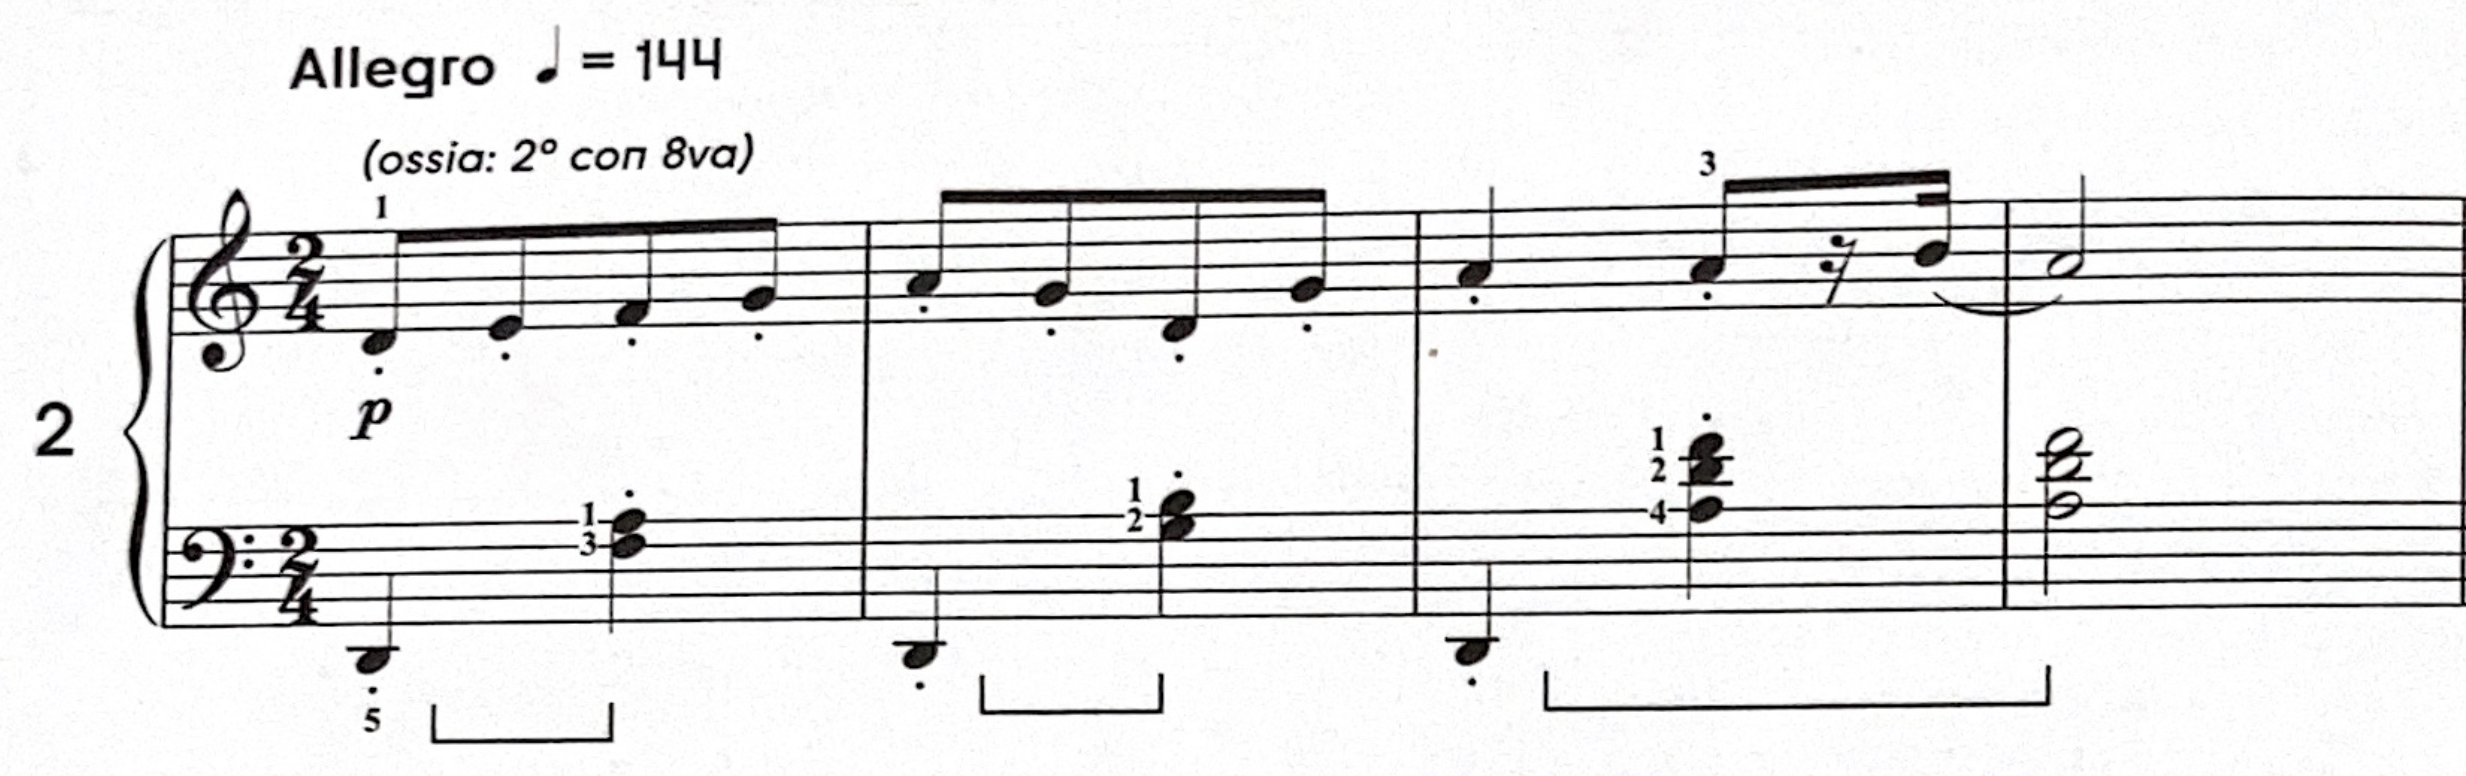
\includegraphics[width=\textwidth]{figures/bartok-waistband-dance-tempo-marking-and-dynamic.jpg}
  \caption{Béla Bartók, Romanian Folk Dances, \textit{Brâul}, mm. 1-4}
  \label{fig:bartok-waistband-dance-interpretation}
\end{figure}

\subsubsection{The Importance of a Sash}

This is the shortest dance in the six-dance set, so I do not lose the intended fast-pace energy once. This dance is flexible in rhythm, up to the performer's interpretation, as the only thing that I must keep in mind that the dance is meant to be performed \textit{allegro}, with the quarter note equal to 144 beats per minute. Knowing this, I begin the piece straightforward in rhythm, as if I were to stick to what Bartók had written exactly. The right-hand melody starts at \textit{piano}, and is staccato, while the left-hand quarter notes are both played staccato and use the pedal. But, with the dance's beginning two sounds become clear: the stomping of the feet of the dancers in the left-hand, and the sash, which is used as an accessory, in the right-hand. I also allow the left-hand's harmony to become background noise, as actually foot movements would be, had the dance taken place in-person. I emphasize the right-hand's melody, which is made easier by the staccato notes and occasional quick sixteenth note rests. For the second time playing through this piece, which is marked by the \textit{ossio: 2 con 8va} (a directive to raise the pitches played by the right-hand by an octave upon the second play through) additional energy is brought to the dance, through the raised right-hand notes. 

% dance 2
% talk about the middle section being the "sad" part of the dance, as there's that one part in the middle which is different and only slightly less upbeat, the dance itself is really start, and stop, make something up?

\subsection{Pe loc (``In One Spot'')}

The music of the second dance, ``Brâul'', flows directly into the third dance, ``Pe loc'' (``In One Spot''). It is much slower than ``Brâul'', giving a greater contrast. The beginning of the piece, as in Figure \ref{fig:bartok-one-spot-beginning}\autocite{Lung_2016}, features an overall slower melody and accompaniment. The range that the right-hand's melody plays is confined to small intervals, narrow enough to fit within the one high octave in which it is played. It is also meant to be played slowly, marked with the \textit{Andante} tempo marking, and the metronome marker of 108 beats per minute for the quarter note. The accompaniment that is found in the left-hand is that of a droning sound, as the only movement within the piece is in the melody. This gives the dance the idea that it is to be performed in one spot, as both the right-hand's melody and left-hand accompaniment stay within the range of an octave.

\begin{figure}[h]
  \centering
  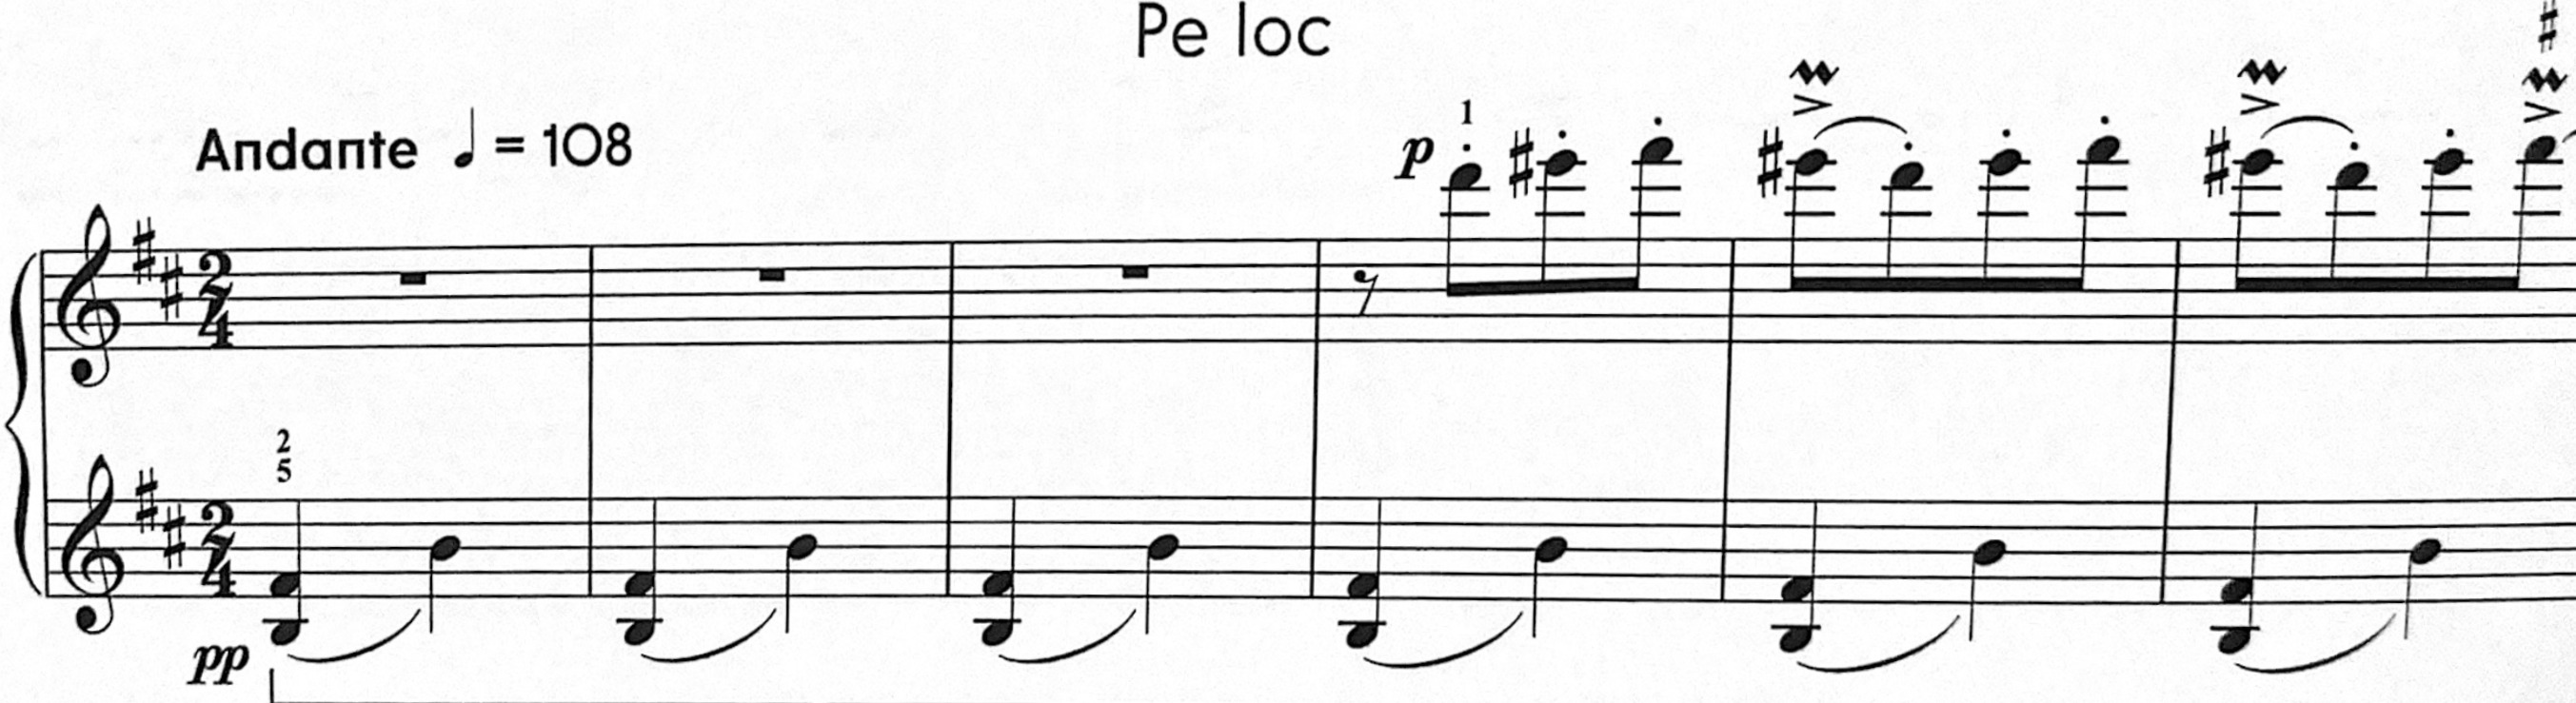
\includegraphics[width=\textwidth]{figures/bartok-one-spot-beginning.jpg}
  \caption{Béla Bartók, Romanian Folk Dances, \textit{Pe loc}, mm. 1-6}
  \label{fig:bartok-one-spot-beginning}
\end{figure}

The dance is in binary form, with sections A (measures 1-18) and B (measures 19-40). The A section starts the dance in the key of B Minor, but also features the use of the raised fourth scale degree, with the E\musSharp{} instead of E, as seen in Figure \ref{fig:bartok-one-spot-beginning}\autocite{Lung_2016}, marked in red. When E\musSharp{} is played before or after the note D, the augmented second interval is created. This augmented second interval--in which the typical one whole tone distance between one note and the next is increased by a semitone, and the resulting interval containing the distance of one and a half tones--is what creates the gypsy-like, rooted sound quality, containing the interval typical of many Middle Eastern instrumental pieces, the augmented second. The B section shifts the tonal center of the dance, modulating to D Major, the relative major key to B Minor, the tonic key found in the A section. This is found in Figure \ref{fig:bartok-one-spot-b-section}\autocite{Lung_2016}, where the left-hand accompaniment shifts to center around the chord of D Major. Similar motivic material, for both melody and harmony, is used as it was found in the A section.

\begin{figure}[h]
  \centering
  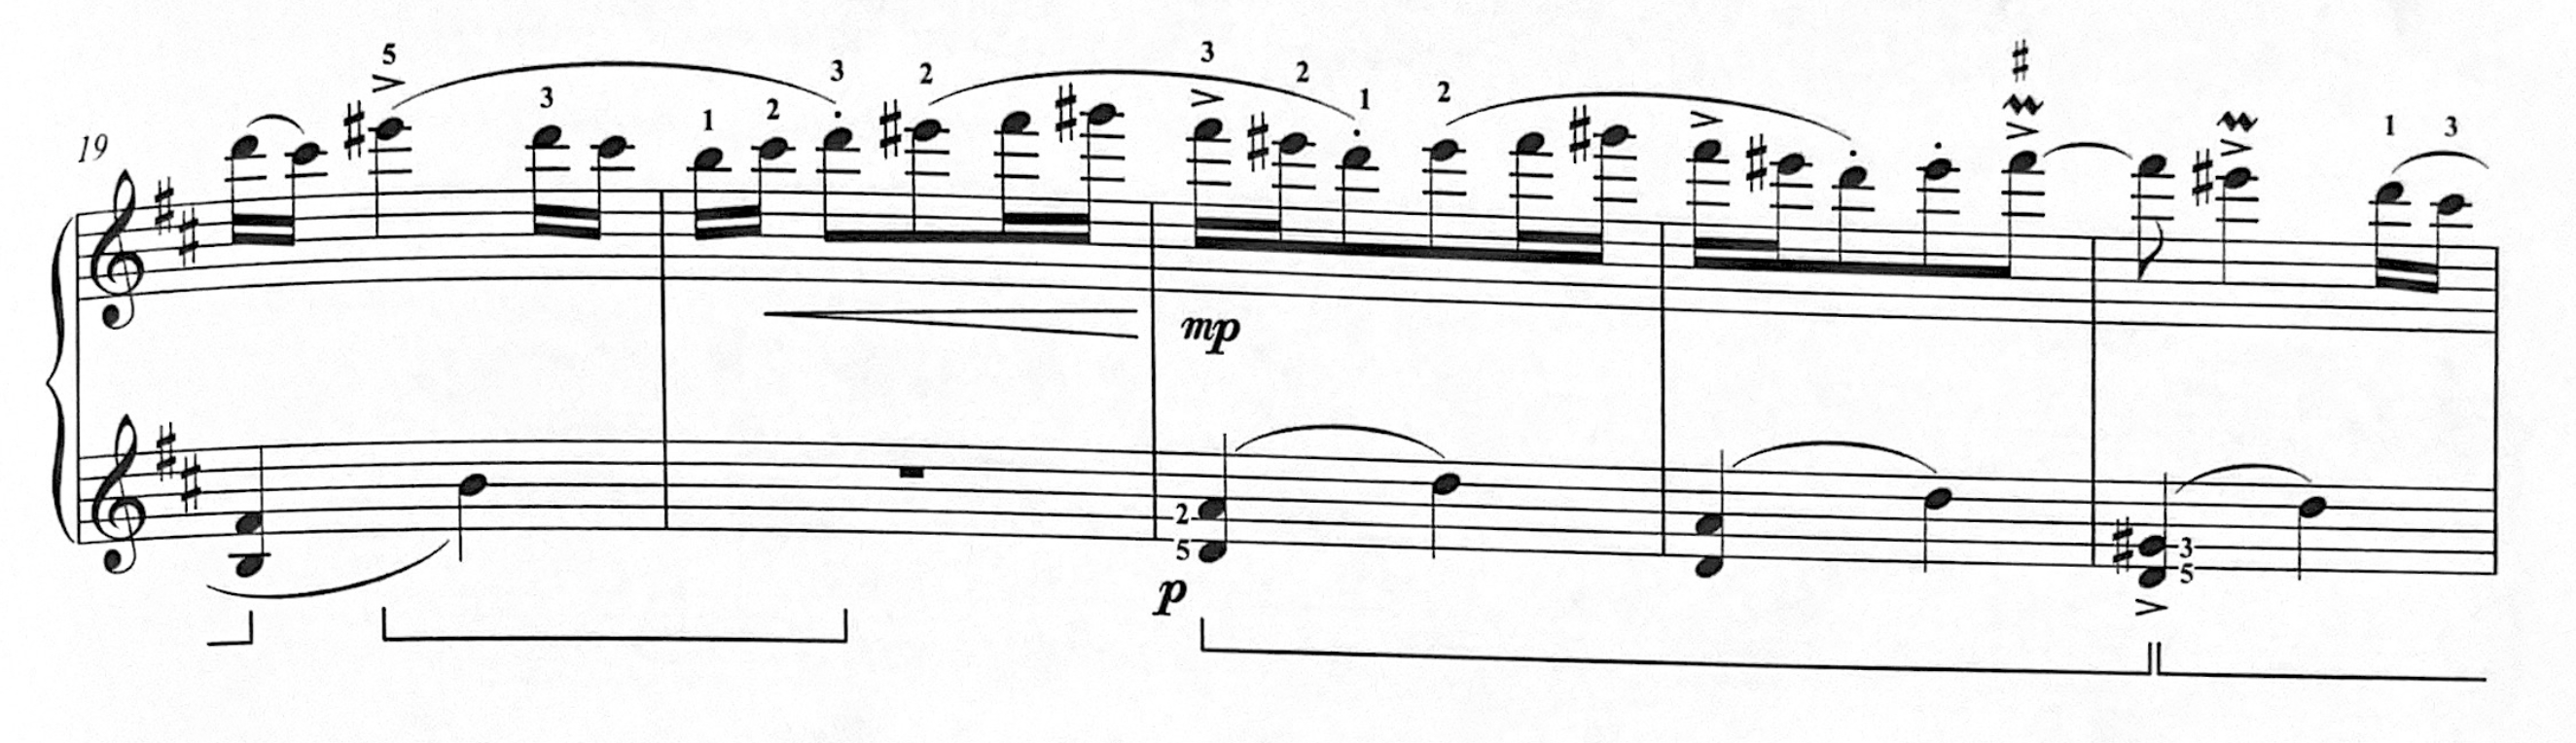
\includegraphics[width=\textwidth]{figures/bartok-one-spot-b-section.jpg}
  \caption{Béla Bartók, Romanian Folk Dances, \textit{Pe loc}, mm. 19-23}
  \label{fig:bartok-one-spot-b-section}
\end{figure}

\subsubsection{Snake Charming}

The third dance starts slow, with the \textit{Andante} tempo marking, and one quarter note equal to 108 beats per minute. To me, this indicates that this dance is meant to be mysterious in sound. Like with other dances in the set, this dance's melody is also confined to be within one octave, adding to the secretive sound. At the beginning of the dance, the left-hand is sounding quarter notes, a dyad, then a single quarter note. This becomes a droning sound that the right-hand's melody is able to to sing out above, so while the dynamic marking is \textit{piano}, I play the right-hand at a \textit{mezzo forte} level. 

It is this combination of interpretative tools, along with those previously mentioned, that causes me to correlate the sounds of a dance which is performed in a singular spot to the stereotypical ``snake charmer'' song to which United States-based audiences are familiar. This sound, known as the ``Arabian riff'' is a melody which has first been published in the nineteenth-century by Sol Bloom, a show promoter and later U.S. Congressman during the 1893 Chicago World's Colombian Exposition\autocite{Shira}. One attraction of the 1893 Exposition was called ``A Street in Cairo'' which featured snake charmers, a dancer named ``Little Egypt,'' and other Arabian and African features. The earliest known recording was created in 1895, under the name ``Streets of Cairo or The Poor Little Country Maid.'' For United States audiences especially, this melody is used to display connections to the Arabian Peninsula, which includes Iran (Persia), India, Egypt, and images of belly dancers, camels, snake charmers, or other similar ideas \autocite{Shira}.

As seen in measures 4 and 5 of James Thorton's ``Streets of Cairo or The Poor Country Maid'', in Figure \ref{fig:thorton-streets-of-cairo}\autocite{Thorton_1895} as well, the use of the major second interval is what gives this riff part of its signature sound. ``Pe loc'' does the same, as measure 4 of Figure \ref{fig:bartok-one-spot-beginning}\autocite{Lung_2016} uses the note E\musSharp{}, which is the raised scale degree two, or an augmented second interval. ``Streets of Cairo'' has the same mysterious sound quality as ``Pe loc,'' which I emulate, allowing the right-hand melody to sing above the droning of the left-hand when the pitches of the melody rise. Thus, the influences of Bartók's trips to Northern African shine through, especially in the B section of the dance, like in Figure \ref{fig:bartok-one-spot-b-section}\autocite{Lung_2016} in which sixteenth notes and eighth notes are played in some combination of legato and staccato.

\begin{figure}
  \centering
  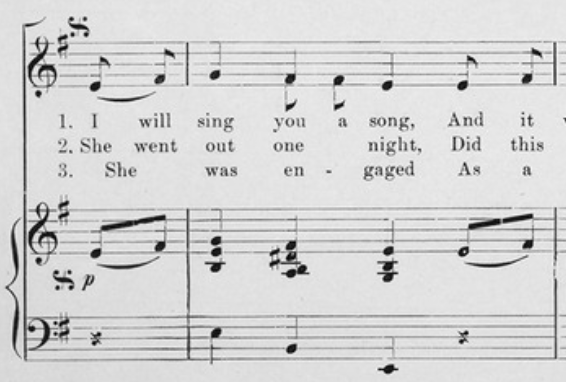
\includegraphics[width=\textwidth]{streets-of-cairo.jpg}
  \caption{James Thorton, ``Streets of Cairo or The Poor Country Maid,'' mm. 4-5}
  \label{fig:thorton-streets-of-cairo}
\end{figure}


% dance 3
% I think of a snake charmer, it's not very subtle, but it's alluring -> this is both alluding to the gypsy-like quality of the song (and as Romania was "known" to have more gypsies back then (back this point up some how), as well as the mythical quality of snake-charmers
% snake-charmer songs don't move from the one-spot, so because of Middle Eastern influences ->  The
% melody’s accents, together with the ornamentation, syncopated rhythms, and the change
% of the key center in the “B” section, are elements that could be seen in the music as a
% sound representation of the variety of visual gestures done by the dancer to make the
% dance attractive

\subsection{Buciumeana (``Dance from Bucsum'')}

The fourth dance in this set, ``Buciumeana'', comes from modern day Bucium, in Alba county in Romania. It is meant to be played slow, as evident by Figure \ref{fig:bartok-dance-four-first-line}\autocite{Lung_2016}, in which the given tempo marking is \textit{Moderato}, with quarter notes to be played at 100 beats per minute. Because it is slow, it has a childlike simplicity to it. Both rhythm and melody are simple in sound, with the left-hand accompaniment treating solely quarter notes and quarter rests. An important feature of this dance to notice, as in Figure \ref{fig:bartok-dance-four-first-line}\autocite{Lung_2016}, is that in the right-hand's melody, the shape of the melody is downwards. Every phrase in the melody goes in a downwards direction, giving the dance an almost wistful and youthful sound. This dance is constructed in binary form, with section A from measures 1-10, and section B from measures 11-18. Both sections are in the piece's tonic key of A Major, but treat slightly different thematic material. 

\begin{figure}[h]
  \centering
  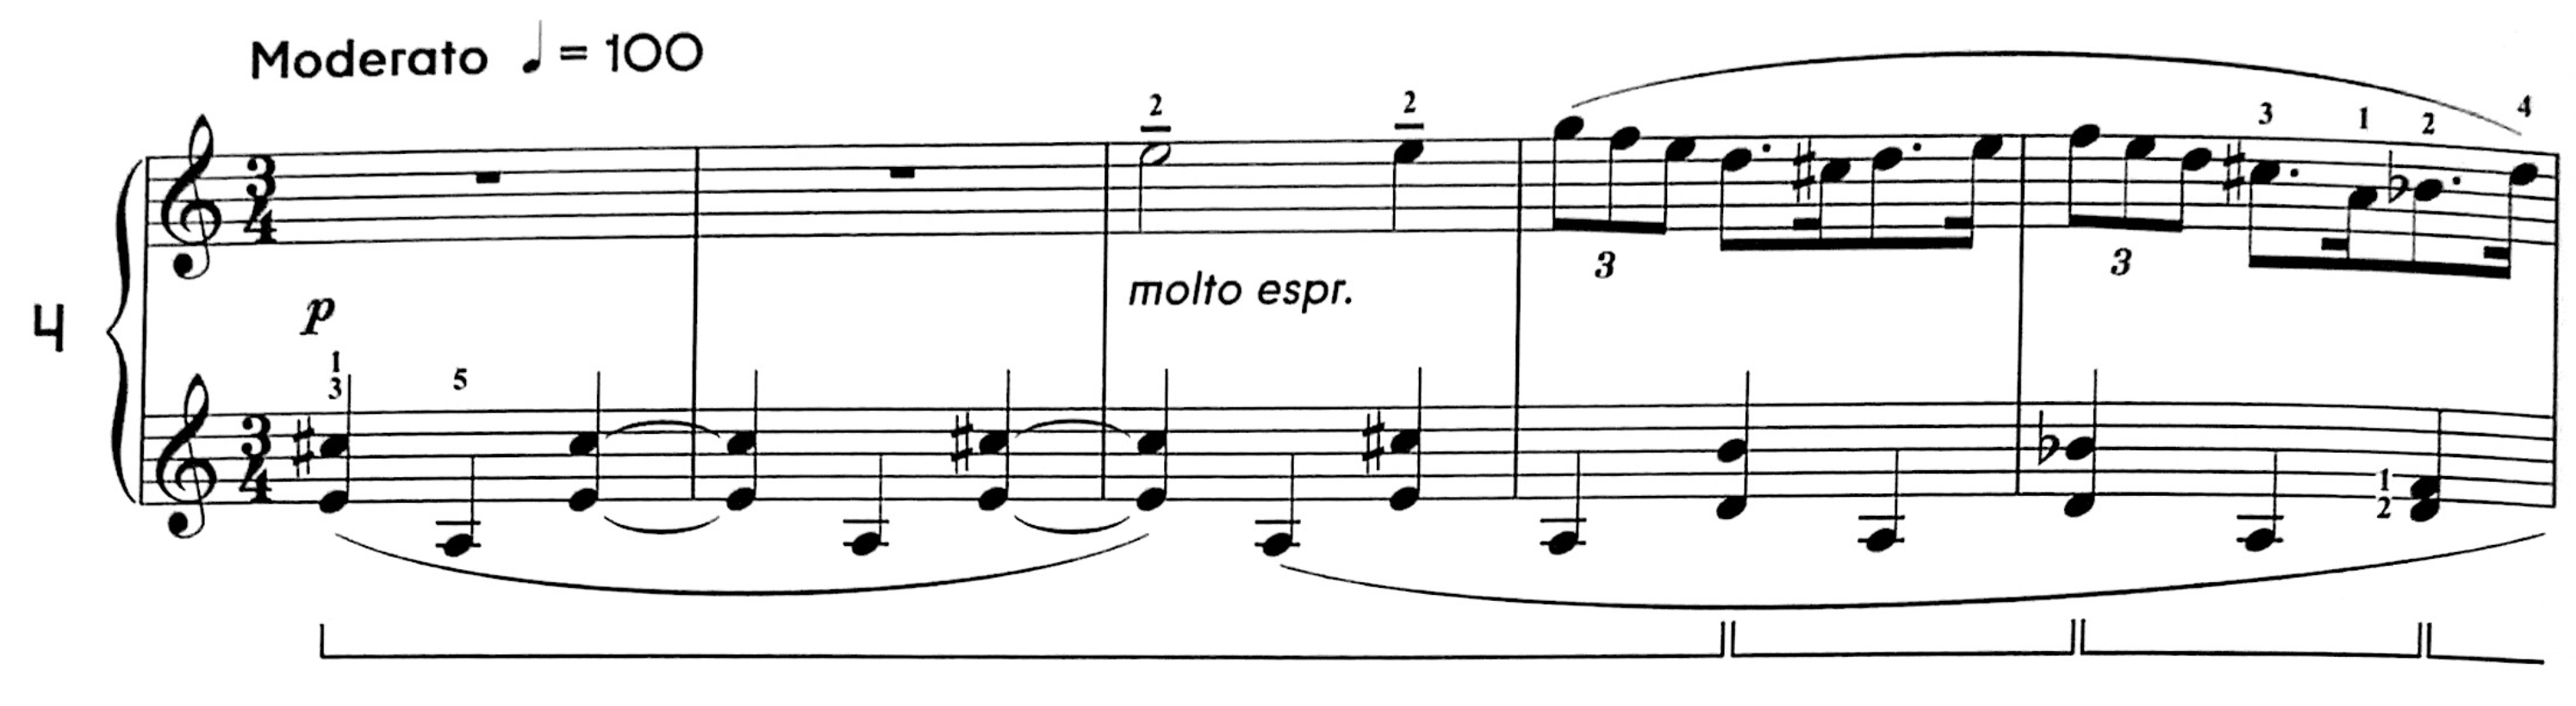
\includegraphics[width=\textwidth]{figures/bartok-dance-four-first-line.jpg}
  \caption{Béla Bartók, Romanian Folk Dances, \textit{Buciumeana}, mm. 1-5}
  \label{fig:bartok-dance-four-first-line}
\end{figure}

At the beginning of the dance, in addition to the tempo markings previously mentioned, we notice that this piece is to be played in $\frac{3}{4}$ time. This is the first dance of the set to be in $\frac{3}{4}$. However, the feeling of $\frac{3}{4}$ time is not easily felt in the first three bars of the dance. As in \ref{fig:bartok-dance-four-first-line}\autocite{Lung_2016}, the accompaniment features tied quarter notes between bars. Within the first two bars, the quarter note of the last beat of bar 1 is tied with the quarter note of the first beat of bar 2. This causes the understanding of the $\frac{3}{4}$ time signature to be unclear, until the melody enters in bar 3. Through the use of these tied notes, it will be difficult for the listener to distinguish the proper time signature of $\frac{3}{4}$ from the one they hear in the opening. The listener would hear the first two measures of the dance as being in a $\frac{2}{4}$ time signature instead, resulting in brief metric displacement for the listener. The B section of this dance introduces the beginning of sixteenth note phrases slurred together, and the feeling of more motion happening than in the A section. These long legato lines through the phrases which feature sixteenth notes in the melody and simpler quarter notes in the harmony, as seen in Figure \ref{fig:bartok-dance-four-b-section-two-lines}\autocite{Lung_2016}, convey a thoughtful sound. The long phrases with legato lines are paired with a descent in the melody. 

\begin{figure}[h]
  \centering
  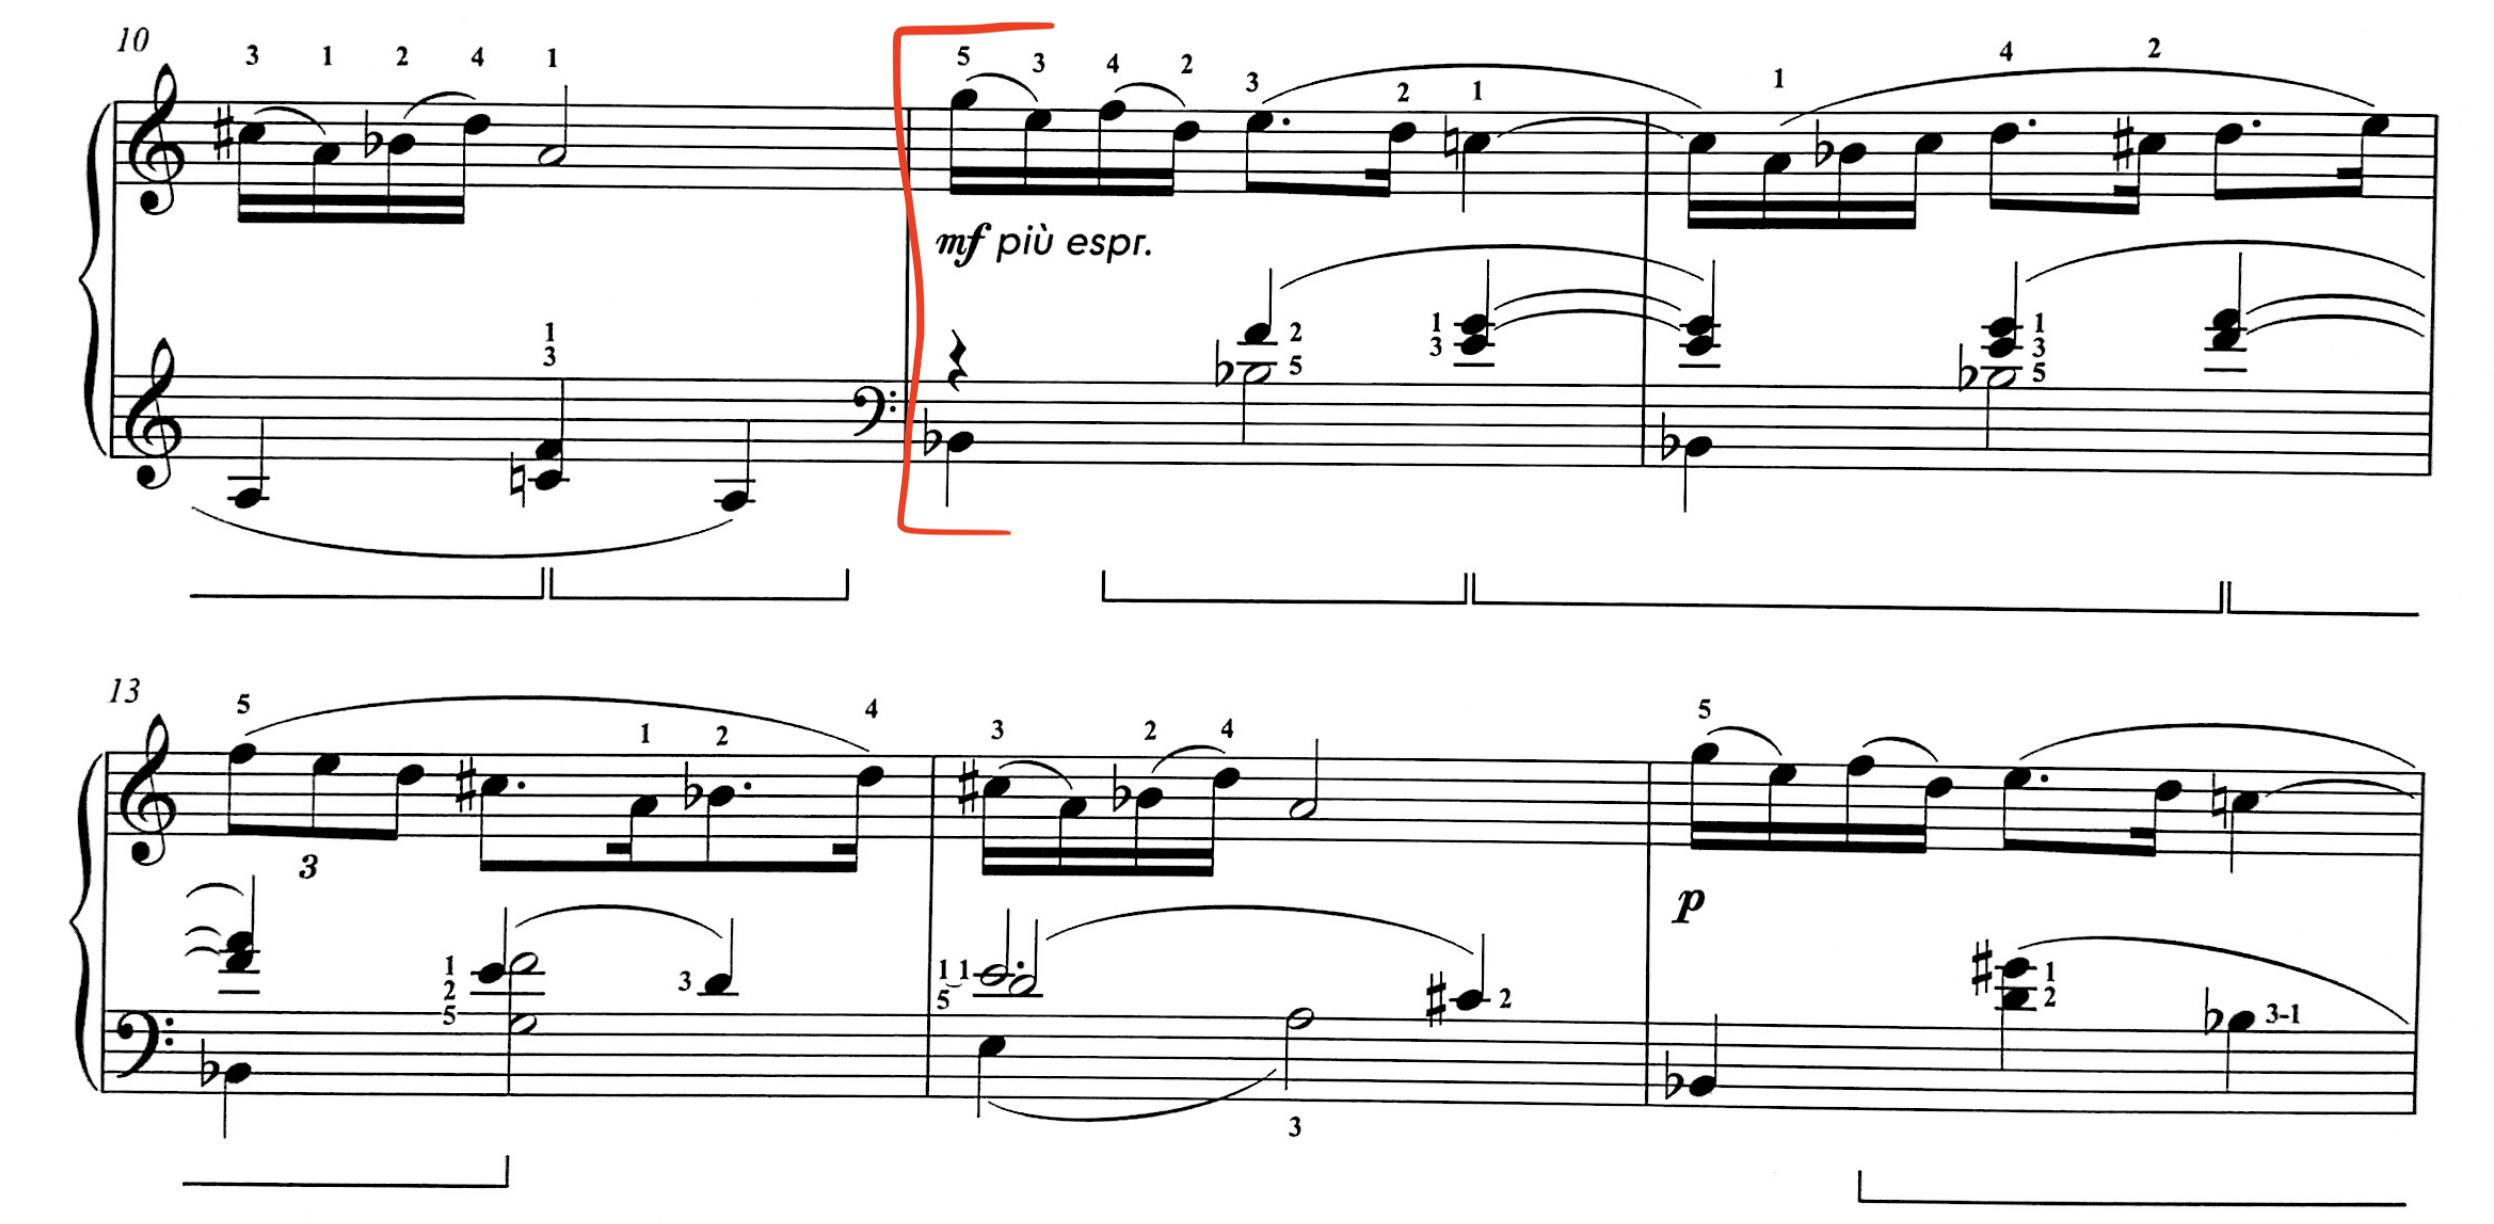
\includegraphics[width=\textwidth]{figures/bartok-dance-four-b-section-two-lines.jpg}
  \caption{Bela Bartók, Six Romanian Folk Dances, \textit{Buciumeana}, mm. 11-15}
  \label{fig:bartok-dance-four-b-section-two-lines}
\end{figure}

The similarities between sections A and B begin after the first two bars of each section. The themes in the sections become visible, as seen in figures \ref{fig:bartok-dance-four-first-line}\autocite{Lung_2016} and \ref{fig:bartok-dance-four-b-section-two-lines}\autocite{Lung_2016}. It is only the first two measures of each section which differentiates them. The first two bars of section A begin with a half note and quarter note, followed by an eighth note phrase, while the first two bars of section B begin with a phrase of sixteenth and eighth notes. After these two measures, Bartók uses the same melodic material between the two sections. 

\subsubsection{Modern Day Bucium}

The fourth dance in the six-dance set is played at a medium tempo: \textit{Moderato} in which the quarter note is to be played equivalent to 100 beats per minute. There is a childlike wonder to this dance to me, so I perform it as if it is meant to be a child dancing this piece. The first three measures of the dance, in Figure \ref{fig:bartok-dance-four-first-line}\autocite{Lung_2016}, are played with the pedal held down, and is note released until the chords played in the left-hand change. The piece begins at \textit{piano}, and the left-hand provides a simple backdrop which the right-hand is able to sing above, at a dynamic level of \textit{mezzo forte}. The phrase \textit{molto expressivo} (notated as \textit{molto espr}) also allows me to bring forth a childlike wonder to the dance. I play with the dynamic level A section; when the melody rises in pitch, I increase the dynamic level to \textit{mezzo forte}, and when the melody descends in pitch I lower the dynamic level back to \textit{piano}. Combined with motion in the right-hand, I perform the section as wistful, and a child imagining something fantastical.

The childlike wonder within the piece is more evident in the B section, when sixteenth notes are introduced in the melody line. As in Figure \ref{fig:bartok-dance-four-b-section-two-lines}\autocite{Lung_2016}, the sixteenth notes are grouped into twos, which in contrast to the quarter notes in the left-hand create a bouncy type of motion. 

% dance 4 
%The two agents are described in the first two measures of every phrase (in the “A”
%section, the order character mm. 3-4, 7-8 and in the “B” section the transgressor mm. 11-
%12, 15-16, due to the unexpected rhythmic change). The conflict between the two results
%from the rhythmic differences (see above Example 14). The order imposing character has
%triplets in its construction and dotted rhythms which makes it contrasting in itself due to
%the instability between the triplets and dotted notes. The transgressor has running
%sixteenth notes, syncopation over the bar which makes it feel weaker, and dotted rhythms.
%Even if the last phrase of the piece starts with the thematic idea of the transgressor,
%Bartók reminds the listener about the order imposing character with the last two measures
%of the phrase. This places the piece in the narrative archetype of Romance meaning that
%the order character is fulfilling its objective over the one that wanted to interfere.
%Because of this rhythmic instability between the characters, the performer has the
%opportunity to express varied nuances of yearning or longing which are characteristic to
%Romanian music. The fact that the piece ends with the same two measures that end every
%phrase up to that point it can be interpreted as recurrent obsessive statement

\subsection{``Poarga Românească'' (Romanian Polka)}

The fifth dance, ``Poarga Românească'', comes from modern day Beius, on the border between Hungary and Romania. It is reminiscent of an old Romanian dance similar to the Polka. It is notable as being the only dance in this set with a consistent alternating meter, between $\frac{3}{4}$ and $\frac{2}{4}$, in a pattern of two measures in $\frac{3}{4}$, followed by one measure in $\frac{2}{4}$, as in Figure \ref{fig:bartok-dance-five-time-signature}\autocite{Lung_2016}. This hypermeter (defined as groups of measures which form patterns of accentuation, especially at faster tempos\autocite{Hughes_Gotham_Hamm_2021}) creates a sense of asymmetry, which results in an energetic, continuous-movement in the dance, and a three-measure phrase. The last bar of this three-bar phrase is much shorter than the first two. The piece overall contains an energetic peasant-like dance theme, played in total for about a half-minute in length. The dance starts in the key of D Major, in Figure \ref{fig:bartok-dance-five-first-four-bars}\autocite{Lung_2016}, with the raised fourth scale degree G\musSharp{} (Figure \ref{fig:bartok-dance-five-time-signature}\autocite{Lung_2016}).

\begin{figure}[h]
  \centering
  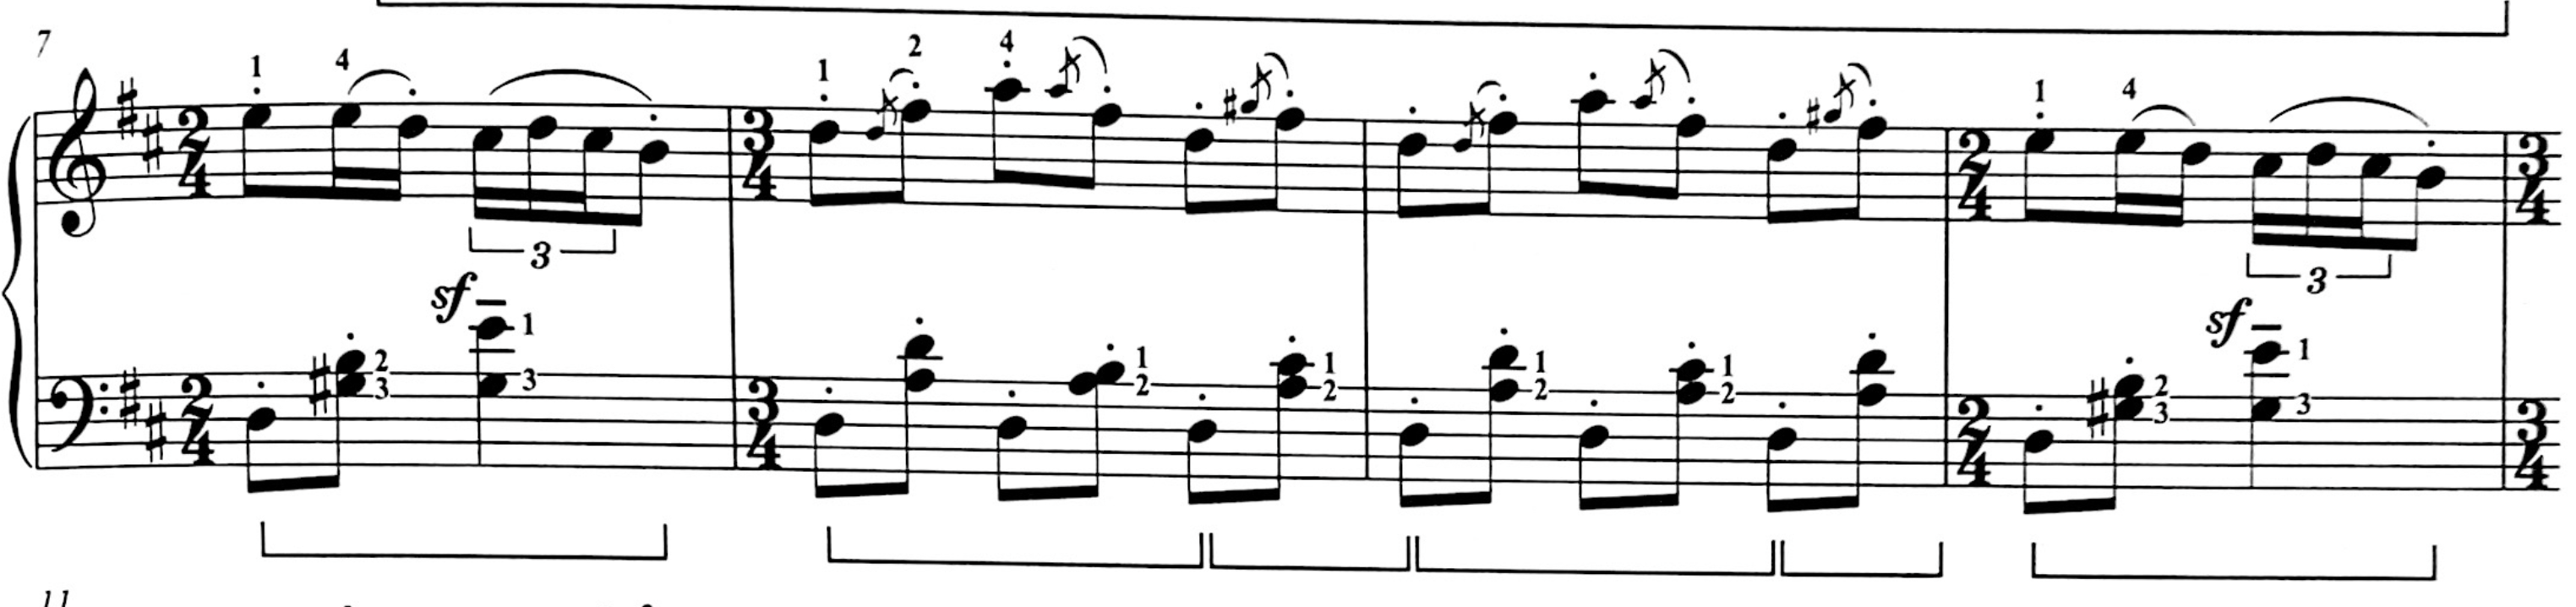
\includegraphics[width=\textwidth]{figures/bartok-dance-five-time-signature.jpg}
  \caption{Béla Bartók, Romanian Folk Dances, \textit{Poarga Românească}, mm. 7-10}
  \label{fig:bartok-dance-five-time-signature}
\end{figure}

\begin{figure}[h]
  \centering
  \includegraphics[width=\textwidth]{figures/bartok-dance-five-first-four-bars.jpg}
  \caption{Béla Bartók, Romanian Folk Dances, \textit{Poarga Românească}, mm. 1-4}
  \label{fig:bartok-dance-five-first-four-bars}
\end{figure}

Structurally, this dance is in binary form. Section A lasts from measures 1-16, and section B from measures 17-28. In the A section, the usage of \textit{staccato} and grace notes are two articulation phrases which contribute to the update, danceable nature of the piece. The \textit{staccato}, and thus the sudden bounciness of the note, adds a sense of quickness and dancing energy. The grace notes, as in Figure \ref{fig:bartok-dance-five-time-signature}\autocite{Lung_2016}, also contribute to the high-energy of the piece, with \textit{staccato} notes and slurred notes. In the B section, Bartók introduces syncopation in the left-hand's accompaniment, as in Figure \ref{fig:bartok-dance-five-b-section}\autocite{Lung_2016}. A \textit{szforzando} is added to the end of each phrase as a clear ending, such as in the last bar in Figure \ref{fig:bartok-dance-five-b-section}\autocite{Lung_2016}. Then, from bar 20 through to the end of the dance, Bartók writes a \textit{szforzando} every third measure, and in bars 25 and 28, includes a szforzando in the first and third beats of the measure (Figure \ref{fig:bartok-dance-five-b-section}\autocite{Lung_2016}), creating a contrast with the beginning of the piece. 

\begin{figure}
  \centering
  \includegraphics[width=\textwidth]{figures/bartok-dance-five-b-section.jpg}
  \caption{Béla Bartók, Romanian Folk Dances, \textit{Poarga Românească}, mm. 16-19}
  \label{fig:bartok-dance-five-b-section}
\end{figure}

\begin{figure}
  \centering
  \includegraphics[width=\textwidth]{figures/bartok-dance-five-ending.jpg}
  \caption{Béla Bartók, Romanian Folk Dances, \textit{Poarga Românească}, mm. 20-28}
  \label{fig:bartok-dance-five-ending}
\end{figure}

\subsubsection{The Polka}

Visually, the fifth of the six-dance set appear similar to a polka. To dance a polka, the dancer must be aware of the rhythm of polka. As a fast two-step, the first beat is accented, and the second beat is not. Typically, the basic step of a polka will include three steps in a quick, quick, slow rhythm, and this is the same visually as in Figure \ref{fig:bartok-dance-five-first-four-bars}\autocite{Lung_2016}, in which the first beat of measure 1 is accented by a quarter note with a tenuto mark, and beat 2 is not accented, with two eighth notes played staccato. Later, in the B section, through the rhythm of both hands, I create the perception of the strong beat landing on beat 1, and the weak beat on beat 2, of Figure \ref{fig:bartok-dance-five-b-section}\autocite{Lung_2016}. Though neither the right-hand melody nor left-hand harmony themselves contain a clear strong downbeat on beat 1, the combination does. 

\subsection{``Mărunțel`` (Fast Dance)}

\begin{figure}
  \centering
  \includegraphics[width=\textwidth]{figures/bartok-dance-six-b-section-syncopation.jpg}
  \caption{Béla Bartók, Romanian Folk Dances, \textit{Mărunțel}, mm. 20-25}
  \label{fig:bartok-dance-six-b-section-syncopation}
\end{figure}


The last dance of the set of six Romanian Folk Dances is ``Mărunțel``, which features two distinct yet similar themes. Each of these themes feels breathless in pacing, as a celebration of some kind without urgency. The beginning of the dance features a narrow melody, each of phrase of which is contained within an octave and uses small steps (Figure \ref{fig:bartok-dance-six-first-line}\autocite{Lung_2016}). As a whole, the piece is written in binary form, with section A lasting from measures 1-16, and section B from measures 17 to the end. The tonic of the piece begins in D Major, and uses a raised fourth scale degree\footnote{We should now be able to recognize the raised fourth scale degree as a feature typical of Romanian folk dances.} G\musSharp{}. At the beginning of the A section, we notice that the melodic line embodies the title of the piece (which in English translates to ``Fast Dance''), which fast melodic and harmonic phrases, as in Figure \ref{fig:bartok-dance-six-first-line}\autocite{Lung_2016}. The fast sixteenth note phrases of the section represent the fast steps dancers would need to perform to keep to the beat of the dance, but must also not be overplayed by the instrumentalist. There are also accents on also every beat to emphasize the $\frac{2}{4}$ time signature of this dance, and to provide balance against the rhythm of the harmony. When the B section begins, there is a change to the tempo, from \textit{Allegro} to the \textit{Più allegro}. There is also an introduction of triplets, which contributes to the higher-energy feeling of the B section. When the dance is played at tempo, these triplets sound as ornamentation, due to the speed at which they are played, as circled in blue in Figure \ref{fig:bartok-dance-six-b-section}\autocite{Lung_2016}. 

\begin{figure}
  \centering
  \includegraphics[width=\textwidth]{figures/bartok-dance-six-first-line.jpg}
  \caption{Béla Bartók, Romanian Folk Dances, \textit{Mărunțel}, mm. 1-6}
  \label{fig:bartok-dance-six-first-line}
\end{figure}

\begin{figure}
  \centering
  \includegraphics[width=\textwidth]{figures/bartok-dance-six-b-section.jpg}
  \caption{Béla Bartók, Romanian Folk Dances, \textit{Mărunțel}, mm. 14-19}
  \label{fig:bartok-dance-six-b-section}
\end{figure}

The B section is twice as long as the A section, with the melodic material which begins the B section returning in measure 33. However, the material does not return as an exact duplication of the first treatment of the material. There are variations to the left-hand harmony's chord progression, and Bartók eliminates the syncopated rhythm in favor of using the smoother-sounding quarter and eighth notes. By simplifying the accompaniment, the listener can focus on the melody.

\subsubsection{A Courtship}

There are two distinct themes to the last of Bartók's six dances, the ``Mărunțel.`` As a fast dance, this could be considered to be a courtship dance between two people. Each theme feels breathless in its tempo and articulation, with celebratory undertones. Within the A section, there is narrow melody, which encapsulates only one octave and no consecutive jumps larger than the interval of a third. It immediately captures the feeling the title states (``Fast Dance''), as the tempo marking for the section has one quarter note equivalent to 146 beats per minute. The person who the A section represents begins the piece fast and ready. Two accented notes, on D in the left-hand and A in the right-hand as in Figure \ref{fig:bartok-dance-six-first-line}\autocite{Lung_2016}, start the dance in \textit{forte}. The notes played staccato bring energy, while the notes that are played legato, and the pedal, do not subtract from the total energy in the piece. I mirror this, allowing the left-hand's dyads to bring the same energy as the narrow melody in the right-hand does. The power of the left-hand chords allow the right-hand's melody to stand out even more against the backdrop of motion, as the difference between the sixteenth notes and eighth notes in the right-hand and the eighth notes and quarter notes in the left-hand is clear. 

With the start of the B section, the energy and speed that was heard in the A section does not disappear; the energy of the B section includes more motion that involves syncopation and triplets. As in Figure \ref{fig:bartok-dance-six-b-section}\autocite{Lung_2016}, in the right-hand the triplets are circled in blue, which is the start of various syncopated rhythms found in the section. I try not to accent the syncopated notes themselves, but accent syncopation that falls on the strong beats of 1 and 2 in the section. Syncopation in the right-hand adds ornamentation to the piece, due to the speed at which it is played. The person represented by the B section ``dances'' twice as longe than the person who is represented by the A section (that is, the B section is twice as long as the A section), but the energy which I put into the B section does not fade. There is also a tempo change from \textit{Allegro} to \textit{Piú allegro}, in which person B is dancing faster than person A.
\chapter*{Conclusion}\label{conclusion}
\addcontentsline{toc}{chapter}{Conclusion}

\section*{Mozart and \textit{Piano Sonata in C Major No. 10}, K 330}

\section*{Beethoven and \textit{Eleven Bagatelles} Op. 119 No. 1}

\section*{Bartok and \textit{Romanian Folk Dances}, Sz. 56, BB 68}

% https://tonycalifano.blogspot.com/2008/07/bartoks-romanian-folk-dances.html

% dance 1
%left hand comes in, simulating the stomping of feet while dancing as it opens with a heavy rhythm -> talk about this foot stomping rhythm -> resulting in a dance off of two random specific individual dancers
% Because in
%the entire B section there are no rhythmic motivic elements that could remind the listener
%about the A section, the story of the piece unfolds the idea that the second character is the
%stronger one. This understanding of the work and the elements that are building it should
%give the performer a perspective on how to shape the “personalities” of the two
%characters. In other words, the AB sections can represent two dancers that compete. The
%first one is obviously overtaken by the second one which presents a more energetic,
%flamboyant and dynamic dance, characterized by dotted rhythms, more varied
%articulation, larger range of dynamics.

% dance 2
% talk about the middle section being the "sad" part of the dance, as there's that one part in the middle which is different and only slightly less upbeat, the dance itself is really start, and stop, make something up?

% dance 3
% I think of a snake charmer, it's not very subtle, but it's alluring -> this is both alluding to the gypsy-like quality of the song (and as Romania was "known" to have more gypsies back then (back this point up some how), as well as the mythical quality of snake-charmers
% snake-charmer songs don't move from the one-spot, so because of Middle Eastern influences ->  The
% melody’s accents, together with the ornamentation, syncopated rhythms, and the change
% of the key center in the “B” section, are elements that could be seen in the music as a
% sound representation of the variety of visual gestures done by the dancer to make the
% dance attractive

% dance 4 
%The two agents are described in the first two measures of every phrase (in the “A”
%section, the order character mm. 3-4, 7-8 and in the “B” section the transgressor mm. 11-
%12, 15-16, due to the unexpected rhythmic change). The conflict between the two results
%from the rhythmic differences (see above Example 14). The order imposing character has
%triplets in its construction and dotted rhythms which makes it contrasting in itself due to
%the instability between the triplets and dotted notes. The transgressor has running
%sixteenth notes, syncopation over the bar which makes it feel weaker, and dotted rhythms.
%Even if the last phrase of the piece starts with the thematic idea of the transgressor,
%Bartok reminds the listener about the order imposing character with the last two measures
%of the phrase. This places the piece in the narrative archetype of Romance meaning that
%the order character is fulfilling its objective over the one that wanted to interfere.
%Because of this rhythmic instability between the characters, the performer has the
%opportunity to express varied nuances of yearning or longing which are characteristic to
%Romanian music. The fact that the piece ends with the same two measures that end every
%phrase up to that point it can be interpreted as recurrent obsessive statement

%%%%%%%%%%%%%%%%%%%%%%%%%%%%%%%%%%%%%%%%%%%%%%%%%%%%%%%
%
%  This section starts the back matter. The back matter includes appendices, indicies, and the
%  bibliography
%
%%%%%%%%%%%%%%%%%%%%%%%%%%%%%%%%%%%%%%%%%%%%%%%%%%%%%%%

\backmatter

% %!TEX root = ../username.tex
%%%%%%%%%%%%%%%%%%%%%%%%%%%%%%%%%%%%%%%%%%%%%%%%%%%%%%%%%%%%%%%%
% Contents: Math typesetting with LaTeX
% $Id: math.tex,v 1.3 2005/05/21 02:03:43 jonb Exp $
%%%%%%%%%%%%%%%%%%%%%%%%%%%%%%%%%%%%%%%%%%%%%%%%%%%%%%%%%%%%%%%%%

\chapter{Typesetting Mathematical Formulae}\label{math}
\begin{intro}
  This appendix is taken from \citet{ophs03} under the GNU open source documentation license. This appendix addresses the main strength
  of \TeX{}: mathematical typesetting. But be warned, this appendix
  only scratches the surface. While the things explained here are
  sufficient for many people, don't despair if you can't find a
  solution to your mathematical typesetting needs here. It is highly likely
  that your problem is addressed in \AmS-\LaTeX{}%
  \footnote{\texttt{CTAN:/tex-archive/macros/latex/packages/amslatex}}
  or some other package.
\end{intro}
  
\section{General}

\LaTeX{} has a special mode for typesetting mathematics\index{mathematics}.
Mathematical text within a paragraph is entered between \verb|\(|\index{\(@\verb+\(+}
and \verb|\)|\index{\)@\verb+\)+}, %$
between \texttt{\$} and \texttt{\$} or between
\verb|\begin{|{math}\verb|}| and \verb|\end{math}|.\index{formulae}

\begin{singlespace}
\begin{example}
Add $a$ squared and $b$ squared 
to get $c$ squared. Or, using 
a more mathematical approach:
$c^{2}=a^{2}+b^{2}$
\end{example}
\end{singlespace}

\begin{singlespace}
\begin{example}
\TeX{} is pronounced as 
$\tau\epsilon$.\\[6pt]
100~m$^{3}$ of water\\[6pt]
This comes from my $\heartsuit$
\end{example}
\end{singlespace}

It is preferable to \emph{display} larger mathematical equations or formulae,
rather than to typeset them on separate lines. This means you enclose them
in \verb|\[| \index{\[@\verb+\[+} and \verb|\]| \index{\]@\verb+\]+} or between
\verb|\begin{|displaymath\index{displaymath}\verb|}| and
  \verb|\end{displaymath}|.  This produces formulae which are not
numbered. If you want \LaTeX{} to number them, you can use the
equation\index{equation} environment.


\begin{singlespace}
\begin{example}
Add $a$ squared and $b$ squared 
to get $c$ squared. Or, using 
a more mathematical approach:
\begin{displaymath}
c^{2}=a^{2}+b^{2}
\end{displaymath}
And just one more line.
\end{example}
\end{singlespace}

You can reference an equation with \ic{label} and \ic{ref}

\begin{singlespace}
\begin{example}
\begin{equation} \label{eq:eps}
\epsilon > 0
\end{equation}
From (\ref{eq:eps}), we gather 
\ldots
\end{example}
\end{singlespace}

Note that expressions will be typeset in a different style if displayed:

\begin{singlespace}
\begin{example}
$\lim_{n \to \infty} 
\sum_{k=1}^n \frac{1}{k^2} 
= \frac{\pi^2}{6}$
\end{example}
\end{singlespace}
\begin{singlespace}
\begin{example}
\begin{displaymath}
\lim_{n \to \infty} 
\sum_{k=1}^n \frac{1}{k^2} 
= \frac{\pi^2}{6}
\end{displaymath}
\end{example}
\end{singlespace}

There are differences between \emph{math mode} and \emph{text mode}. For
example in \emph{math mode}: 

\begin{enumerate}

\item Most spaces and linebreaks do not have any significance, as all spaces
either are derived logically from the mathematical expressions or
have to be specified using special commands such as \verb|\,| \index{''\,@\verb+\,+}, \ic{quad}, or \ic{qquad}.
 
\item Empty lines are not allowed. Only one paragraph per formula.

\item Each letter is considered to be the name of a variable and will be
typeset as such. If you want to typeset normal text within a formula
(normal upright font and normal spacing) then you have to enter the
text using the \verb|\textrm{...}| commands.
\end{enumerate}


\begin{singlespace}
\begin{example}
\begin{equation}
\forall x \in \mathbf{R}:
\qquad x^{2} \geq 0
\end{equation}
\end{example}
\end{singlespace}

\begin{singlespace}
\begin{example}
\begin{equation}
x^{2} \geq 0\qquad
\textrm{for all }x\in\mathbf{R}
\end{equation}
\end{example}
\end{singlespace}

Mathematicians can be very fussy about which symbols are used:
it would be conventional here to use `blackboard bold\index{blackboard bold}',
bold symbols\index{bold symbols} which is obtained using \ic{mathbb} from the
package \ip{amsfonts} or \ip{amssymb}.

\ifx\mathbb\undefined\else
The last example becomes
\begin{singlespace}
\begin{example}
\begin{displaymath}
x^{2} \geq 0\qquad
\textrm{for all }x\in\mathbb{R}
\end{displaymath}
\end{example}
\end{singlespace}
\fi

\section{Grouping in Math Mode}

Most math mode commands act only on the next character. So if you
want a command to affect several characters, you have to group them
together using curly braces: \verb|{...}|.

\begin{singlespace}
\begin{example}
\begin{equation}
a^x+y \neq a^{x+y}
\end{equation}
\end{example}
\end{singlespace}
 
\section{Building Blocks of a Mathematical Formula}

In this section, the most important commands used in mathematical
typesetting will be described. Take a look at \citet{kd03} for a detailed list of commands for typesetting
mathematical symbols.

\textbf{Lowercase Greek letters\index{Greek letters}} are entered as \verb|\alpha|,
 \verb|\beta|, \verb|\gamma|, \ldots, uppercase letters
are entered as \verb|\Gamma|, \verb|\Delta|, \ldots\footnote{There is no
  uppercase Alpha defined in \LaTeXe{} because it looks the same as a
  normal roman A. Once the new math coding is done, things will
  change.} 

\begin{singlespace}
\begin{example}
$\lambda,\xi,\pi,\mu,\Phi,\Omega$
\end{example}
\end{singlespace}
 
\textbf{Exponents and Subscripts} can be specified using\index{exponent}\index{subscript}
the \verb|^|\index{^@\verb+^+} and the \verb|_|\index{_@\verb+_+} character.

\begin{singlespace}
\begin{example}
$a_{1}$ \qquad $x^{2}$ \qquad
$e^{-\alpha t}$ \qquad
$a^{3}_{ij}$\\
$e^{x^2} \neq {e^x}^2$
\end{example}
\end{singlespace}

The \textbf{square root\index{square root}} is entered as \ic{sqrt}, the
$n^\mathrm{th}$ root is generated with \verb|\sqrt[|$n$\verb|]|. The size of
the root sign is determined automatically by \LaTeX. If just the sign
is needed, use \ic{surd}.

\begin{singlespace}
\begin{example}
$\sqrt{x}$ \qquad 
$\sqrt{ x^{2}+\sqrt{y} }$ 
\qquad $\sqrt[3]{2}$\\[3pt]
$\surd[x^2 + y^2]$
\end{example}
\end{singlespace}

The commands \ic{overline} and \ic{underline} create
\textbf{horizontal lines} directly over or under an expression.
\index{horizontal!line}

\begin{singlespace}
\begin{example}
$\overline{m+n}$
\end{example}
\end{singlespace}

The commands \ic{overbrace} and \ic{underbrace} create
long \textbf{horizontal braces} over or under an expression.
\index{horizontal!brace}

\begin{singlespace}
\begin{example}
$\underbrace{ a+b+\cdots+z }_{26}$
\end{example}
\end{singlespace}

\index{mathematical!accents} To add mathematical accents such as small
arrows or {tilde} signs to variables, you can use the commands
given in \citet{kd03}.  Wide hats and
tildes covering several characters are generated with \ic{widetilde}
and \ic{widehat}.  The \verb|'|\index{'@\verb+'+} symbol gives a
prime\index{prime}.
% a dash is --

\begin{singlespace}
\begin{example}
\begin{displaymath}
y=x^{2}\qquad y'=2x\qquad y''=2
\end{displaymath}
\end{example}
\end{singlespace}

\textbf{Vectors}\index{vectors} often are specified by adding a small
arrow symbol\index{arrow symbols} on top of a variable. This is done with the
\ic{vec} command. The two commands \ic{overrightarrow} and
\ic{overleftarrow} are useful to denote the vector from $A$ to $B$.

\begin{singlespace}
\begin{example}
\begin{displaymath}
\vec a\quad\overrightarrow{AB}
\end{displaymath}
\end{example}
\end{singlespace}

Names of log-like functions are often typeset in an upright
font and not in italic like variables. Therefore \LaTeX{} supplies the
following commands to typeset the most important function names:
\index{mathematical!functions}

\begin{singlespace}
\begin{verbatim}
\arccos   \cos    \csc   \exp   \ker     \limsup  \min   \sinh
\arcsin   \cosh   \deg   \gcd   \lg      \ln      \Pr    \sup
\arctan   \cot    \det   \hom   \lim     \log     \sec   \tan
\arg      \coth   \dim   \inf   \liminf  \max     \sin   \tanh
\end{verbatim}
\end{singlespace}

\begin{singlespace}
\begin{example}
\[\lim_{x \rightarrow 0}
\frac{\sin x}{x}=1\]
\end{example}
\end{singlespace}

For the modulo function\index{modulo function}, there are two commands: \ic{bmod} for the
binary operator ``$a \bmod b$'' and \ic{pmod}
for expressions
such as ``$x\equiv a \pmod{b}$.''

A built-up \textbf{fraction\index{fraction}} is typeset with the
\ic{frac}\verb|{...}{...}| command.
Often the slashed form $1/2$ is preferable, because it looks better
for small amounts of `fraction material.'

\begin{singlespace}
\begin{example}
$1\frac{1}{2}$~hours
\begin{displaymath}
\frac{ x^{2} }{ k+1 }\qquad
x^{ \frac{2}{k+1} }\qquad
x^{ 1/2 }
\end{displaymath}
\end{example}
\end{singlespace}

To typeset binomial coefficients or similar structures, you can use
either the command \linebreak \ic{binom}\{\emph{num}\}\{\emph{denom}\} or \ic{genfrac}\{\emph{ldelim}\}\{\emph{rdelim}\}\{\emph{thickness}\}\{\emph{style}\}\{\emph{num}\}\{\emph{denom}\}. The second command can be used to produce customized fraction like output and more information can be found in \citet{mgbcr04}.

\begin{singlespace}
\begin{example}
\begin{displaymath}
\binom{n}{k}\qquad 
\genfrac{}{}{0pt}{}{x}{y+2}
\end{displaymath}
\end{example}
\end{singlespace}
 
\medskip

The \textbf{integral operator\index{integral operator}} is generated with \ic{int}, the
\textbf{sum operator\index{sum operator}} with \ic{sum}. The upper and lower limits
are specified with~\verb|^|\index{^@\verb+^+} and~\verb|_|\index{_@\verb+_+} like subscripts and superscripts.

\begin{singlespace}
\begin{example}
\begin{displaymath}
\sum_{i=1}^{n} \qquad
\int_{0}^{\frac{\pi}{2}} \qquad
\end{displaymath}
\end{example}
\end{singlespace}

For \textbf{braces\index{braces}} and other delimiters\index{delimiters}, there exist all
types of symbols in \TeX{} (e.g.~$[\;\langle\;\|\;\updownarrow$).
Round and square braces can be entered with the corresponding keys,
curly braces with \verb|\{|, all other delimiters are generated with
special commands (e.g.~\verb|\updownarrow|). For a list of all
delimiters available, check \citet{kd03}.

\begin{singlespace}
\begin{example}
\begin{displaymath}
{a,b,c}\neq\{a,b,c\}
\end{displaymath}
\end{example}
\end{singlespace}

If you put the command \ic{left} in front of an opening delimiter or
\ic{right} in front of a closing delimiter, \TeX{} will automatically
determine the correct size of the delimiter. Note that you must close
every \ic{left} with a corresponding \ic{right}, and that the size is
determined correctly only if both are typeset on the same line. If you
don't want anything on the right, use the invisible `\verb|\right .|\index{commands!right@\verb+right .+}'!

\begin{singlespace}
\begin{example}
\begin{displaymath}
1 + \left( \frac{1}{ 1-x^{2} }
    \right) ^3
\end{displaymath}
\end{example}
\end{singlespace}

In some cases it is necessary to specify the correct size of a
mathematical delimiter\index{mathematical!delimiter} by hand,
which can be done using the commands \ic{big}, \ic{Big}, \ic{bigg} and
\ic{Bigg} as prefixes to most delimiter commands.\footnote{These
  commands do not work as expected if a size changing command has been
  used, or the \texttt{11pt} or \texttt{12pt} option has been
  specified.  Use the exscale\index{exscale} or amsmath\index{amsmath} packages to
  correct this behaviour.}

\begin{singlespace}
\begin{example}
$\Big( (x+1) (x-1) \Big) ^{2}$\\
$\big(\Big(\bigg(\Bigg($\quad
$\big\}\Big\}\bigg\}\Bigg\}$\quad
$\big\|\Big\|\bigg\|\Bigg\|$
\end{example}
\end{singlespace}

To enter \textbf{three dots\index{three dots}} into a formula, you can use several
commands. \ic{ldots} typesets the dots on the baseline, \ic{cdots}
sets them centered. Besides that, there are the commands \ic{vdots} for
vertical and \ic{ddots} for diagonal dots\index{diagonal dots}.\index{vertical
  dots}\index{horizontal!dots} You can find another example in section~\ref{sec:vert}.

\begin{singlespace}
\begin{example}
\begin{displaymath}
x_{1},\ldots,x_{n} \qquad
x_{1}+\cdots+x_{n}
\end{displaymath}
\end{example}
\end{singlespace}
 
\section{Math Spacing}

\index{math spacing} If the spaces within formulae chosen by \TeX{}
are not satisfactory, they can be adjusted by inserting special
spacing commands. There are some commands for small spaces: \verb|\,| \index{\,@\verb+\,+} for
$\frac{3}{18}\:\textrm{quad}$ (\demowidth{0.166em}), \verb|\:| \index{\:@\verb+\:+} for $\frac{4}{18}\:
\textrm{quad}$ (\demowidth{0.222em}) and \verb|\;| \index{\;@\verb+\;+} for $\frac{5}{18}\:
\textrm{quad}$ (\demowidth{0.277em}).  The escaped space character
\verb*.\ . generates a medium sized space and \ic{quad}
(\demowidth{1em}) and \ic{qquad} (\demowidth{2em}) produce large
spaces. The size of a quad corresponds to the width of the
character `M' of the current font.  The \verb|\!|\index{"\"!@\texttt{\bs"!}} command produces a
negative space of $-\frac{3}{18}\:\textrm{quad}$ (\demowidth{0.166em}).

\begin{singlespace}
\begin{example}
\newcommand{\rd}{\mathrm{d}}
\begin{displaymath}
\int\!\!\!\int_{D} g(x,y)
  \, \rd x\, \rd y 
\end{displaymath}
instead of 
\begin{displaymath}
\int\int_{D} g(x,y)\rd x \rd y
\end{displaymath}
\end{example}
\end{singlespace}
Note that `d' in the differential is conventionally set in roman.

\AmS-\LaTeX{} provides another way for fine tuning
the spacing between multiple integral signs,
namely the \ic{iint}, \ic{iiint}, \ic{iiiint}, and \ic{idotsint} commands.
With the \ip{amsmath} package loaded, the above example can be
typeset this way:

\begin{singlespace}
\begin{example}
\newcommand{\rd}{\mathrm{d}}
\begin{displaymath}
\iint_{D} \, \rd x \, \rd y
\end{displaymath}
\end{example}
\end{singlespace}

See the electronic document testmath.tex (distributed with
\AmS-\LaTeX) or Chapter 8 of ``The LaTeX Companion''\footnote{
available at \texttt{CTAN:/tex-archive/info/ch8.*}.} for further details.

\section{Vertically Aligned Material}
\label{sec:vert}

To typeset \textbf{arrays}, use the \texttt{array}\index{array} environment. It works
somewhat similar to the \texttt{tabular} environment. The \verb|\\| command is
used to break the lines.

\begin{singlespace}
\begin{example}
\begin{displaymath}
\mathbf{X} =
\left( \begin{array}{ccc}
x_{11} & x_{12} & \ldots \\
x_{21} & x_{22} & \ldots \\
\vdots & \vdots & \ddots
\end{array} \right)
\end{displaymath}
\end{example}
\end{singlespace}

The \texttt{array}\index{array} environment can also be used to typeset expressions which have one
big delimiter by using a ``\verb|.|'' as an invisible right\index{commands!right@\verb+right .+} 
delimiter:

\begin{singlespace}
\begin{example}
\begin{displaymath}
y = \left\{ \begin{array}{ll}
 a & \textrm{if $d>c$}\\
 b+x & \textrm{in the morning}\\
 l & \textrm{all day long}
  \end{array} \right.
\end{displaymath}
\end{example}
\end{singlespace}


For formulae running over several lines or for equation systems\index{equation systems},
you can use the environments \texttt{eqnarray}\index{eqnarray}, and \verb|eqnarray*|
instead of \texttt{equation}. In \texttt{eqnarray} each line gets an
equation number. The \verb|eqnarray*| does not number anything.

The \texttt{eqnarray} and the \verb|eqnarray*| environments work like
a 3-column table of the form \verb|{rcl}|, where the middle column can
be used for the equal sign or the not-equal sign. Or any other sign
you see fit. The \verb|\\| command breaks the lines.

\begin{singlespace}
\begin{example}
\begin{eqnarray}
f(x) & = & \cos x     \\
f'(x) & = & -\sin x   \\
\int_{0}^{x} f(y)dy &
 = & \sin x
\end{eqnarray}
\end{example}
\end{singlespace}

\noindent Notice that the space on either side of the 
the equal signs is rather large. It can be reduced by setting
\verb|\setlength\arraycolsep{2pt}|, as in the next example.

\index{long equations} \textbf{Long equations} will not be
automatically divided into neat bits.  The author has to specify
where to break them and how much to indent. The following two methods
are the most common ones used to achieve this.

\begin{singlespace}
\begin{example}
{\setlength\arraycolsep{2pt}
\begin{eqnarray}\notag
\sin x & = & x -\frac{x^{3}}{3!}
     +\frac{x^{5}}{5!}-{}
                   \\\notag
 & & {}-\frac{x^{7}}{7!}+{}\cdots
\end{eqnarray}}
\end{example}
\end{singlespace}
\pagebreak[1]

\begin{singlespace}
\begin{example}
\begin{eqnarray}\notag
\lefteqn{ \cos x = 1
     -\frac{x^{2}}{2!} +{} }
                   \\\notag
 & & {}+\frac{x^{4}}{4!}
     -\frac{x^{6}}{6!}+{}\cdots
\end{eqnarray}
\end{example}
\end{singlespace}

\enlargethispage{\baselineskip}

\noindent The \ic{notag} command causes \LaTeX{} to not generate a number for
this equation.

It can be difficult to get vertically aligned equations to look right
with these methods; the package amsmath\index{amsmath} provides a more
powerful set of alternatives.

\section{Math Font Size}

\index{math font size} In math mode, \TeX{} selects the font size
according to the context. Superscripts, for example, get typeset in a
smaller font. If you want to typeset part of an equation in roman,
don't use the \ic{textrm} command, because the font size switching
mechanism will not work, as \verb|\textrm| temporarily escapes to text
mode. Use \verb|\mathrm| instead to keep the size switching mechanism
active. But pay attention, \ic{mathrm} will only work well on short
items. Spaces are still not active and accented characters do not
work.\footnote{The \AmS-\LaTeX{} package makes the textrm command
  work with size changing.}

\begin{singlespace}
\begin{example}
\begin{equation}
2^{\textrm{nd}} \quad 
2^{\mathrm{nd}}
\end{equation}
\end{example}
\end{singlespace}

Nevertheless, sometimes you need to tell \LaTeX{} the correct font
size. In math mode, the font size is set with the four commands:
\begin{center}
{displaystyle}~($\displaystyle 123$),
{textstyle}~($\textstyle 123$), 
{scriptstyle}~($\scriptstyle 123$) and
{scriptscriptstyle}~($\scriptscriptstyle 123$).
\end{center}

Changing styles also affects the way limits are displayed.

\begin{singlespace}
\begin{example}
\begin{displaymath}
\mathop{\mathrm{corr}}(X,Y)= 
 \frac{\displaystyle 
   \sum_{i=1}^n(x_i-\overline x)
   (y_i-\overline y)} 
  {\displaystyle\biggl[
 \sum_{i=1}^n(x_i-\overline x)^2
\sum_{i=1}^n(y_i-\overline y)^2
\biggr]^{1/2}}
\end{displaymath}    
\end{example}
\end{singlespace}
% This is not a math accent, and no maths book would be set this way.
% mathop gets the spacing right.

\noindent This is one of those examples in which we need larger
brackets than the standard \verb|\left[  \right]| provides.


\section{Theorems, Laws, \ldots}

When writing mathematical documents, you probably need a way to
typeset ``Lemmas'', ``Definitions'', ``Axioms'' and similar
structures. \LaTeX{} supports this with the command
\begin{command}
{newtheorem}\verb|{|\emph{name}\verb|}[|\emph{counter}\verb|]{|%
         \emph{text}\verb|}[|\emph{section}\verb|]|
\end{command}
The \emph{name} argument, is a short keyword used to identify the
``theorem''. With the \emph{text} argument, you define the actual name
of the ``theorem'' which will be printed in the final document.

The arguments in square brackets are optional. They are both used to
specify the numbering used on the ``theorem''. With the \emph{counter}
argument you can specify the \emph{name} of a previously declared
``theorem''. The new ``theorem'' will then be numbered in the same
sequence.  The \emph{section} argument allows you to specify the
sectional unit within which you want your ``theorem'' to be numbered.

After executing the {newtheorem} command in the preamble of your
document, you can use the following command within the document.

\begin{code}
\verb|\begin{|\emph{name}\verb|}[|\emph{text}\verb|]|\\
This is my interesting theorem\\
\verb|\end{|\emph{name}\verb|}|     
\end{code}

This should be enough theory. The following examples will hopefully
remove the final remains of doubt and make it clear that the
\verb|\newtheorem| environment is way too complex to understand.

\begin{singlespace}
\begin{example}
% definitions for the document
% preamble
\newtheorem{law}{Law}
\newtheorem{jury}[law]{Jury}
%in the document
\begin{law} \label{law:box}
Don't hide in the witness box
\end{law}
\begin{jury}[The Twelve]
It could be you! So beware and
see law~\ref{law:box}\end{jury}
\begin{law}No, No, No\end{law}
\end{example}
\end{singlespace}

The ``Jury'' theorem uses the same counter as the ``Law''
theorem. Therefore it gets a number which is in sequence with
the other ``Laws''. The argument in square brackets is used to specify 
a title or something similar for the theorem.

\begin{singlespace}
\begin{example}
\flushleft
\newtheorem{mur}{Murphy}[section]
\begin{mur}
If there are two or more 
ways to do something, and 
one of those ways can result 
in a catastrophe, then 
someone will do it.\end{mur}
\end{example}
\end{singlespace}

The ``Murphy'' theorem gets a number which is linked to the number of
the current section. You could also use another unit, for example chapter or
subsection.

\section{Bold symbols}
\index{bold symbols}

It is quite difficult to get bold symbols in \LaTeX{}; this is 
probably intentional as amateur typesetters tend to overuse them.
The font change command \verb|\mathbf| gives bold letters, but these are
roman (upright) whereas mathematical symbols are normally italic.
There is a \ic{boldmath} command, but \emph{this can only be
used outside mathematics mode}. It works for symbols too.

\begin{singlespace}
\begin{example}
\begin{displaymath}
\mu, M \qquad \mathbf{M} \qquad
\mbox{\boldmath $\mu, M$}
\end{displaymath}
\end{example}
\end{singlespace}

\noindent
Notice that the comma is bold too, which may not be what is required.

The package \ip{amsbsy} (included by \ip{amsmath}) makes this much
easier as it includes a \ic{boldsymbol} command.

\ifx\boldsymbol\undefined\else
\begin{singlespace}
\begin{example}
\begin{displaymath}
\mu, M \qquad
\boldsymbol{\mu}, \boldsymbol{M}
\end{displaymath}
\end{example}
\end{singlespace}
\fi

\section{List of Mathematical Symbols}  \label{symbols}
 
In the following tables, you find all the symbols normally accessible
from \emph{math mode}.  

%
% Conditional Text in case the AMS Fonts are installed
%
\ifx\noAMS\relax To use the symbols listed in
Tables~\ref{AMSD}--\ref{AMSNBR},\footnote{These tables were derived
  from \texttt{symbols.tex} by David~Carlisle and subsequently changed
extensively as suggested by Josef~Tkadlec.} the package
\ip{amssymb} must be loaded in the preamble of the document and the
AMS math fonts must be installed, on the system. If the AMS package and
fonts are not installed, on your system, have a look at\\ 
\texttt{CTAN:/tex-archive/macros/latex/required/amslatex}\fi
 
\begin{table}[!ht]
\caption{Math Mode Accents.}  \label{mathacc}
\begin{symbols}{*4{cl}}
\W{\hat}{a}     & \W{\check}{a} & \W{\tilde}{a} & \W{\acute}{a} \\
\W{\grave}{a} & \W{\dot}{a} & \W{\ddot}{a}    & \W{\breve}{a} \\
\W{\bar}{a} &\W{\vec}{a} &\W{\widehat}{A}&\W{\widetilde}{A}\\  
\end{symbols}
\end{table}
 
\begin{table}[!ht]
\caption{Lowercase Greek Letters.}
\begin{symbols}{*4{cl}}
 \X{\alpha}     & \X{\theta}     & \X{o}          & \X{\upsilon}  \\
 \X{\beta}      & \X{\vartheta}  & \X{\pi}        & \X{\phi}      \\
 \X{\gamma}     & \X{\iota}      & \X{\varpi}     & \X{\varphi}   \\
 \X{\delta}     & \X{\kappa}     & \X{\rho}       & \X{\chi}      \\
 \X{\epsilon}   & \X{\lambda}    & \X{\varrho}    & \X{\psi}      \\
 \X{\varepsilon}& \X{\mu}        & \X{\sigma}     & \X{\omega}    \\
 \X{\zeta}      & \X{\nu}        & \X{\varsigma}  & &             \\
 \X{\eta}       & \X{\xi}        & \X{\tau} 
\end{symbols}
\end{table}

\begin{table}[!ht]
\caption{Uppercase Greek Letters.}
\begin{symbols}{*4{cl}}
 \X{\Gamma}     & \X{\Lambda}    & \X{\Sigma}     & \X{\Psi}      \\
 \X{\Delta}     & \X{\Xi}        & \X{\Upsilon}   & \X{\Omega}    \\
 \X{\Theta}     & \X{\Pi}        & \X{\Phi} 
\end{symbols}
\end{table}
\clearpage 

\begin{table}[!tbp]
\caption{Binary Relations.}
\bigskip
You can produce corresponding negations by adding a \verb|\not| command
as prefix to the following symbols.
\begin{symbols}{*3{cl}}
 \X{<}           & \X{>}           & \X{=}          \\
 \X{\leq}or \verb|\le|   & \X{\geq}or \verb|\ge|   & \X{\equiv}     \\
 \X{\ll}         & \X{\gg}         & \X{\doteq}     \\
 \X{\prec}       & \X{\succ}       & \X{\sim}       \\
 \X{\preceq}     & \X{\succeq}     & \X{\simeq}     \\
 \X{\subset}     & \X{\supset}     & \X{\approx}    \\
 \X{\subseteq}   & \X{\supseteq}   & \X{\cong}      \\
 \X{\sqsubset}$^a$ & \X{\sqsupset}$^a$ & \X{\Join}$^a$    \\
 \X{\sqsubseteq} & \X{\sqsupseteq} & \X{\bowtie}    \\
 \X{\in}         & \X{\ni}, \verb|\owns|  & \X{\propto}    \\
 \X{\vdash}      & \X{\dashv}      & \X{\models}    \\
 \X{\mid}        & \X{\parallel}   & \X{\perp}      \\
 \X{\smile}      & \X{\frown}      & \X{\asymp}     \\
 \X{:}           & \X{\notin}      & \X{\neq}or \verb|\ne|
\end{symbols}
\centerline{\footnotesize $^a$Use the \texttt{latexsym} package to access this symbol}
\end{table}

\begin{table}[!tbp]
\caption{Binary Operators.}
\begin{symbols}{*3{cl}}
 \X{+}              & \X{-}              & &                 \\
 \X{\pm}            & \X{\mp}            & \X{\triangleleft} \\
 \X{\cdot}          & \X{\div}           & \X{\triangleright}\\
 \X{\times}         & \X{\setminus}      & \X{\star}         \\
 \X{\cup}           & \X{\cap}           & \X{\ast}          \\
 \X{\sqcup}         & \X{\sqcap}         & \X{\circ}         \\
 \X{\vee}, \verb|\lor|     & \X{\wedge}, \verb|\land|  & \X{\bullet}       \\
 \X{\oplus}         & \X{\ominus}        & \X{\diamond}      \\
 \X{\odot}          & \X{\oslash}        & \X{\uplus}        \\
 \X{\otimes}        & \X{\bigcirc}       & \X{\amalg}        \\
 \X{\bigtriangleup} &\X{\bigtriangledown}& \X{\dagger}       \\
 \X{\lhd}$^a$         & \X{\rhd}$^a$         & \X{\ddagger}      \\
 \X{\unlhd}$^a$       & \X{\unrhd}$^a$       & \X{\wr}
\end{symbols}
 
\end{table}

\begin{table}[!tbp]
\caption{BIG Operators.}
\begin{symbols}{*4{cl}}
 \X{\sum}      & \X{\bigcup}   & \X{\bigvee}   & \X{\bigoplus}\\
 \X{\prod}     & \X{\bigcap}   & \X{\bigwedge} &\X{\bigotimes}\\
 \X{\coprod}   & \X{\bigsqcup} & &             & \X{\bigodot} \\
 \X{\int}      & \X{\oint}     & &             & \X{\biguplus}
\end{symbols}
 
\end{table}


\begin{table}[!tbp]
\caption{Arrows.}
\begin{symbols}{*3{cl}}
 \X{\leftarrow}or \verb|\gets|& \X{\longleftarrow}     & \X{\uparrow}          \\
 \X{\rightarrow}or \verb|\to|& \X{\longrightarrow}    & \X{\downarrow}        \\
 \X{\leftrightarrow}    & \X{\longleftrightarrow}& \X{\updownarrow}      \\
 \X{\Leftarrow}         & \X{\Longleftarrow}     & \X{\Uparrow}          \\
 \X{\Rightarrow}        & \X{\Longrightarrow}    & \X{\Downarrow}        \\
 \X{\Leftrightarrow}    & \X{\Longleftrightarrow}& \X{\Updownarrow}      \\
 \X{\mapsto}            & \X{\longmapsto}        & \X{\nearrow}          \\
 \X{\hookleftarrow}     & \X{\hookrightarrow}    & \X{\searrow}          \\
 \X{\leftharpoonup}     & \X{\rightharpoonup}    & \X{\swarrow}          \\
 \X{\leftharpoondown}   & \X{\rightharpoondown}  & \X{\nwarrow}          \\
 \X{\rightleftharpoons} & \X{\iff}(bigger spaces)& \X{\leadsto}$^a$

\end{symbols}
\centerline{\footnotesize $^a$Use the \texttt{latexsym} package to access this symbol}
\end{table}

\begin{table}[!tbp]
\caption{Delimiters.}\label{tab:delimiters}
\begin{symbols}{*4{cl}}
 \X{(}            & \X{)}            & \X{\uparrow} & \X{\Uparrow}    \\
 \X{[}or \verb|\lbrack|   & \X{]}or \verb|\rbrack|  & \X{\downarrow}   & \X{\Downarrow}  \\
 \X{\{}or \verb|\lbrace|  & \X{\}}or \verb|\rbrace|  & \X{\updownarrow} & \X{\Updownarrow}\\
 \X{\langle}      & \X{\rangle}  & \X{|}or \verb|\vert| &\X{\|}or \verb|\Vert|\\
 \X{\lfloor}      & \X{\rfloor}      & \X{\lceil}       & \X{\rceil}      \\
 \X{/}            & \X{\backslash}   & &. (dual. empty)
\end{symbols}
\end{table}

\begin{table}[!tbp]
\caption{Large Delimiters.}
\begin{symbols}{*4{cl}}
 \Y{\lgroup}      & \Y{\rgroup}      & \Y{\lmoustache}  & \Y{\rmoustache} \\
 \Y{\arrowvert}   & \Y{\Arrowvert}   & \Y{\bracevert} 
\end{symbols}
\end{table}


\begin{table}[!tbp]
\caption{Miscellaneous Symbols.}
\begin{symbols}{*4{cl}}
 \X{\dots}       & \X{\cdots}      & \X{\vdots}      & \X{\ddots}     \\
 \X{\hbar}       & \X{\imath}      & \X{\jmath}      & \X{\ell}       \\
 \X{\Re}         & \X{\Im}         & \X{\aleph}      & \X{\wp}        \\
 \X{\forall}     & \X{\exists}     & \X{\mho}$^a$      & \X{\partial}   \\
 \X{'}           & \X{\prime}      & \X{\emptyset}   & \X{\infty}     \\
 \X{\nabla}      & \X{\triangle}   & \X{\Box}$^a$     & \X{\Diamond}$^a$ \\
 \X{\bot}        & \X{\top}        & \X{\angle}      & \X{\surd}      \\
\X{\diamondsuit} & \X{\heartsuit}  & \X{\clubsuit}   & \X{\spadesuit} \\
 \X{\neg}or \verb|\lnot| & \X{\flat}       & \X{\natural}    & \X{\sharp}

\end{symbols}
\centerline{\footnotesize $^a$Use the \texttt{latexsym} package to access this symbol}
\end{table}

\begin{table}[!tbp]
\caption{Non-Mathematical Symbols.}
\bigskip
These symbols can also be used in text mode.
\begin{symbols}{*3{cl}}
\SC{\dag} & \SC{\S} & \SC{\copyright}  \\
\SC{\ddag} & \SC{\P} & \SC{\pounds}  \\
\end{symbols}
\end{table}

%
%
% If the AMS Stuff is not available, we drop out right here :-)
%
\noAMS

\begin{table}[!tbp]
\caption{AMS Delimiters.}\label{AMSD}
\bigskip
\begin{symbols}{*4{cl}}
\X{\ulcorner}&\X{\urcorner}&\X{\llcorner}&\X{\lrcorner}
\end{symbols}
\end{table}

\begin{table}[!tbp]
\caption{AMS Greek and Hebrew.}
\begin{symbols}{*5{cl}}
\X{\digamma}     &\X{\varkappa} & \X{\beth}& \X{\daleth}     &\X{\gimel}
\end{symbols}
\end{table}

\begin{table}[!tbp]
\caption{AMS Binary Relations.}
\begin{symbols}{*3{cl}}
 \X{\lessdot}           & \X{\gtrdot}            & \X{\doteqdot}or \verb|\Doteq| \\
 \X{\leqslant}          & \X{\geqslant}          & \X{\risingdotseq}     \\
 \X{\eqslantless}       & \X{\eqslantgtr}        & \X{\fallingdotseq}    \\
 \X{\leqq}              & \X{\geqq}              & \X{\eqcirc}           \\
 \X{\lll}or \verb|\llless|      & \X{\ggg}or \verb|\gggtr| & \X{\circeq}  \\
 \X{\lesssim}           & \X{\gtrsim}            & \X{\triangleq}        \\
 \X{\lessapprox}        & \X{\gtrapprox}         & \X{\bumpeq}           \\
 \X{\lessgtr}           & \X{\gtrless}           & \X{\Bumpeq}           \\
 \X{\lesseqgtr}         & \X{\gtreqless}         & \X{\thicksim}         \\
 \X{\lesseqqgtr}        & \X{\gtreqqless}        & \X{\thickapprox}      \\
 \X{\preccurlyeq}       & \X{\succcurlyeq}       & \X{\approxeq}
 \end{symbols}
 \end{table}
 
 \begin{table}[!tbp]
\caption{AMS Binary Relations Continued.}
\begin{symbols}{*3{cl}}
 \X{\curlyeqprec}       & \X{\curlyeqsucc}       & \X{\backsim}          \\
 \X{\precsim}           & \X{\succsim}           & \X{\backsimeq}        \\
 \X{\precapprox}        & \X{\succapprox}        & \X{\vDash}            \\
 \X{\subseteqq}         & \X{\supseteqq}         & \X{\Vdash}            \\
 \X{\Subset}            & \X{\Supset}            & \X{\Vvdash}           \\
 \X{\sqsubset}          & \X{\sqsupset}          & \X{\backepsilon}      \\
 \X{\therefore}         & \X{\because}           & \X{\varpropto}        \\
 \X{\shortmid}          & \X{\shortparallel}     & \X{\between}          \\
 \X{\smallsmile}        & \X{\smallfrown}        & \X{\pitchfork}        \\
 \X{\vartriangleleft}   & \X{\vartriangleright}  & \X{\blacktriangleleft}\\
 \X{\trianglelefteq}    & \X{\trianglerighteq}   &\X{\blacktriangleright}
\end{symbols}
\end{table}

\begin{table}[!tbp]
\caption{AMS Arrows.}
\begin{symbols}{*3{cl}}
 \X{\dashleftarrow}      & \X{\dashrightarrow}     & \X{\multimap}          \\
 \X{\leftleftarrows}     & \X{\rightrightarrows}   & \X{\upuparrows}        \\
 \X{\leftrightarrows}    & \X{\rightleftarrows}    & \X{\downdownarrows}    \\
 \X{\Lleftarrow}         & \X{\Rrightarrow}        & \X{\upharpoonleft}     \\
 \X{\twoheadleftarrow}   & \X{\twoheadrightarrow}  & \X{\upharpoonright}    \\
 \X{\leftarrowtail}      & \X{\rightarrowtail}     & \X{\downharpoonleft}   \\
 \X{\leftrightharpoons}  & \X{\rightleftharpoons}  & \X{\downharpoonright}  \\
 \X{\Lsh}                & \X{\Rsh}                & \X{\rightsquigarrow}   \\
 \X{\looparrowleft}      & \X{\looparrowright}     &\X{\leftrightsquigarrow}\\
 \X{\curvearrowleft}     & \X{\curvearrowright}    & &                      \\
 \X{\circlearrowleft}    & \X{\circlearrowright}   & &
\end{symbols}
\end{table}

\begin{table}[!tbp]
\caption{AMS Negated Binary Relations and Arrows.}\label{AMSNBR}
\begin{symbols}{*3{cl}}
 \X{\nless}           & \X{\ngtr}            & \X{\varsubsetneqq}  \\
 \X{\lneq}            & \X{\gneq}            & \X{\varsupsetneqq}  \\[-0.5ex]
 \X{\nleq}            & \X{\ngeq}            & \X{\nsubseteqq}     \\
 \X{\nleqslant}       & \X{\ngeqslant}       & \X{\nsupseteqq}     \\[-0.5ex]
 \X{\lneqq}           & \X{\gneqq}           & \X{\nmid}           \\
 \X{\lvertneqq}       & \X{\gvertneqq}       & \X{\nparallel}      \\[-0.5ex]
 \X{\nleqq}           & \X{\ngeqq}           & \X{\nshortmid}      \\
 \X{\lnsim}           & \X{\gnsim}           & \X{\nshortparallel} \\[-0.5ex]
 \X{\lnapprox}        & \X{\gnapprox}        & \X{\nsim}           \\
 \X{\nprec}           & \X{\nsucc}           & \X{\ncong}          \\[-0.5ex]
 \X{\npreceq}         & \X{\nsucceq}         & \X{\nvdash}         \\
 \X{\precneqq}        & \X{\succneqq}        & \X{\nvDash}         \\[-0.5ex]
 \X{\precnsim}        & \X{\succnsim}        & \X{\nVdash}         \\
 \X{\precnapprox}     & \X{\succnapprox}     & \X{\nVDash}         \\[-0.5ex]
 \X{\subsetneq}       & \X{\supsetneq}       & \X{\ntriangleleft}  \\
 \X{\varsubsetneq}    & \X{\varsupsetneq}    & \X{\ntriangleright} \\[-0.5ex]
 \X{\nsubseteq}       & \X{\nsupseteq}       & \X{\ntrianglelefteq}\\
 \X{\subsetneqq}      & \X{\supsetneqq}      &\X{\ntrianglerighteq}\\[-0.5ex]
 \X{\nleftarrow}      & \X{\nrightarrow}     & \X{\nleftrightarrow}\\
 \X{\nLeftarrow}      & \X{\nRightarrow}     & \X{\nLeftrightarrow}
\end{symbols}
\end{table}

\begin{table}[!tbp]
\caption{AMS Binary Operators.}
\begin{symbols}{*3{cl}}
 \X{\dotplus}        & \X{\centerdot}      & \X{\intercal}      \\
 \X{\ltimes}         & \X{\rtimes}         & \X{\divideontimes} \\
 \X{\Cup}or \verb|\doublecup|& \X{\Cap}or \verb|\doublecap|& \X{\smallsetminus} \\
 \X{\veebar}         & \X{\barwedge}       & \X{\doublebarwedge}\\
 \X{\boxplus}        & \X{\boxminus}       & \X{\circleddash}   \\
 \X{\boxtimes}       & \X{\boxdot}         & \X{\circledcirc}   \\
 \X{\leftthreetimes} & \X{\rightthreetimes}& \X{\circledast}    \\
 \X{\curlyvee}       & \X{\curlywedge}  
\end{symbols}
\end{table}

\begin{table}[!tbp]
\caption{AMS Miscellaneous.}
\begin{symbols}{*3{cl}}
 \X{\hbar}             & \X{\hslash}           & \X{\Bbbk}            \\
 \X{\square}           & \X{\blacksquare}      & \X{\circledS}        \\
 \X{\vartriangle}      & \X{\blacktriangle}    & \X{\complement}      \\
 \X{\triangledown}     &\X{\blacktriangledown} & \X{\Game}            \\
 \X{\lozenge}          & \X{\blacklozenge}     & \X{\bigstar}         \\
 \X{\angle}            & \X{\measuredangle}    & \X{\sphericalangle}  \\
 \X{\diagup}           & \X{\diagdown}         & \X{\backprime}       \\
 \X{\nexists}          & \X{\Finv}             & \X{\varnothing}      \\
 \X{\eth}              & \X{\mho}       
\end{symbols}
\end{table}



\begin{table}[!tbp]
\caption{Math Alphabets.}
\begin{symbols}{@{}*3l@{}}
Example& Command &Required package\\
\hline
\rule{0pt}{1.05em}$\mathrm{ABCdef}$
        & \verb|\mathrm{ABCdef}|
        &       \\
$\mathit{ABCdef}$
        & \verb|\mathit{ABCdef}|
        &       \\
$\mathnormal{ABCdef}$
        & \verb|\mathnormal{ABCdef}|
        &       \\
$\mathcal{ABC}$
        & \verb|\mathcal{ABC}|
        &       \\
\ifx\MathRSFS\undefined\else
$\MathRSFS{ABC}$
        &\verb|\mathcal{ABC}|
        &\pai{mathrsfs}\\
\fi
\ifx\EuScript\undefined\else
$\EuScript{ABC}$
        & \verb|\mathcal{ABC}|
        &\ip{eucal} with option: \index{mathcal}  \quad or\\
        & \verb|\mathscr{ABC}|  
        &\ip{eucal}  with option: mathscr\index{mathscr}\\
$\mathfrak{ABCdef}$
        & \verb|\mathfrak{ABCdef}|
        &\ip{eufrak}                \\
\fi
$\mathbb{ABC}$
        & \verb|\mathbb{ABC}|
        &\ip{amsfonts} or \ip{amssymb}        \\
\end{symbols}
\end{table}

%%% Local Variables: 
%%% mode: latex
%%% TeX-master: "lshort2e"
%%% End: 



% %!TEX root = ../username.tex
\chapter{Examples of Java Code}
Here are some examples of Java source using the \texttt{listings} package. I have entered the following before any code examples to format the code as shown.

\begin{singlespace}
\begin{verbatim}
\lstset{language=java}
\lstset{backgroundcolor=\color{white},rulecolor=\color{black}}
\lstset{linewidth=.95\textwidth,breaklines=true}
\lstset{commentstyle=\textit,stringstyle=\upshape,showspaces=false}
\lstset{frame = trbl, frameround=tttt}
\lstset{numbers=left,numberstyle=\tiny,basicstyle=\small}
\lstset{commentstyle=\normalfont\itshape,breakautoindent=true}
\lstset{abovecaptionskip=1.2\baselineskip,xleftmargin=30pt}
\lstset{framesep=6pt}
\end{verbatim}
\end{singlespace}

I have included the code by entering
\begin{singlespace}
\begin{verbatim}
\begin{singlespace}
\lstinputlisting[caption=Clock Code,label=clock]{source/Clock.java}
\end{singlespace}
\end{verbatim}
\end{singlespace}

\lstset{language=java}
\lstset{backgroundcolor=\color{white},rulecolor=\color{black}}
\lstset{linewidth=.95\textwidth,breaklines=true}
\lstset{commentstyle=\textit,stringstyle=\upshape,showspaces=false}
\lstset{frame = trbl, frameround=tttt}
\lstset{numbers=left,numberstyle=\tiny,basicstyle=\small}
\lstset{commentstyle=\normalfont\itshape,breakautoindent=true}
\lstset{abovecaptionskip=1.2\baselineskip,xleftmargin=30pt}
\lstset{framesep=6pt}

\begin{singlespace}
\lstinputlisting[caption=Clock Code, label=clock]{source/Clock.java}
\end{singlespace}
\newpage

\begin{singlespace}
\lstinputlisting[caption=Consumer, label=consumer]{source/Consumer.java}
\end{singlespace}

\begin{singlespace}
\lstinputlisting[caption=EvilEmpire Code, label=evil]{source/EvilEmpire.java}
\end{singlespace}

% %!TEX root = ../username.tex
\chapter{C++ Examples}
This appendix demonstrates the \texttt{listings} packages ability to format C++ code.

\lstset{language =[ANSI]C++}
\lstset{backgroundcolor=\color{white},rulecolor=\color{black}}
\lstset{linewidth=.95\textwidth,breaklines=true}
\lstset{commentstyle=\textit,stringstyle=\upshape,showspaces=false}
\lstset{frame = trbl, frameround=tttt}
\lstset{numbers=left,numberstyle=\tiny,basicstyle=\small}
\lstset{commentstyle=\normalfont\itshape,breakautoindent=true}
\lstset{abovecaptionskip=1.2\baselineskip,xleftmargin=30pt}
\lstset{framesep=6pt}


\begin{singlespace}
\lstinputlisting[caption=Motion Class, label=motion]{source/Motion.cpp}
\end{singlespace}

\begin{singlespace}
\lstinputlisting[caption=Plotter Class, label=plot]{source/Plotter.cpp}
\end{singlespace}

\begin{singlespace}
\lstinputlisting[caption=Simulation Class, label=sim]{source/Simulation.cpp}
\end{singlespace}

\begin{singlespace}
\lstinputlisting[caption=Simulation Class, label=sim2]{source/Simulation.cpp}
\end{singlespace}

\begin{singlespace}
\lstinputlisting[caption=Simulation Class, label=sim3]{source/Simulation.cpp}
\end{singlespace}

\begin{singlespace}
\lstinputlisting[caption=Simulation Class, label=sim4]{source/Simulation.cpp}
\end{singlespace}

\begin{singlespace}
\lstinputlisting[caption=Simulation Class, label=sim5]{source/Simulation.cpp}
\end{singlespace}

\begin{singlespace}
\lstinputlisting[caption=Simulation Class, label=sim6]{source/Simulation.cpp}
\end{singlespace}

\begin{singlespace}
\lstinputlisting[caption=Simulation Class, label=sim7]{source/Simulation.cpp}
\end{singlespace}
% %!TEX root = ../username.tex
\chapter*{Afterword}\label{after}
\addcontentsline{toc}{chapter}{Afterword}
\markboth{Afterword}{Afterword}
So how does a \lt session work? \lt loads the document class with any specified options and uses the information in the document class to decide on how the document will be formatted. At this point \lt loads any packages that the user has specified. Packages extend the basic \lt commands and formatting for special situations. \verb|woosterthesis| loads a number of packages by default and it is assumed you have these installed on your system. They are:
\ip{ifpdf},
\ip{textpos},
\ip{geometry},
\ip{amsthm},
\ip{amssymb},
\ip{amsmath},
\ip{setspace},
\ip{fancyhdr},
\ip{graphicx},
\ip{eso-pic},
\ip{listings},
\ip{natbib},
\ip{makeidx},
\ip{verbatim},
\ip{lettrine},
\ip{alltt},
\ip{fontenc},
\ip{pxfonts},
\ip{floatflt},
\ip{float},
\ip{caption},
\ip{subfigure},
and \ip{ifthen}.
The \texttt{woosterthesis} class assumes you are using pdfTeX (support for postscript based TeX has been dropped as of 2006/17/11).

The \texttt{hyperref} package will make your thesis a linked document. \texttt{amsthm} is for altering the Theorem environments. \texttt{amsmath} implements almost all of the mathematical symbols. \texttt{amssymb} adds the mathematical symbols not present in \texttt{amsmath}. \texttt{graphicx} and \texttt{eso-pic} are used to place graphics files in the thesis. \texttt{geometry} is used to set up the margins for the thesis. \texttt{setspace} is used to alter spacing by allowing a \texttt{singlespace}, \texttt{doublespace}, and \texttt{onehalfspace} environments. \texttt{natbib} formats references in parentheses with author and year.  Documentation is included for some of the packages in the \verb|doc| folder.

These packages should all be installed with a full installation of TeXLive on OS X or XP. On OS X one can use the the MacTeX installer as i-Installer is no longer supported as of 2007/1/1. On XP/Vista one can use MikTeX to install all available packages which will install all of the above. By default the MikTeX install does a minimal installation. You will need to run the updater to make your MikTeX installation aware of all the new packages.

There is also a new \TeX{} engine called \xt which allows one to use the native fonts on your system as text fonts in the document. More information can be found at the \href{http://scripts.sil.org/cms/scripts/page.php?site_id=nrsi&id=xetex}{\xt homepage}. If using \xt you will also need \ip{fontspec} and \ip{xltxtra} which should be installed with \xt.

Once the packages are loaded, \lt begins to process the commands contained between the \texttt{document} tags. As it processes the commands, a number of auxiliary files are created. These files contain information needed for things like the Bibliography, Table of Contents, List of Figures, etc. We then process the file a second time to allow \lt to use its auxiliary files to fill in information. Some information may require three passes before it is displayed. Once \lt is done you are presented with a PDF of the output.


%%%%%%%%%%%%%%%%%%%%%%%%%%%%%%%%%%%%%%%%%%%%%%%%%%%%%%%
%
%  This section would be used if you are not using BibTeX. Look at Kopka and Daly for how to
%  format a bibliography manually as well as how to use BibTeX.
%
%%%%%%%%%%%%%%%%%%%%%%%%%%%%%%%%%%%%%%%%%%%%%%%%%%%%%%%

%\begin{thebibliography}{99}
%\bibitem{}
%\bibitem{}
%\end{thebibliography}

%%%%%%%%%%%%%%%%%%%%%%%%%%%%%%%%%%%%%%%%%%%%%%%%%%%%%%%
%
%  We used BibTeX to generate a Bibliography. I would recommend this method. However, it is
%  not required.
%
%%%%%%%%%%%%%%%%%%%%%%%%%%%%%%%%%%%%%%%%%%%%%%%%%%%%%%%

\renewcommand\bibname{Bibliography} % changes the name of the Bibliography

% \nocite{*} % This command forces all the bibliography references to be printed -- not just 
              % those that were explicitly cited in the text.  If you comment this out, the bibliography
              % will only include cited references.
%\bibliographystyle{chicago}
% \bibliographystyle{woosterchicago}
%\ifthenelse{\boolean{woosterchicago}}{
%\bibliographystyle{woosterchicago}}{\ifthenelse{\boolean{achemso}}{
%\bibliographystyle{achemso}}{\bibliographystyle{plainnat}}}
% if you have used the woosterchicago class option then your references and citations will be in Chicago format. If you have used the achemso class option then your references and citations will be in the American Chemical Society format. If you do not specify a citation format then the default Wooster format will be used.
%\bibliography{references} % load our Bibliography file
\printbibliography

%%%%%%%%%%%%%%%%%%%%%%%%%%%%%%%%%%%%%%%%%%%%%%%%%%%%%%%
%
%                                                                Index
%
%  Uncomment the lines below to include an index. To get an index you must put 
%  \index{index text} after any words that you want to appear in the index.
%  Subentries are entered as \index{index text!subentry text}. You must also run the
%  makeindex program to generate the index files that LaTeX uses. The PCs are set to run
%  makeindex automatically.
%
%%%%%%%%%%%%%%%%%%%%%%%%%%%%%%%%%%%%%%%%%%%%%%%%%%%%%%%

\ifthenelse{\boolean{index}}{
\cleardoublepage
\phantomsection
\addcontentsline{toc}{chapter}{Index}
\printindex}{}

%%%%%%%%%%%%%%%%%%%%%%%%%%%%%%%%%%%%%%%%%%%%%%%%%%%%%%%
%
%                                                                Colophon
%
%  A Colophon is a section of a printed document that acknowledges the designers and printers of the work.
% The colophon also includes information about the fonts and paper used in the printing. It is not required 
% for your IS and can be commented out.
%
%%%%%%%%%%%%%%%%%%%%%%%%%%%%%%%%%%%%%%%%%%%%%%%%%%%%%%%

%\ifthenelse{\boolean{colophon}}{
%\begin{colophon}
%This Independent Study was designed by Dr. Jon Breitenbucher.\newline
%It was edited and set into type in Wooster, Ohio,\newline
%using the \ifthenelse{\boolean{xetex}}{\XeTeX\ typesetting system designed by %Jonathan Kew}{\LaTeX\ typesetting system designed by Leslie Lamport}\newline
%and based on the original \TeX\ system of Donald Knuth.\newline
%It was printed and bound by Office Services at The College of Wooster.
%
%The text face is Adobe Garamond Pro, designed by Robert Slimbach.\newline
%This is the Opentype version distributed by Adobe Systems\newline
%and purchased as part of the Adobe Type Classics for Learning.
%
%The paper is standard laser copier paper and not of archival quality.
%\end{colophon}}{}
% \clearpage\thispagestyle{empty}\null\clearpage
\end{document}